\documentclass[twoside]{book}

% Packages required by doxygen
\usepackage{fixltx2e}
\usepackage{calc}
\usepackage{doxygen}
\usepackage[export]{adjustbox} % also loads graphicx
\usepackage{graphicx}
\usepackage[utf8]{inputenc}
\usepackage{makeidx}
\usepackage{multicol}
\usepackage{multirow}
\PassOptionsToPackage{warn}{textcomp}
\usepackage{textcomp}
\usepackage[nointegrals]{wasysym}
\usepackage[table]{xcolor}

% Font selection
\usepackage[T1]{fontenc}
\usepackage[scaled=.90]{helvet}
\usepackage{courier}
\usepackage{amssymb}
\usepackage{sectsty}
\renewcommand{\familydefault}{\sfdefault}
\allsectionsfont{%
  \fontseries{bc}\selectfont%
  \color{darkgray}%
}
\renewcommand{\DoxyLabelFont}{%
  \fontseries{bc}\selectfont%
  \color{darkgray}%
}
\newcommand{\+}{\discretionary{\mbox{\scriptsize$\hookleftarrow$}}{}{}}

% Page & text layout
\usepackage{geometry}
\geometry{%
  a4paper,%
  top=2.5cm,%
  bottom=2.5cm,%
  left=2.5cm,%
  right=2.5cm%
}
\tolerance=750
\hfuzz=15pt
\hbadness=750
\setlength{\emergencystretch}{15pt}
\setlength{\parindent}{0cm}
\setlength{\parskip}{3ex plus 2ex minus 2ex}
\makeatletter
\renewcommand{\paragraph}{%
  \@startsection{paragraph}{4}{0ex}{-1.0ex}{1.0ex}{%
    \normalfont\normalsize\bfseries\SS@parafont%
  }%
}
\renewcommand{\subparagraph}{%
  \@startsection{subparagraph}{5}{0ex}{-1.0ex}{1.0ex}{%
    \normalfont\normalsize\bfseries\SS@subparafont%
  }%
}
\makeatother

% Headers & footers
\usepackage{fancyhdr}
\pagestyle{fancyplain}
\fancyhead[LE]{\fancyplain{}{\bfseries\thepage}}
\fancyhead[CE]{\fancyplain{}{}}
\fancyhead[RE]{\fancyplain{}{\bfseries\leftmark}}
\fancyhead[LO]{\fancyplain{}{\bfseries\rightmark}}
\fancyhead[CO]{\fancyplain{}{}}
\fancyhead[RO]{\fancyplain{}{\bfseries\thepage}}
\fancyfoot[LE]{\fancyplain{}{}}
\fancyfoot[CE]{\fancyplain{}{}}
\fancyfoot[RE]{\fancyplain{}{\bfseries\scriptsize Generated by Doxygen }}
\fancyfoot[LO]{\fancyplain{}{\bfseries\scriptsize Generated by Doxygen }}
\fancyfoot[CO]{\fancyplain{}{}}
\fancyfoot[RO]{\fancyplain{}{}}
\renewcommand{\footrulewidth}{0.4pt}
\renewcommand{\chaptermark}[1]{%
  \markboth{#1}{}%
}
\renewcommand{\sectionmark}[1]{%
  \markright{\thesection\ #1}%
}

% Indices & bibliography
\usepackage{natbib}
\usepackage[titles]{tocloft}
\setcounter{tocdepth}{3}
\setcounter{secnumdepth}{5}
\makeindex

% Hyperlinks (required, but should be loaded last)
\usepackage{ifpdf}
\ifpdf
  \usepackage[pdftex,pagebackref=true]{hyperref}
\else
  \usepackage[ps2pdf,pagebackref=true]{hyperref}
\fi
\hypersetup{%
  colorlinks=true,%
  linkcolor=blue,%
  citecolor=blue,%
  unicode%
}

% Custom commands
\newcommand{\clearemptydoublepage}{%
  \newpage{\pagestyle{empty}\cleardoublepage}%
}

\usepackage{caption}
\captionsetup{labelsep=space,justification=centering,font={bf},singlelinecheck=off,skip=4pt,position=top}

%===== C O N T E N T S =====

\begin{document}

% Titlepage & ToC
\hypersetup{pageanchor=false,
             bookmarksnumbered=true,
             pdfencoding=unicode
            }
\pagenumbering{roman}
\begin{titlepage}
\vspace*{7cm}
\begin{center}%
{\Large Py\+Hal \\[1ex]\large 4 }\\
\vspace*{1cm}
{\large Generated by Doxygen 1.8.11}\\
\end{center}
\end{titlepage}
\clearemptydoublepage
\tableofcontents
\clearemptydoublepage
\pagenumbering{arabic}
\hypersetup{pageanchor=true}

%--- Begin generated contents ---
\chapter{Hierarchical Index}
\section{Class Hierarchy}
This inheritance list is sorted roughly, but not completely, alphabetically\+:\begin{DoxyCompactList}
\item object\begin{DoxyCompactList}
\item \contentsline{section}{hal.\+files.\+models.\+File\+System}{\pageref{classhal_1_1files_1_1models_1_1_file_system}}{}
\begin{DoxyCompactList}
\item \contentsline{section}{hal.\+files.\+models.\+Directory}{\pageref{classhal_1_1files_1_1models_1_1_directory}}{}
\item \contentsline{section}{hal.\+files.\+models.\+Document}{\pageref{classhal_1_1files_1_1models_1_1_document}}{}
\item \contentsline{section}{hal.\+files.\+models.\+M\+P3\+Song}{\pageref{classhal_1_1files_1_1models_1_1_m_p3_song}}{}
\end{DoxyCompactList}
\item \contentsline{section}{hal.\+internet.\+engines.\+Search\+Engine}{\pageref{classhal_1_1internet_1_1engines_1_1_search_engine}}{}
\item \contentsline{section}{hal.\+internet.\+engines.\+Search\+Engine\+Result}{\pageref{classhal_1_1internet_1_1engines_1_1_search_engine_result}}{}
\item \contentsline{section}{hal.\+internet.\+github.\+Github\+Raw\+Api}{\pageref{classhal_1_1internet_1_1github_1_1_github_raw_api}}{}
\begin{DoxyCompactList}
\item \contentsline{section}{hal.\+internet.\+github.\+Github\+Api}{\pageref{classhal_1_1internet_1_1github_1_1_github_api}}{}
\begin{DoxyCompactList}
\item \contentsline{section}{hal.\+internet.\+github.\+Github\+User}{\pageref{classhal_1_1internet_1_1github_1_1_github_user}}{}
\item \contentsline{section}{hal.\+internet.\+github.\+Github\+User\+Repository}{\pageref{classhal_1_1internet_1_1github_1_1_github_user_repository}}{}
\end{DoxyCompactList}
\end{DoxyCompactList}
\item \contentsline{section}{hal.\+internet.\+web.\+Webpage}{\pageref{classhal_1_1internet_1_1web_1_1_webpage}}{}
\item \contentsline{section}{hal.\+maths.\+crypt.\+A\+ES}{\pageref{classhal_1_1maths_1_1crypt_1_1_a_e_s}}{}
\item \contentsline{section}{hal.\+maths.\+crypt.\+A\+RC}{\pageref{classhal_1_1maths_1_1crypt_1_1_a_r_c}}{}
\item \contentsline{section}{hal.\+maths.\+crypt.\+B\+L\+O\+W\+F\+I\+SH}{\pageref{classhal_1_1maths_1_1crypt_1_1_b_l_o_w_f_i_s_h}}{}
\item \contentsline{section}{hal.\+maths.\+crypt.\+C\+A\+S\+T128}{\pageref{classhal_1_1maths_1_1crypt_1_1_c_a_s_t128}}{}
\item \contentsline{section}{hal.\+maths.\+crypt.\+D\+ES}{\pageref{classhal_1_1maths_1_1crypt_1_1_d_e_s}}{}
\item \contentsline{section}{hal.\+maths.\+crypt.\+Dsa}{\pageref{classhal_1_1maths_1_1crypt_1_1_dsa}}{}
\item \contentsline{section}{hal.\+maths.\+crypt.\+H\+M\+AC}{\pageref{classhal_1_1maths_1_1crypt_1_1_h_m_a_c}}{}
\item \contentsline{section}{hal.\+maths.\+crypt.\+I\+D\+EA}{\pageref{classhal_1_1maths_1_1crypt_1_1_i_d_e_a}}{}
\item \contentsline{section}{hal.\+maths.\+crypt.\+M\+D5}{\pageref{classhal_1_1maths_1_1crypt_1_1_m_d5}}{}
\item \contentsline{section}{hal.\+maths.\+crypt.\+M\+D6}{\pageref{classhal_1_1maths_1_1crypt_1_1_m_d6}}{}
\item \contentsline{section}{hal.\+maths.\+crypt.\+S\+HA}{\pageref{classhal_1_1maths_1_1crypt_1_1_s_h_a}}{}
\item \contentsline{section}{hal.\+maths.\+maths.\+Eight\+Queen}{\pageref{classhal_1_1maths_1_1maths_1_1_eight_queen}}{}
\item \contentsline{section}{hal.\+maths.\+maths.\+Integer}{\pageref{classhal_1_1maths_1_1maths_1_1_integer}}{}
\item \contentsline{section}{hal.\+maths.\+plotter.\+Plot2d}{\pageref{classhal_1_1maths_1_1plotter_1_1_plot2d}}{}
\item \contentsline{section}{hal.\+maths.\+plotter.\+Plot3d}{\pageref{classhal_1_1maths_1_1plotter_1_1_plot3d}}{}
\item \contentsline{section}{hal.\+maths.\+plotter.\+Plot4d}{\pageref{classhal_1_1maths_1_1plotter_1_1_plot4d}}{}
\item \contentsline{section}{hal.\+ml.\+data.\+parser.\+Parser}{\pageref{classhal_1_1ml_1_1data_1_1parser_1_1_parser}}{}
\begin{DoxyCompactList}
\item \contentsline{section}{hal.\+ml.\+data.\+parser.\+C\+S\+V\+Parser}{\pageref{classhal_1_1ml_1_1data_1_1parser_1_1_c_s_v_parser}}{}
\end{DoxyCompactList}
\item \contentsline{section}{hal.\+ml.\+predict.\+Base\+Prediction}{\pageref{classhal_1_1ml_1_1predict_1_1_base_prediction}}{}
\item \contentsline{section}{hal.\+profile.\+performance.\+Eight\+Queen\+Test}{\pageref{classhal_1_1profile_1_1performance_1_1_eight_queen_test}}{}
\end{DoxyCompactList}
\item \contentsline{section}{hal.\+internet.\+selenium.\+Selenium\+Form}{\pageref{classhal_1_1internet_1_1selenium_1_1_selenium_form}}{}
\item str\begin{DoxyCompactList}
\item \contentsline{section}{hal.\+internet.\+parser.\+Html\+Table}{\pageref{classhal_1_1internet_1_1parser_1_1_html_table}}{}
\end{DoxyCompactList}
\end{DoxyCompactList}

\chapter{Class Index}
\section{Class List}
Here are the classes, structs, unions and interfaces with brief descriptions\+:\begin{DoxyCompactList}
\item\contentsline{section}{\hyperlink{classhal_1_1maths_1_1crypt_1_1_a_e_s}{hal.\+maths.\+crypt.\+A\+ES} }{\pageref{classhal_1_1maths_1_1crypt_1_1_a_e_s}}{}
\item\contentsline{section}{\hyperlink{classhal_1_1maths_1_1crypt_1_1_a_r_c}{hal.\+maths.\+crypt.\+A\+RC} }{\pageref{classhal_1_1maths_1_1crypt_1_1_a_r_c}}{}
\item\contentsline{section}{\hyperlink{classhal_1_1ml_1_1predict_1_1_base_prediction}{hal.\+ml.\+predict.\+Base\+Prediction} }{\pageref{classhal_1_1ml_1_1predict_1_1_base_prediction}}{}
\item\contentsline{section}{\hyperlink{classhal_1_1maths_1_1crypt_1_1_b_l_o_w_f_i_s_h}{hal.\+maths.\+crypt.\+B\+L\+O\+W\+F\+I\+SH} }{\pageref{classhal_1_1maths_1_1crypt_1_1_b_l_o_w_f_i_s_h}}{}
\item\contentsline{section}{\hyperlink{classhal_1_1maths_1_1crypt_1_1_c_a_s_t128}{hal.\+maths.\+crypt.\+C\+A\+S\+T128} }{\pageref{classhal_1_1maths_1_1crypt_1_1_c_a_s_t128}}{}
\item\contentsline{section}{\hyperlink{classhal_1_1ml_1_1data_1_1parser_1_1_c_s_v_parser}{hal.\+ml.\+data.\+parser.\+C\+S\+V\+Parser} }{\pageref{classhal_1_1ml_1_1data_1_1parser_1_1_c_s_v_parser}}{}
\item\contentsline{section}{\hyperlink{classhal_1_1maths_1_1crypt_1_1_d_e_s}{hal.\+maths.\+crypt.\+D\+ES} }{\pageref{classhal_1_1maths_1_1crypt_1_1_d_e_s}}{}
\item\contentsline{section}{\hyperlink{classhal_1_1files_1_1models_1_1_directory}{hal.\+files.\+models.\+Directory} }{\pageref{classhal_1_1files_1_1models_1_1_directory}}{}
\item\contentsline{section}{\hyperlink{classhal_1_1files_1_1models_1_1_document}{hal.\+files.\+models.\+Document} }{\pageref{classhal_1_1files_1_1models_1_1_document}}{}
\item\contentsline{section}{\hyperlink{classhal_1_1maths_1_1crypt_1_1_dsa}{hal.\+maths.\+crypt.\+Dsa} }{\pageref{classhal_1_1maths_1_1crypt_1_1_dsa}}{}
\item\contentsline{section}{\hyperlink{classhal_1_1maths_1_1maths_1_1_eight_queen}{hal.\+maths.\+maths.\+Eight\+Queen} }{\pageref{classhal_1_1maths_1_1maths_1_1_eight_queen}}{}
\item\contentsline{section}{\hyperlink{classhal_1_1profile_1_1performance_1_1_eight_queen_test}{hal.\+profile.\+performance.\+Eight\+Queen\+Test} }{\pageref{classhal_1_1profile_1_1performance_1_1_eight_queen_test}}{}
\item\contentsline{section}{\hyperlink{classhal_1_1files_1_1models_1_1_file_system}{hal.\+files.\+models.\+File\+System} }{\pageref{classhal_1_1files_1_1models_1_1_file_system}}{}
\item\contentsline{section}{\hyperlink{classhal_1_1internet_1_1github_1_1_github_api}{hal.\+internet.\+github.\+Github\+Api} }{\pageref{classhal_1_1internet_1_1github_1_1_github_api}}{}
\item\contentsline{section}{\hyperlink{classhal_1_1internet_1_1github_1_1_github_raw_api}{hal.\+internet.\+github.\+Github\+Raw\+Api} }{\pageref{classhal_1_1internet_1_1github_1_1_github_raw_api}}{}
\item\contentsline{section}{\hyperlink{classhal_1_1internet_1_1github_1_1_github_user}{hal.\+internet.\+github.\+Github\+User} }{\pageref{classhal_1_1internet_1_1github_1_1_github_user}}{}
\item\contentsline{section}{\hyperlink{classhal_1_1internet_1_1github_1_1_github_user_repository}{hal.\+internet.\+github.\+Github\+User\+Repository} }{\pageref{classhal_1_1internet_1_1github_1_1_github_user_repository}}{}
\item\contentsline{section}{\hyperlink{classhal_1_1maths_1_1crypt_1_1_h_m_a_c}{hal.\+maths.\+crypt.\+H\+M\+AC} }{\pageref{classhal_1_1maths_1_1crypt_1_1_h_m_a_c}}{}
\item\contentsline{section}{\hyperlink{classhal_1_1internet_1_1parser_1_1_html_table}{hal.\+internet.\+parser.\+Html\+Table} }{\pageref{classhal_1_1internet_1_1parser_1_1_html_table}}{}
\item\contentsline{section}{\hyperlink{classhal_1_1maths_1_1crypt_1_1_i_d_e_a}{hal.\+maths.\+crypt.\+I\+D\+EA} }{\pageref{classhal_1_1maths_1_1crypt_1_1_i_d_e_a}}{}
\item\contentsline{section}{\hyperlink{classhal_1_1maths_1_1maths_1_1_integer}{hal.\+maths.\+maths.\+Integer} }{\pageref{classhal_1_1maths_1_1maths_1_1_integer}}{}
\item\contentsline{section}{\hyperlink{classhal_1_1maths_1_1crypt_1_1_m_d5}{hal.\+maths.\+crypt.\+M\+D5} }{\pageref{classhal_1_1maths_1_1crypt_1_1_m_d5}}{}
\item\contentsline{section}{\hyperlink{classhal_1_1maths_1_1crypt_1_1_m_d6}{hal.\+maths.\+crypt.\+M\+D6} }{\pageref{classhal_1_1maths_1_1crypt_1_1_m_d6}}{}
\item\contentsline{section}{\hyperlink{classhal_1_1files_1_1models_1_1_m_p3_song}{hal.\+files.\+models.\+M\+P3\+Song} }{\pageref{classhal_1_1files_1_1models_1_1_m_p3_song}}{}
\item\contentsline{section}{\hyperlink{classhal_1_1ml_1_1data_1_1parser_1_1_parser}{hal.\+ml.\+data.\+parser.\+Parser} }{\pageref{classhal_1_1ml_1_1data_1_1parser_1_1_parser}}{}
\item\contentsline{section}{\hyperlink{classhal_1_1maths_1_1plotter_1_1_plot2d}{hal.\+maths.\+plotter.\+Plot2d} }{\pageref{classhal_1_1maths_1_1plotter_1_1_plot2d}}{}
\item\contentsline{section}{\hyperlink{classhal_1_1maths_1_1plotter_1_1_plot3d}{hal.\+maths.\+plotter.\+Plot3d} }{\pageref{classhal_1_1maths_1_1plotter_1_1_plot3d}}{}
\item\contentsline{section}{\hyperlink{classhal_1_1maths_1_1plotter_1_1_plot4d}{hal.\+maths.\+plotter.\+Plot4d} }{\pageref{classhal_1_1maths_1_1plotter_1_1_plot4d}}{}
\item\contentsline{section}{\hyperlink{classhal_1_1internet_1_1engines_1_1_search_engine}{hal.\+internet.\+engines.\+Search\+Engine} }{\pageref{classhal_1_1internet_1_1engines_1_1_search_engine}}{}
\item\contentsline{section}{\hyperlink{classhal_1_1internet_1_1engines_1_1_search_engine_result}{hal.\+internet.\+engines.\+Search\+Engine\+Result} }{\pageref{classhal_1_1internet_1_1engines_1_1_search_engine_result}}{}
\item\contentsline{section}{\hyperlink{classhal_1_1internet_1_1selenium_1_1_selenium_form}{hal.\+internet.\+selenium.\+Selenium\+Form} }{\pageref{classhal_1_1internet_1_1selenium_1_1_selenium_form}}{}
\item\contentsline{section}{\hyperlink{classhal_1_1maths_1_1crypt_1_1_s_h_a}{hal.\+maths.\+crypt.\+S\+HA} }{\pageref{classhal_1_1maths_1_1crypt_1_1_s_h_a}}{}
\item\contentsline{section}{\hyperlink{classhal_1_1internet_1_1web_1_1_webpage}{hal.\+internet.\+web.\+Webpage} }{\pageref{classhal_1_1internet_1_1web_1_1_webpage}}{}
\end{DoxyCompactList}

\chapter{Class Documentation}
\hypertarget{classhal_1_1maths_1_1crypt_1_1_a_e_s}{}\section{hal.\+maths.\+crypt.\+A\+ES Class Reference}
\label{classhal_1_1maths_1_1crypt_1_1_a_e_s}\index{hal.\+maths.\+crypt.\+A\+ES@{hal.\+maths.\+crypt.\+A\+ES}}


Inheritance diagram for hal.\+maths.\+crypt.\+A\+ES\+:
\nopagebreak
\begin{figure}[H]
\begin{center}
\leavevmode
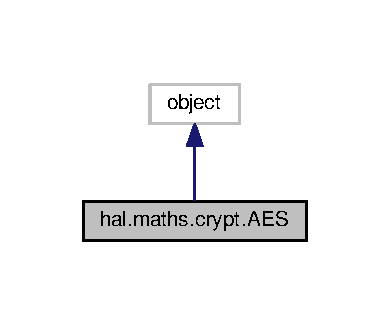
\includegraphics[width=187pt]{classhal_1_1maths_1_1crypt_1_1_a_e_s__inherit__graph}
\end{center}
\end{figure}


Collaboration diagram for hal.\+maths.\+crypt.\+A\+ES\+:
\nopagebreak
\begin{figure}[H]
\begin{center}
\leavevmode
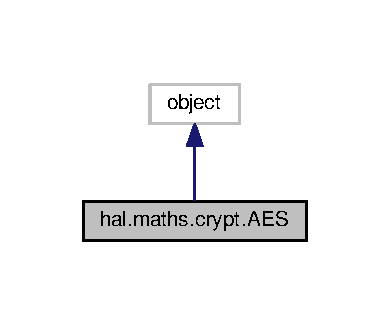
\includegraphics[width=187pt]{classhal_1_1maths_1_1crypt_1_1_a_e_s__coll__graph}
\end{center}
\end{figure}
\subsection*{Public Member Functions}
\begin{DoxyCompactItemize}
\item 
def {\bfseries \+\_\+\+\_\+init\+\_\+\+\_\+} (self, string, key)\hypertarget{classhal_1_1maths_1_1crypt_1_1_a_e_s_a384607218f6de8a5bf2091a8913f02a2}{}\label{classhal_1_1maths_1_1crypt_1_1_a_e_s_a384607218f6de8a5bf2091a8913f02a2}

\item 
def \hyperlink{classhal_1_1maths_1_1crypt_1_1_a_e_s_ab7bd23c02bda2da94f6a2437f906cd09}{hash} (self)
\end{DoxyCompactItemize}
\subsection*{Public Attributes}
\begin{DoxyCompactItemize}
\item 
{\bfseries plain}\hypertarget{classhal_1_1maths_1_1crypt_1_1_a_e_s_a511e51110acb8e0ff377a021458d89ec}{}\label{classhal_1_1maths_1_1crypt_1_1_a_e_s_a511e51110acb8e0ff377a021458d89ec}

\item 
{\bfseries key}\hypertarget{classhal_1_1maths_1_1crypt_1_1_a_e_s_a41c89cf1e5822b1b1831132c2cb50c8c}{}\label{classhal_1_1maths_1_1crypt_1_1_a_e_s_a41c89cf1e5822b1b1831132c2cb50c8c}

\item 
{\bfseries hashed}\hypertarget{classhal_1_1maths_1_1crypt_1_1_a_e_s_a7a203fbe4d7cd5ce3c170c8d163d9587}{}\label{classhal_1_1maths_1_1crypt_1_1_a_e_s_a7a203fbe4d7cd5ce3c170c8d163d9587}

\end{DoxyCompactItemize}


\subsection{Detailed Description}
\begin{DoxyVerb}aes hash \end{DoxyVerb}
 

\subsection{Member Function Documentation}
\index{hal\+::maths\+::crypt\+::\+A\+ES@{hal\+::maths\+::crypt\+::\+A\+ES}!hash@{hash}}
\index{hash@{hash}!hal\+::maths\+::crypt\+::\+A\+ES@{hal\+::maths\+::crypt\+::\+A\+ES}}
\subsubsection[{\texorpdfstring{hash(self)}{hash(self)}}]{\setlength{\rightskip}{0pt plus 5cm}def hal.\+maths.\+crypt.\+A\+E\+S.\+hash (
\begin{DoxyParamCaption}
\item[{}]{self}
\end{DoxyParamCaption}
)}\hypertarget{classhal_1_1maths_1_1crypt_1_1_a_e_s_ab7bd23c02bda2da94f6a2437f906cd09}{}\label{classhal_1_1maths_1_1crypt_1_1_a_e_s_ab7bd23c02bda2da94f6a2437f906cd09}
\begin{DoxyVerb}:return: hash plaintext
\end{DoxyVerb}
 

The documentation for this class was generated from the following file\+:\begin{DoxyCompactItemize}
\item 
hal/maths/crypt.\+py\end{DoxyCompactItemize}

\hypertarget{classhal_1_1maths_1_1crypt_1_1_a_r_c}{}\section{hal.\+maths.\+crypt.\+A\+RC Class Reference}
\label{classhal_1_1maths_1_1crypt_1_1_a_r_c}\index{hal.\+maths.\+crypt.\+A\+RC@{hal.\+maths.\+crypt.\+A\+RC}}


Inheritance diagram for hal.\+maths.\+crypt.\+A\+RC\+:
\nopagebreak
\begin{figure}[H]
\begin{center}
\leavevmode
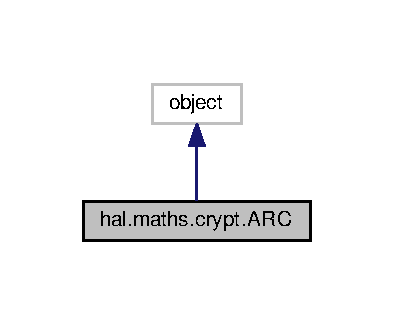
\includegraphics[width=189pt]{classhal_1_1maths_1_1crypt_1_1_a_r_c__inherit__graph}
\end{center}
\end{figure}


Collaboration diagram for hal.\+maths.\+crypt.\+A\+RC\+:
\nopagebreak
\begin{figure}[H]
\begin{center}
\leavevmode
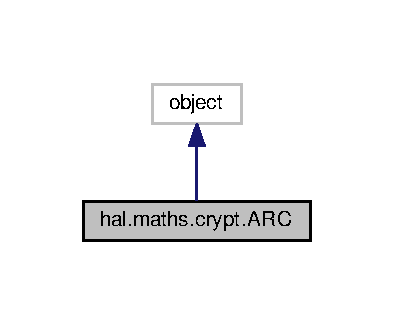
\includegraphics[width=189pt]{classhal_1_1maths_1_1crypt_1_1_a_r_c__coll__graph}
\end{center}
\end{figure}
\subsection*{Public Member Functions}
\begin{DoxyCompactItemize}
\item 
def {\bfseries \+\_\+\+\_\+init\+\_\+\+\_\+} (self, string, key, size)\hypertarget{classhal_1_1maths_1_1crypt_1_1_a_r_c_a82309db9054f68f3f2c9b5eea7e46c3d}{}\label{classhal_1_1maths_1_1crypt_1_1_a_r_c_a82309db9054f68f3f2c9b5eea7e46c3d}

\item 
def \hyperlink{classhal_1_1maths_1_1crypt_1_1_a_r_c_a5453d043fc6d569e8d56b08d0657440d}{hash} (self)
\item 
def \hyperlink{classhal_1_1maths_1_1crypt_1_1_a_r_c_a8bb650cb7e154c93c8d3f90939e42330}{hash\+\_\+ar2} (self)
\item 
def \hyperlink{classhal_1_1maths_1_1crypt_1_1_a_r_c_ad81bf4a4f683f4c303c05c6ae93fb020}{hash\+\_\+arc4} (self)
\end{DoxyCompactItemize}
\subsection*{Public Attributes}
\begin{DoxyCompactItemize}
\item 
{\bfseries plain}\hypertarget{classhal_1_1maths_1_1crypt_1_1_a_r_c_ab565094fdb53f56635001d60863153c7}{}\label{classhal_1_1maths_1_1crypt_1_1_a_r_c_ab565094fdb53f56635001d60863153c7}

\item 
{\bfseries key}\hypertarget{classhal_1_1maths_1_1crypt_1_1_a_r_c_a21a38c518574b0558238889bc0632e24}{}\label{classhal_1_1maths_1_1crypt_1_1_a_r_c_a21a38c518574b0558238889bc0632e24}

\item 
{\bfseries size}\hypertarget{classhal_1_1maths_1_1crypt_1_1_a_r_c_a87c67dc38f9fd683d3f16f5b27a125a3}{}\label{classhal_1_1maths_1_1crypt_1_1_a_r_c_a87c67dc38f9fd683d3f16f5b27a125a3}

\item 
{\bfseries hashed}\hypertarget{classhal_1_1maths_1_1crypt_1_1_a_r_c_ad6d70770753dd95fd685f11aa2c50f35}{}\label{classhal_1_1maths_1_1crypt_1_1_a_r_c_ad6d70770753dd95fd685f11aa2c50f35}

\end{DoxyCompactItemize}
\subsection*{Static Public Attributes}
\begin{DoxyCompactItemize}
\item 
list {\bfseries A\+L\+L\+O\+W\+E\+D\+\_\+\+S\+I\+ZE} = \mbox{[}2, 4\mbox{]}\hypertarget{classhal_1_1maths_1_1crypt_1_1_a_r_c_add5e33fd8bbab7761bc77f633363c5a0}{}\label{classhal_1_1maths_1_1crypt_1_1_a_r_c_add5e33fd8bbab7761bc77f633363c5a0}

\end{DoxyCompactItemize}


\subsection{Detailed Description}
\begin{DoxyVerb}ARC hash \end{DoxyVerb}
 

\subsection{Member Function Documentation}
\index{hal\+::maths\+::crypt\+::\+A\+RC@{hal\+::maths\+::crypt\+::\+A\+RC}!hash@{hash}}
\index{hash@{hash}!hal\+::maths\+::crypt\+::\+A\+RC@{hal\+::maths\+::crypt\+::\+A\+RC}}
\subsubsection[{\texorpdfstring{hash(self)}{hash(self)}}]{\setlength{\rightskip}{0pt plus 5cm}def hal.\+maths.\+crypt.\+A\+R\+C.\+hash (
\begin{DoxyParamCaption}
\item[{}]{self}
\end{DoxyParamCaption}
)}\hypertarget{classhal_1_1maths_1_1crypt_1_1_a_r_c_a5453d043fc6d569e8d56b08d0657440d}{}\label{classhal_1_1maths_1_1crypt_1_1_a_r_c_a5453d043fc6d569e8d56b08d0657440d}
\begin{DoxyVerb}:return: hash of given size
\end{DoxyVerb}
 \index{hal\+::maths\+::crypt\+::\+A\+RC@{hal\+::maths\+::crypt\+::\+A\+RC}!hash\+\_\+ar2@{hash\+\_\+ar2}}
\index{hash\+\_\+ar2@{hash\+\_\+ar2}!hal\+::maths\+::crypt\+::\+A\+RC@{hal\+::maths\+::crypt\+::\+A\+RC}}
\subsubsection[{\texorpdfstring{hash\+\_\+ar2(self)}{hash_ar2(self)}}]{\setlength{\rightskip}{0pt plus 5cm}def hal.\+maths.\+crypt.\+A\+R\+C.\+hash\+\_\+ar2 (
\begin{DoxyParamCaption}
\item[{}]{self}
\end{DoxyParamCaption}
)}\hypertarget{classhal_1_1maths_1_1crypt_1_1_a_r_c_a8bb650cb7e154c93c8d3f90939e42330}{}\label{classhal_1_1maths_1_1crypt_1_1_a_r_c_a8bb650cb7e154c93c8d3f90939e42330}
\begin{DoxyVerb}:return: des hash
\end{DoxyVerb}
 \index{hal\+::maths\+::crypt\+::\+A\+RC@{hal\+::maths\+::crypt\+::\+A\+RC}!hash\+\_\+arc4@{hash\+\_\+arc4}}
\index{hash\+\_\+arc4@{hash\+\_\+arc4}!hal\+::maths\+::crypt\+::\+A\+RC@{hal\+::maths\+::crypt\+::\+A\+RC}}
\subsubsection[{\texorpdfstring{hash\+\_\+arc4(self)}{hash_arc4(self)}}]{\setlength{\rightskip}{0pt plus 5cm}def hal.\+maths.\+crypt.\+A\+R\+C.\+hash\+\_\+arc4 (
\begin{DoxyParamCaption}
\item[{}]{self}
\end{DoxyParamCaption}
)}\hypertarget{classhal_1_1maths_1_1crypt_1_1_a_r_c_ad81bf4a4f683f4c303c05c6ae93fb020}{}\label{classhal_1_1maths_1_1crypt_1_1_a_r_c_ad81bf4a4f683f4c303c05c6ae93fb020}
\begin{DoxyVerb}:return: des3 hash
\end{DoxyVerb}
 

The documentation for this class was generated from the following file\+:\begin{DoxyCompactItemize}
\item 
hal/maths/crypt.\+py\end{DoxyCompactItemize}

\hypertarget{classhal_1_1ml_1_1predict_1_1_base_prediction}{}\section{hal.\+ml.\+predict.\+Base\+Prediction Class Reference}
\label{classhal_1_1ml_1_1predict_1_1_base_prediction}\index{hal.\+ml.\+predict.\+Base\+Prediction@{hal.\+ml.\+predict.\+Base\+Prediction}}


Inheritance diagram for hal.\+ml.\+predict.\+Base\+Prediction\+:\nopagebreak
\begin{figure}[H]
\begin{center}
\leavevmode
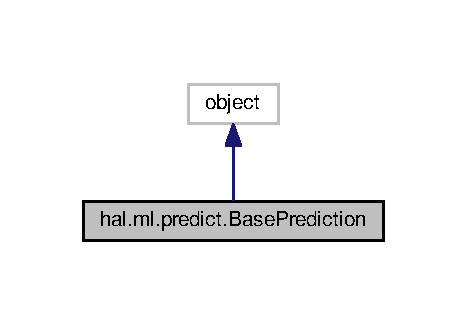
\includegraphics[width=224pt]{classhal_1_1ml_1_1predict_1_1_base_prediction__inherit__graph}
\end{center}
\end{figure}


Collaboration diagram for hal.\+ml.\+predict.\+Base\+Prediction\+:\nopagebreak
\begin{figure}[H]
\begin{center}
\leavevmode
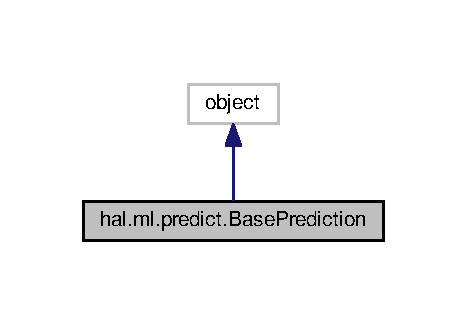
\includegraphics[width=224pt]{classhal_1_1ml_1_1predict_1_1_base_prediction__coll__graph}
\end{center}
\end{figure}
\subsection*{Public Member Functions}
\begin{DoxyCompactItemize}
\item 
def {\bfseries \+\_\+\+\_\+init\+\_\+\+\_\+} (self, model, rounds)\hypertarget{classhal_1_1ml_1_1predict_1_1_base_prediction_a77743bfb5de4846d30d3f41e7d2706df}{}\label{classhal_1_1ml_1_1predict_1_1_base_prediction_a77743bfb5de4846d30d3f41e7d2706df}

\item 
def {\bfseries train} (self, x, y)\hypertarget{classhal_1_1ml_1_1predict_1_1_base_prediction_a3bee607838f71f2ed205864a3f73d5f5}{}\label{classhal_1_1ml_1_1predict_1_1_base_prediction_a3bee607838f71f2ed205864a3f73d5f5}

\end{DoxyCompactItemize}
\subsection*{Public Attributes}
\begin{DoxyCompactItemize}
\item 
{\bfseries model}\hypertarget{classhal_1_1ml_1_1predict_1_1_base_prediction_a78a5950426761d76607463957e6d7b5f}{}\label{classhal_1_1ml_1_1predict_1_1_base_prediction_a78a5950426761d76607463957e6d7b5f}

\item 
{\bfseries rounds}\hypertarget{classhal_1_1ml_1_1predict_1_1_base_prediction_a706bdbfbad676c63b8755e43189d706f}{}\label{classhal_1_1ml_1_1predict_1_1_base_prediction_a706bdbfbad676c63b8755e43189d706f}

\end{DoxyCompactItemize}


The documentation for this class was generated from the following file\+:\begin{DoxyCompactItemize}
\item 
/home/stefano/\+Coding/\+Python/projects/pyhal/hal/ml/predict.\+py\end{DoxyCompactItemize}

\hypertarget{classhal_1_1maths_1_1crypt_1_1_b_l_o_w_f_i_s_h}{}\section{hal.\+maths.\+crypt.\+B\+L\+O\+W\+F\+I\+SH Class Reference}
\label{classhal_1_1maths_1_1crypt_1_1_b_l_o_w_f_i_s_h}\index{hal.\+maths.\+crypt.\+B\+L\+O\+W\+F\+I\+SH@{hal.\+maths.\+crypt.\+B\+L\+O\+W\+F\+I\+SH}}


Inheritance diagram for hal.\+maths.\+crypt.\+B\+L\+O\+W\+F\+I\+SH\+:\nopagebreak
\begin{figure}[H]
\begin{center}
\leavevmode
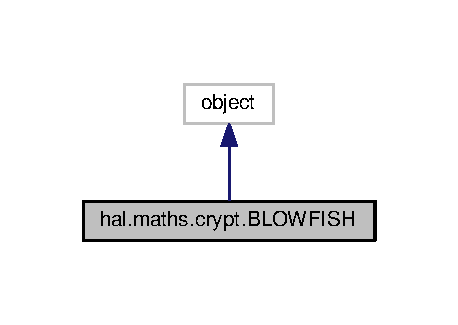
\includegraphics[width=220pt]{classhal_1_1maths_1_1crypt_1_1_b_l_o_w_f_i_s_h__inherit__graph}
\end{center}
\end{figure}


Collaboration diagram for hal.\+maths.\+crypt.\+B\+L\+O\+W\+F\+I\+SH\+:\nopagebreak
\begin{figure}[H]
\begin{center}
\leavevmode
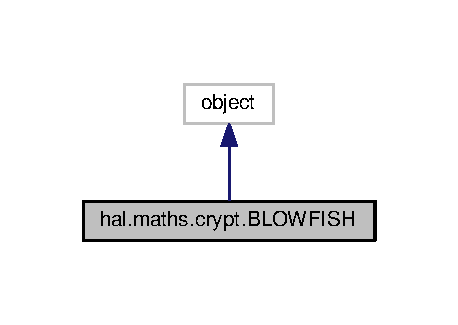
\includegraphics[width=220pt]{classhal_1_1maths_1_1crypt_1_1_b_l_o_w_f_i_s_h__coll__graph}
\end{center}
\end{figure}
\subsection*{Public Member Functions}
\begin{DoxyCompactItemize}
\item 
def {\bfseries \+\_\+\+\_\+init\+\_\+\+\_\+} (self, string, key)\hypertarget{classhal_1_1maths_1_1crypt_1_1_b_l_o_w_f_i_s_h_a0428f1f9b864c84c1911d61235e739fc}{}\label{classhal_1_1maths_1_1crypt_1_1_b_l_o_w_f_i_s_h_a0428f1f9b864c84c1911d61235e739fc}

\item 
def \hyperlink{classhal_1_1maths_1_1crypt_1_1_b_l_o_w_f_i_s_h_a7581e9c15acfe4cb64c88c215193f65a}{hash} (self)
\end{DoxyCompactItemize}
\subsection*{Public Attributes}
\begin{DoxyCompactItemize}
\item 
{\bfseries plain}\hypertarget{classhal_1_1maths_1_1crypt_1_1_b_l_o_w_f_i_s_h_a91433d504d000422abfce6ad4df9fed5}{}\label{classhal_1_1maths_1_1crypt_1_1_b_l_o_w_f_i_s_h_a91433d504d000422abfce6ad4df9fed5}

\item 
{\bfseries key}\hypertarget{classhal_1_1maths_1_1crypt_1_1_b_l_o_w_f_i_s_h_a6c4537a3fff285916787aea66f8286b6}{}\label{classhal_1_1maths_1_1crypt_1_1_b_l_o_w_f_i_s_h_a6c4537a3fff285916787aea66f8286b6}

\item 
{\bfseries hashed}\hypertarget{classhal_1_1maths_1_1crypt_1_1_b_l_o_w_f_i_s_h_a315f4ff71730a1c60b97324e41475e48}{}\label{classhal_1_1maths_1_1crypt_1_1_b_l_o_w_f_i_s_h_a315f4ff71730a1c60b97324e41475e48}

\end{DoxyCompactItemize}


\subsection{Detailed Description}
\begin{DoxyVerb}blowfish hash \end{DoxyVerb}
 

\subsection{Member Function Documentation}
\index{hal\+::maths\+::crypt\+::\+B\+L\+O\+W\+F\+I\+SH@{hal\+::maths\+::crypt\+::\+B\+L\+O\+W\+F\+I\+SH}!hash@{hash}}
\index{hash@{hash}!hal\+::maths\+::crypt\+::\+B\+L\+O\+W\+F\+I\+SH@{hal\+::maths\+::crypt\+::\+B\+L\+O\+W\+F\+I\+SH}}
\subsubsection[{\texorpdfstring{hash(self)}{hash(self)}}]{\setlength{\rightskip}{0pt plus 5cm}def hal.\+maths.\+crypt.\+B\+L\+O\+W\+F\+I\+S\+H.\+hash (
\begin{DoxyParamCaption}
\item[{}]{self}
\end{DoxyParamCaption}
)}\hypertarget{classhal_1_1maths_1_1crypt_1_1_b_l_o_w_f_i_s_h_a7581e9c15acfe4cb64c88c215193f65a}{}\label{classhal_1_1maths_1_1crypt_1_1_b_l_o_w_f_i_s_h_a7581e9c15acfe4cb64c88c215193f65a}
\begin{DoxyVerb}:return: hash plaintext
\end{DoxyVerb}
 

The documentation for this class was generated from the following file\+:\begin{DoxyCompactItemize}
\item 
/home/stefano/\+Coding/\+Python/projects/pyhal/hal/maths/crypt.\+py\end{DoxyCompactItemize}

\hypertarget{classhal_1_1maths_1_1crypt_1_1_c_a_s_t128}{}\section{hal.\+maths.\+crypt.\+C\+A\+S\+T128 Class Reference}
\label{classhal_1_1maths_1_1crypt_1_1_c_a_s_t128}\index{hal.\+maths.\+crypt.\+C\+A\+S\+T128@{hal.\+maths.\+crypt.\+C\+A\+S\+T128}}


Inheritance diagram for hal.\+maths.\+crypt.\+C\+A\+S\+T128\+:\nopagebreak
\begin{figure}[H]
\begin{center}
\leavevmode
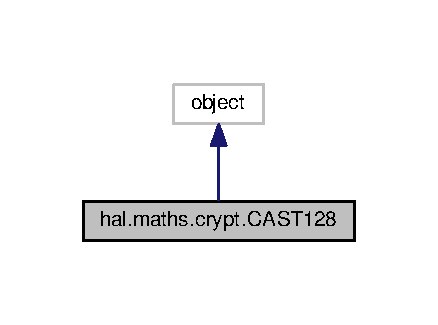
\includegraphics[width=210pt]{classhal_1_1maths_1_1crypt_1_1_c_a_s_t128__inherit__graph}
\end{center}
\end{figure}


Collaboration diagram for hal.\+maths.\+crypt.\+C\+A\+S\+T128\+:\nopagebreak
\begin{figure}[H]
\begin{center}
\leavevmode
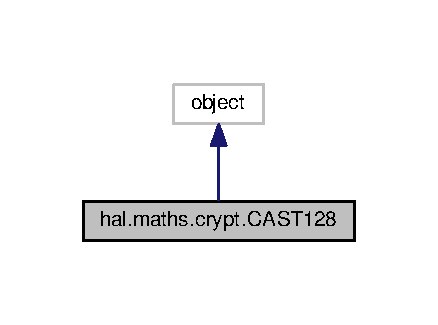
\includegraphics[width=210pt]{classhal_1_1maths_1_1crypt_1_1_c_a_s_t128__coll__graph}
\end{center}
\end{figure}
\subsection*{Public Member Functions}
\begin{DoxyCompactItemize}
\item 
def {\bfseries \+\_\+\+\_\+init\+\_\+\+\_\+} (self, string, key)\hypertarget{classhal_1_1maths_1_1crypt_1_1_c_a_s_t128_a285a3b0d8e5ab5a6aa1bfe2ed07cf275}{}\label{classhal_1_1maths_1_1crypt_1_1_c_a_s_t128_a285a3b0d8e5ab5a6aa1bfe2ed07cf275}

\item 
def \hyperlink{classhal_1_1maths_1_1crypt_1_1_c_a_s_t128_a955fa0eab07e305ba028b007c2851abf}{encrypt} (self)
\item 
def \hyperlink{classhal_1_1maths_1_1crypt_1_1_c_a_s_t128_a70b29321e653c2daaeb2c9e144d2c1c0}{decrypt} (self)
\end{DoxyCompactItemize}
\subsection*{Public Attributes}
\begin{DoxyCompactItemize}
\item 
{\bfseries plain}\hypertarget{classhal_1_1maths_1_1crypt_1_1_c_a_s_t128_af91078dab517ef6705a17f5c41821d27}{}\label{classhal_1_1maths_1_1crypt_1_1_c_a_s_t128_af91078dab517ef6705a17f5c41821d27}

\item 
{\bfseries key}\hypertarget{classhal_1_1maths_1_1crypt_1_1_c_a_s_t128_af89de906c01f3aa02c872831548307a6}{}\label{classhal_1_1maths_1_1crypt_1_1_c_a_s_t128_af89de906c01f3aa02c872831548307a6}

\item 
{\bfseries answer}\hypertarget{classhal_1_1maths_1_1crypt_1_1_c_a_s_t128_a452da0fec6f88f16ec468ceaa55b3d18}{}\label{classhal_1_1maths_1_1crypt_1_1_c_a_s_t128_a452da0fec6f88f16ec468ceaa55b3d18}

\end{DoxyCompactItemize}


\subsection{Detailed Description}
\begin{DoxyVerb}CAST 128 hash \end{DoxyVerb}
 

\subsection{Member Function Documentation}
\index{hal\+::maths\+::crypt\+::\+C\+A\+S\+T128@{hal\+::maths\+::crypt\+::\+C\+A\+S\+T128}!decrypt@{decrypt}}
\index{decrypt@{decrypt}!hal\+::maths\+::crypt\+::\+C\+A\+S\+T128@{hal\+::maths\+::crypt\+::\+C\+A\+S\+T128}}
\subsubsection[{\texorpdfstring{decrypt(self)}{decrypt(self)}}]{\setlength{\rightskip}{0pt plus 5cm}def hal.\+maths.\+crypt.\+C\+A\+S\+T128.\+decrypt (
\begin{DoxyParamCaption}
\item[{}]{self}
\end{DoxyParamCaption}
)}\hypertarget{classhal_1_1maths_1_1crypt_1_1_c_a_s_t128_a70b29321e653c2daaeb2c9e144d2c1c0}{}\label{classhal_1_1maths_1_1crypt_1_1_c_a_s_t128_a70b29321e653c2daaeb2c9e144d2c1c0}
\begin{DoxyVerb}:return: str
    Decrypt
\end{DoxyVerb}
 \index{hal\+::maths\+::crypt\+::\+C\+A\+S\+T128@{hal\+::maths\+::crypt\+::\+C\+A\+S\+T128}!encrypt@{encrypt}}
\index{encrypt@{encrypt}!hal\+::maths\+::crypt\+::\+C\+A\+S\+T128@{hal\+::maths\+::crypt\+::\+C\+A\+S\+T128}}
\subsubsection[{\texorpdfstring{encrypt(self)}{encrypt(self)}}]{\setlength{\rightskip}{0pt plus 5cm}def hal.\+maths.\+crypt.\+C\+A\+S\+T128.\+encrypt (
\begin{DoxyParamCaption}
\item[{}]{self}
\end{DoxyParamCaption}
)}\hypertarget{classhal_1_1maths_1_1crypt_1_1_c_a_s_t128_a955fa0eab07e305ba028b007c2851abf}{}\label{classhal_1_1maths_1_1crypt_1_1_c_a_s_t128_a955fa0eab07e305ba028b007c2851abf}
\begin{DoxyVerb}:return: str
    Encrypt
\end{DoxyVerb}
 

The documentation for this class was generated from the following file\+:\begin{DoxyCompactItemize}
\item 
/home/stefano/\+Coding/\+Python/projects/pyhal/hal/maths/crypt.\+py\end{DoxyCompactItemize}

\hypertarget{classhal_1_1ml_1_1data_1_1parser_1_1_c_s_v_parser}{}\section{hal.\+ml.\+data.\+parser.\+C\+S\+V\+Parser Class Reference}
\label{classhal_1_1ml_1_1data_1_1parser_1_1_c_s_v_parser}\index{hal.\+ml.\+data.\+parser.\+C\+S\+V\+Parser@{hal.\+ml.\+data.\+parser.\+C\+S\+V\+Parser}}


Inheritance diagram for hal.\+ml.\+data.\+parser.\+C\+S\+V\+Parser\+:
\nopagebreak
\begin{figure}[H]
\begin{center}
\leavevmode
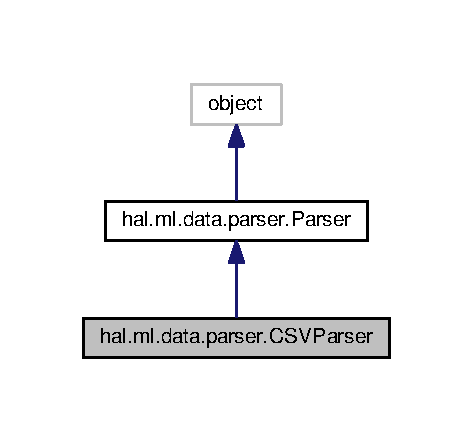
\includegraphics[width=227pt]{classhal_1_1ml_1_1data_1_1parser_1_1_c_s_v_parser__inherit__graph}
\end{center}
\end{figure}


Collaboration diagram for hal.\+ml.\+data.\+parser.\+C\+S\+V\+Parser\+:
\nopagebreak
\begin{figure}[H]
\begin{center}
\leavevmode
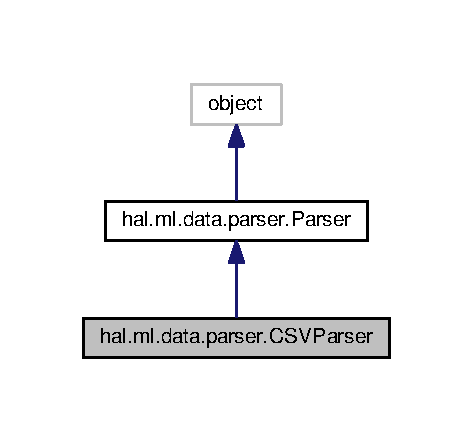
\includegraphics[width=227pt]{classhal_1_1ml_1_1data_1_1parser_1_1_c_s_v_parser__coll__graph}
\end{center}
\end{figure}
\subsection*{Public Member Functions}
\begin{DoxyCompactItemize}
\item 
def \hyperlink{classhal_1_1ml_1_1data_1_1parser_1_1_c_s_v_parser_adb6168a2083f75a99132b4aad471b9e6}{\+\_\+\+\_\+init\+\_\+\+\_\+} (self, database\+\_\+file)
\item 
def \hyperlink{classhal_1_1ml_1_1data_1_1parser_1_1_c_s_v_parser_ac47a4070d172a1ada61060610749f5e8}{parse\+\_\+data} (self)
\end{DoxyCompactItemize}
\subsection*{Public Attributes}
\begin{DoxyCompactItemize}
\item 
{\bfseries data}\hypertarget{classhal_1_1ml_1_1data_1_1parser_1_1_c_s_v_parser_a1119c3b0d27312ff8086f710a71a8bf2}{}\label{classhal_1_1ml_1_1data_1_1parser_1_1_c_s_v_parser_a1119c3b0d27312ff8086f710a71a8bf2}

\end{DoxyCompactItemize}


\subsection{Constructor \& Destructor Documentation}
\index{hal\+::ml\+::data\+::parser\+::\+C\+S\+V\+Parser@{hal\+::ml\+::data\+::parser\+::\+C\+S\+V\+Parser}!\+\_\+\+\_\+init\+\_\+\+\_\+@{\+\_\+\+\_\+init\+\_\+\+\_\+}}
\index{\+\_\+\+\_\+init\+\_\+\+\_\+@{\+\_\+\+\_\+init\+\_\+\+\_\+}!hal\+::ml\+::data\+::parser\+::\+C\+S\+V\+Parser@{hal\+::ml\+::data\+::parser\+::\+C\+S\+V\+Parser}}
\subsubsection[{\texorpdfstring{\+\_\+\+\_\+init\+\_\+\+\_\+(self, database\+\_\+file)}{__init__(self, database_file)}}]{\setlength{\rightskip}{0pt plus 5cm}def hal.\+ml.\+data.\+parser.\+C\+S\+V\+Parser.\+\_\+\+\_\+init\+\_\+\+\_\+ (
\begin{DoxyParamCaption}
\item[{}]{self, }
\item[{}]{database\+\_\+file}
\end{DoxyParamCaption}
)}\hypertarget{classhal_1_1ml_1_1data_1_1parser_1_1_c_s_v_parser_adb6168a2083f75a99132b4aad471b9e6}{}\label{classhal_1_1ml_1_1data_1_1parser_1_1_c_s_v_parser_adb6168a2083f75a99132b4aad471b9e6}
\begin{DoxyVerb}:param database_file: a raw .csv file that contains any data about anything \end{DoxyVerb}
 

\subsection{Member Function Documentation}
\index{hal\+::ml\+::data\+::parser\+::\+C\+S\+V\+Parser@{hal\+::ml\+::data\+::parser\+::\+C\+S\+V\+Parser}!parse\+\_\+data@{parse\+\_\+data}}
\index{parse\+\_\+data@{parse\+\_\+data}!hal\+::ml\+::data\+::parser\+::\+C\+S\+V\+Parser@{hal\+::ml\+::data\+::parser\+::\+C\+S\+V\+Parser}}
\subsubsection[{\texorpdfstring{parse\+\_\+data(self)}{parse_data(self)}}]{\setlength{\rightskip}{0pt plus 5cm}def hal.\+ml.\+data.\+parser.\+C\+S\+V\+Parser.\+parse\+\_\+data (
\begin{DoxyParamCaption}
\item[{}]{self}
\end{DoxyParamCaption}
)}\hypertarget{classhal_1_1ml_1_1data_1_1parser_1_1_c_s_v_parser_ac47a4070d172a1ada61060610749f5e8}{}\label{classhal_1_1ml_1_1data_1_1parser_1_1_c_s_v_parser_ac47a4070d172a1ada61060610749f5e8}
\begin{DoxyVerb}store values in array, store lines in array; the result is a 2D matrix\end{DoxyVerb}
 

The documentation for this class was generated from the following file\+:\begin{DoxyCompactItemize}
\item 
hal/ml/data/parser.\+py\end{DoxyCompactItemize}

\hypertarget{classhal_1_1maths_1_1crypt_1_1_d_e_s}{}\section{hal.\+maths.\+crypt.\+D\+ES Class Reference}
\label{classhal_1_1maths_1_1crypt_1_1_d_e_s}\index{hal.\+maths.\+crypt.\+D\+ES@{hal.\+maths.\+crypt.\+D\+ES}}


Inheritance diagram for hal.\+maths.\+crypt.\+D\+ES\+:
\nopagebreak
\begin{figure}[H]
\begin{center}
\leavevmode
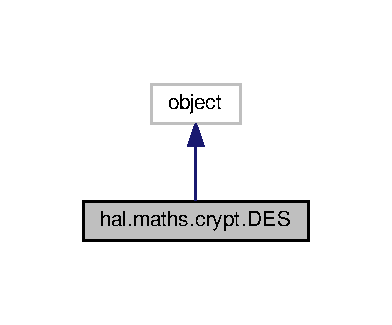
\includegraphics[width=188pt]{classhal_1_1maths_1_1crypt_1_1_d_e_s__inherit__graph}
\end{center}
\end{figure}


Collaboration diagram for hal.\+maths.\+crypt.\+D\+ES\+:
\nopagebreak
\begin{figure}[H]
\begin{center}
\leavevmode
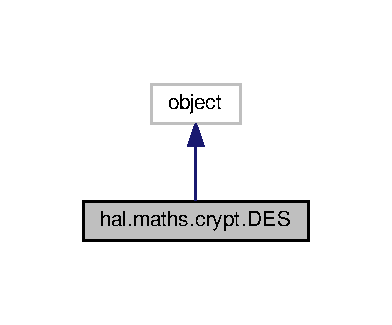
\includegraphics[width=188pt]{classhal_1_1maths_1_1crypt_1_1_d_e_s__coll__graph}
\end{center}
\end{figure}
\subsection*{Public Member Functions}
\begin{DoxyCompactItemize}
\item 
def {\bfseries \+\_\+\+\_\+init\+\_\+\+\_\+} (self, string, key, size)\hypertarget{classhal_1_1maths_1_1crypt_1_1_d_e_s_a163fe40de3514de90bf07230f18cb891}{}\label{classhal_1_1maths_1_1crypt_1_1_d_e_s_a163fe40de3514de90bf07230f18cb891}

\item 
def \hyperlink{classhal_1_1maths_1_1crypt_1_1_d_e_s_a950a921233fa101b5be1c2910c1e0595}{hash} (self)
\item 
def \hyperlink{classhal_1_1maths_1_1crypt_1_1_d_e_s_a0e397526a54b62510f118a0859b3c8b6}{hash\+\_\+des} (self)
\item 
def \hyperlink{classhal_1_1maths_1_1crypt_1_1_d_e_s_a9183df60a448c690beb8ac117262aa41}{hash\+\_\+des3} (self)
\end{DoxyCompactItemize}
\subsection*{Public Attributes}
\begin{DoxyCompactItemize}
\item 
{\bfseries plain}\hypertarget{classhal_1_1maths_1_1crypt_1_1_d_e_s_a7f7043d08dd641c3e061d6316263754a}{}\label{classhal_1_1maths_1_1crypt_1_1_d_e_s_a7f7043d08dd641c3e061d6316263754a}

\item 
{\bfseries key}\hypertarget{classhal_1_1maths_1_1crypt_1_1_d_e_s_a5220f18392796674edee54db1772365b}{}\label{classhal_1_1maths_1_1crypt_1_1_d_e_s_a5220f18392796674edee54db1772365b}

\item 
{\bfseries size}\hypertarget{classhal_1_1maths_1_1crypt_1_1_d_e_s_a0197f3353d660bba2ee2046b0e27ff4f}{}\label{classhal_1_1maths_1_1crypt_1_1_d_e_s_a0197f3353d660bba2ee2046b0e27ff4f}

\item 
{\bfseries hashed}\hypertarget{classhal_1_1maths_1_1crypt_1_1_d_e_s_a413aae8583c759879becd80f35dd335d}{}\label{classhal_1_1maths_1_1crypt_1_1_d_e_s_a413aae8583c759879becd80f35dd335d}

\end{DoxyCompactItemize}
\subsection*{Static Public Attributes}
\begin{DoxyCompactItemize}
\item 
list {\bfseries A\+L\+L\+O\+W\+E\+D\+\_\+\+S\+I\+ZE} = \mbox{[}1, 3\mbox{]}\hypertarget{classhal_1_1maths_1_1crypt_1_1_d_e_s_af4a6996632dc4bc9711ec4f17ca3c425}{}\label{classhal_1_1maths_1_1crypt_1_1_d_e_s_af4a6996632dc4bc9711ec4f17ca3c425}

\end{DoxyCompactItemize}


\subsection{Detailed Description}
\begin{DoxyVerb}DES hash \end{DoxyVerb}
 

\subsection{Member Function Documentation}
\index{hal\+::maths\+::crypt\+::\+D\+ES@{hal\+::maths\+::crypt\+::\+D\+ES}!hash@{hash}}
\index{hash@{hash}!hal\+::maths\+::crypt\+::\+D\+ES@{hal\+::maths\+::crypt\+::\+D\+ES}}
\subsubsection[{\texorpdfstring{hash(self)}{hash(self)}}]{\setlength{\rightskip}{0pt plus 5cm}def hal.\+maths.\+crypt.\+D\+E\+S.\+hash (
\begin{DoxyParamCaption}
\item[{}]{self}
\end{DoxyParamCaption}
)}\hypertarget{classhal_1_1maths_1_1crypt_1_1_d_e_s_a950a921233fa101b5be1c2910c1e0595}{}\label{classhal_1_1maths_1_1crypt_1_1_d_e_s_a950a921233fa101b5be1c2910c1e0595}
\begin{DoxyVerb}:return: hash of given size
\end{DoxyVerb}
 \index{hal\+::maths\+::crypt\+::\+D\+ES@{hal\+::maths\+::crypt\+::\+D\+ES}!hash\+\_\+des@{hash\+\_\+des}}
\index{hash\+\_\+des@{hash\+\_\+des}!hal\+::maths\+::crypt\+::\+D\+ES@{hal\+::maths\+::crypt\+::\+D\+ES}}
\subsubsection[{\texorpdfstring{hash\+\_\+des(self)}{hash_des(self)}}]{\setlength{\rightskip}{0pt plus 5cm}def hal.\+maths.\+crypt.\+D\+E\+S.\+hash\+\_\+des (
\begin{DoxyParamCaption}
\item[{}]{self}
\end{DoxyParamCaption}
)}\hypertarget{classhal_1_1maths_1_1crypt_1_1_d_e_s_a0e397526a54b62510f118a0859b3c8b6}{}\label{classhal_1_1maths_1_1crypt_1_1_d_e_s_a0e397526a54b62510f118a0859b3c8b6}
\begin{DoxyVerb}:return: des hash
\end{DoxyVerb}
 \index{hal\+::maths\+::crypt\+::\+D\+ES@{hal\+::maths\+::crypt\+::\+D\+ES}!hash\+\_\+des3@{hash\+\_\+des3}}
\index{hash\+\_\+des3@{hash\+\_\+des3}!hal\+::maths\+::crypt\+::\+D\+ES@{hal\+::maths\+::crypt\+::\+D\+ES}}
\subsubsection[{\texorpdfstring{hash\+\_\+des3(self)}{hash_des3(self)}}]{\setlength{\rightskip}{0pt plus 5cm}def hal.\+maths.\+crypt.\+D\+E\+S.\+hash\+\_\+des3 (
\begin{DoxyParamCaption}
\item[{}]{self}
\end{DoxyParamCaption}
)}\hypertarget{classhal_1_1maths_1_1crypt_1_1_d_e_s_a9183df60a448c690beb8ac117262aa41}{}\label{classhal_1_1maths_1_1crypt_1_1_d_e_s_a9183df60a448c690beb8ac117262aa41}
\begin{DoxyVerb}:return: des3 hash
\end{DoxyVerb}
 

The documentation for this class was generated from the following file\+:\begin{DoxyCompactItemize}
\item 
hal/maths/crypt.\+py\end{DoxyCompactItemize}

\hypertarget{classhal_1_1files_1_1models_1_1_directory}{}\section{hal.\+files.\+models.\+Directory Class Reference}
\label{classhal_1_1files_1_1models_1_1_directory}\index{hal.\+files.\+models.\+Directory@{hal.\+files.\+models.\+Directory}}


Inheritance diagram for hal.\+files.\+models.\+Directory\+:
\nopagebreak
\begin{figure}[H]
\begin{center}
\leavevmode
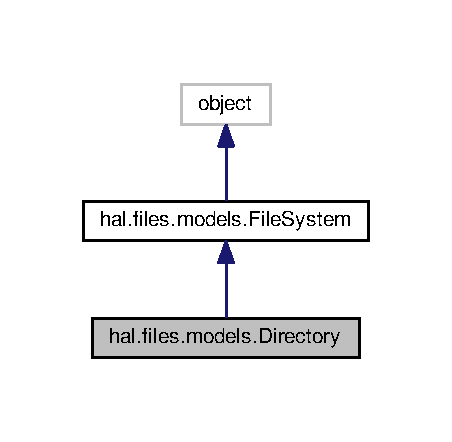
\includegraphics[width=217pt]{classhal_1_1files_1_1models_1_1_directory__inherit__graph}
\end{center}
\end{figure}


Collaboration diagram for hal.\+files.\+models.\+Directory\+:
\nopagebreak
\begin{figure}[H]
\begin{center}
\leavevmode
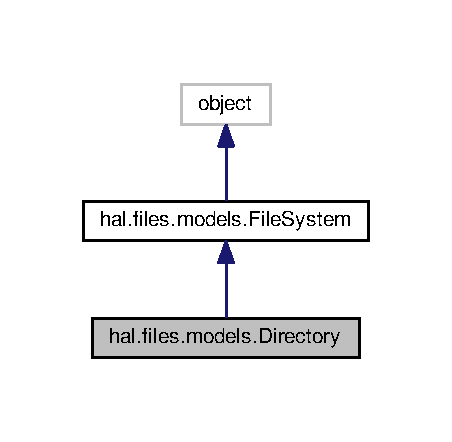
\includegraphics[width=217pt]{classhal_1_1files_1_1models_1_1_directory__coll__graph}
\end{center}
\end{figure}
\subsection*{Public Member Functions}
\begin{DoxyCompactItemize}
\item 
def \hyperlink{classhal_1_1files_1_1models_1_1_directory_ae4f13948eb8127b0c62f56d0ddf154b1}{\+\_\+\+\_\+init\+\_\+\+\_\+} (self, path)
\item 
def \hyperlink{classhal_1_1files_1_1models_1_1_directory_a58118af8552193237b38f7f341773707}{get\+\_\+path\+\_\+name} (self)
\item 
def \hyperlink{classhal_1_1files_1_1models_1_1_directory_a2a7a4af7d8d8d9e8e0d121ae9b673ce7}{is\+\_\+empty} (self)
\end{DoxyCompactItemize}
\subsection*{Static Public Member Functions}
\begin{DoxyCompactItemize}
\item 
def \hyperlink{classhal_1_1files_1_1models_1_1_directory_ac1f283483a8ae3cdc09634882be2e419}{create\+\_\+new} (path)
\end{DoxyCompactItemize}
\subsection*{Public Attributes}
\begin{DoxyCompactItemize}
\item 
{\bfseries name}\hypertarget{classhal_1_1files_1_1models_1_1_directory_a881eb92f96a89ccd626fb1c4be7da135}{}\label{classhal_1_1files_1_1models_1_1_directory_a881eb92f96a89ccd626fb1c4be7da135}

\end{DoxyCompactItemize}


\subsection{Constructor \& Destructor Documentation}
\index{hal\+::files\+::models\+::\+Directory@{hal\+::files\+::models\+::\+Directory}!\+\_\+\+\_\+init\+\_\+\+\_\+@{\+\_\+\+\_\+init\+\_\+\+\_\+}}
\index{\+\_\+\+\_\+init\+\_\+\+\_\+@{\+\_\+\+\_\+init\+\_\+\+\_\+}!hal\+::files\+::models\+::\+Directory@{hal\+::files\+::models\+::\+Directory}}
\subsubsection[{\texorpdfstring{\+\_\+\+\_\+init\+\_\+\+\_\+(self, path)}{__init__(self, path)}}]{\setlength{\rightskip}{0pt plus 5cm}def hal.\+files.\+models.\+Directory.\+\_\+\+\_\+init\+\_\+\+\_\+ (
\begin{DoxyParamCaption}
\item[{}]{self, }
\item[{}]{path}
\end{DoxyParamCaption}
)}\hypertarget{classhal_1_1files_1_1models_1_1_directory_ae4f13948eb8127b0c62f56d0ddf154b1}{}\label{classhal_1_1files_1_1models_1_1_directory_ae4f13948eb8127b0c62f56d0ddf154b1}
\begin{DoxyVerb}:param path: string
    Path to file
\end{DoxyVerb}
 

\subsection{Member Function Documentation}
\index{hal\+::files\+::models\+::\+Directory@{hal\+::files\+::models\+::\+Directory}!create\+\_\+new@{create\+\_\+new}}
\index{create\+\_\+new@{create\+\_\+new}!hal\+::files\+::models\+::\+Directory@{hal\+::files\+::models\+::\+Directory}}
\subsubsection[{\texorpdfstring{create\+\_\+new(path)}{create_new(path)}}]{\setlength{\rightskip}{0pt plus 5cm}def hal.\+files.\+models.\+Directory.\+create\+\_\+new (
\begin{DoxyParamCaption}
\item[{}]{path}
\end{DoxyParamCaption}
)\hspace{0.3cm}{\ttfamily [static]}}\hypertarget{classhal_1_1files_1_1models_1_1_directory_ac1f283483a8ae3cdc09634882be2e419}{}\label{classhal_1_1files_1_1models_1_1_directory_ac1f283483a8ae3cdc09634882be2e419}
\begin{DoxyVerb}:param path: string
    Path to directory to create
:return: void
    Creates new directory
\end{DoxyVerb}
 \index{hal\+::files\+::models\+::\+Directory@{hal\+::files\+::models\+::\+Directory}!get\+\_\+path\+\_\+name@{get\+\_\+path\+\_\+name}}
\index{get\+\_\+path\+\_\+name@{get\+\_\+path\+\_\+name}!hal\+::files\+::models\+::\+Directory@{hal\+::files\+::models\+::\+Directory}}
\subsubsection[{\texorpdfstring{get\+\_\+path\+\_\+name(self)}{get_path_name(self)}}]{\setlength{\rightskip}{0pt plus 5cm}def hal.\+files.\+models.\+Directory.\+get\+\_\+path\+\_\+name (
\begin{DoxyParamCaption}
\item[{}]{self}
\end{DoxyParamCaption}
)}\hypertarget{classhal_1_1files_1_1models_1_1_directory_a58118af8552193237b38f7f341773707}{}\label{classhal_1_1files_1_1models_1_1_directory_a58118af8552193237b38f7f341773707}
\begin{DoxyVerb}:return: tuple string, string
    Name of path, name of file (or folder)
\end{DoxyVerb}
 \index{hal\+::files\+::models\+::\+Directory@{hal\+::files\+::models\+::\+Directory}!is\+\_\+empty@{is\+\_\+empty}}
\index{is\+\_\+empty@{is\+\_\+empty}!hal\+::files\+::models\+::\+Directory@{hal\+::files\+::models\+::\+Directory}}
\subsubsection[{\texorpdfstring{is\+\_\+empty(self)}{is_empty(self)}}]{\setlength{\rightskip}{0pt plus 5cm}def hal.\+files.\+models.\+Directory.\+is\+\_\+empty (
\begin{DoxyParamCaption}
\item[{}]{self}
\end{DoxyParamCaption}
)}\hypertarget{classhal_1_1files_1_1models_1_1_directory_a2a7a4af7d8d8d9e8e0d121ae9b673ce7}{}\label{classhal_1_1files_1_1models_1_1_directory_a2a7a4af7d8d8d9e8e0d121ae9b673ce7}
\begin{DoxyVerb}:return: Bool
    True iff empty
\end{DoxyVerb}
 

The documentation for this class was generated from the following file\+:\begin{DoxyCompactItemize}
\item 
hal/files/models.\+py\end{DoxyCompactItemize}

\hypertarget{classhal_1_1files_1_1models_1_1_document}{}\section{hal.\+files.\+models.\+Document Class Reference}
\label{classhal_1_1files_1_1models_1_1_document}\index{hal.\+files.\+models.\+Document@{hal.\+files.\+models.\+Document}}


Inheritance diagram for hal.\+files.\+models.\+Document\+:\nopagebreak
\begin{figure}[H]
\begin{center}
\leavevmode
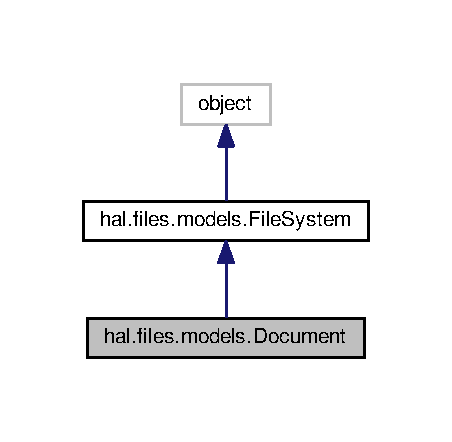
\includegraphics[width=217pt]{classhal_1_1files_1_1models_1_1_document__inherit__graph}
\end{center}
\end{figure}


Collaboration diagram for hal.\+files.\+models.\+Document\+:\nopagebreak
\begin{figure}[H]
\begin{center}
\leavevmode
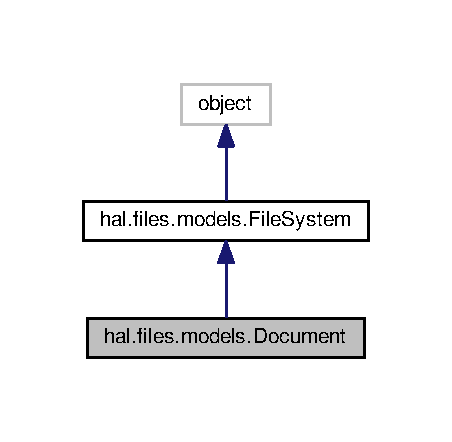
\includegraphics[width=217pt]{classhal_1_1files_1_1models_1_1_document__coll__graph}
\end{center}
\end{figure}
\subsection*{Public Member Functions}
\begin{DoxyCompactItemize}
\item 
def \hyperlink{classhal_1_1files_1_1models_1_1_document_a2080309a793ba5fe60aa26fcaf3c0bbd}{\+\_\+\+\_\+init\+\_\+\+\_\+} (self, path)
\item 
def \hyperlink{classhal_1_1files_1_1models_1_1_document_a157a403918f676d1bdaaa58177cafca2}{get\+\_\+path\+\_\+name} (self)
\item 
def \hyperlink{classhal_1_1files_1_1models_1_1_document_a6666175408a32f5a1cf700e0e0315c15}{is\+\_\+video} (self)
\item 
def \hyperlink{classhal_1_1files_1_1models_1_1_document_a6ec8b0654bc6ff54b82f3bacad4ceb1b}{is\+\_\+subtitle} (self)
\item 
def \hyperlink{classhal_1_1files_1_1models_1_1_document_aecb93cd7bde7e21fef16c50538451815}{is\+\_\+text} (self)
\item 
def \hyperlink{classhal_1_1files_1_1models_1_1_document_a56f51ccb5598448441cd681b95540ce5}{is\+\_\+image} (self)
\item 
def \hyperlink{classhal_1_1files_1_1models_1_1_document_ab9c88190355f8602dd4fcdb3f66d5c71}{is\+\_\+audio} (self)
\item 
def \hyperlink{classhal_1_1files_1_1models_1_1_document_acb08b90372387db6c0047f8f0e4aa23b}{is\+\_\+hidden} (self)
\end{DoxyCompactItemize}
\subsection*{Static Public Member Functions}
\begin{DoxyCompactItemize}
\item 
def \hyperlink{classhal_1_1files_1_1models_1_1_document_a667fad984369339c6c03f21a91394f54}{move\+\_\+file\+\_\+to\+\_\+directory} (file\+\_\+path, directory\+\_\+path)
\item 
def \hyperlink{classhal_1_1files_1_1models_1_1_document_ae1d5c82d81497dcea679f77bdbc84387}{move\+\_\+file\+\_\+to\+\_\+file} (old\+\_\+path, new\+\_\+path)
\item 
def \hyperlink{classhal_1_1files_1_1models_1_1_document_a7e506ca64800b613848c58338eecd077}{write\+\_\+data\+\_\+to\+\_\+file} (data, out\+\_\+file)
\item 
def \hyperlink{classhal_1_1files_1_1models_1_1_document_ade6b922c91273016659c2698031fc35e}{extract\+\_\+name\+\_\+extension} (file\+\_\+name)
\end{DoxyCompactItemize}
\subsection*{Public Attributes}
\begin{DoxyCompactItemize}
\item 
{\bfseries full\+\_\+name}\hypertarget{classhal_1_1files_1_1models_1_1_document_a001d1a849951ad3a43139b45a9f26bf4}{}\label{classhal_1_1files_1_1models_1_1_document_a001d1a849951ad3a43139b45a9f26bf4}

\item 
{\bfseries extension}\hypertarget{classhal_1_1files_1_1models_1_1_document_a6770905738040c9bcb052456bb41ce97}{}\label{classhal_1_1files_1_1models_1_1_document_a6770905738040c9bcb052456bb41ce97}

\end{DoxyCompactItemize}


\subsection{Constructor \& Destructor Documentation}
\index{hal\+::files\+::models\+::\+Document@{hal\+::files\+::models\+::\+Document}!\+\_\+\+\_\+init\+\_\+\+\_\+@{\+\_\+\+\_\+init\+\_\+\+\_\+}}
\index{\+\_\+\+\_\+init\+\_\+\+\_\+@{\+\_\+\+\_\+init\+\_\+\+\_\+}!hal\+::files\+::models\+::\+Document@{hal\+::files\+::models\+::\+Document}}
\subsubsection[{\texorpdfstring{\+\_\+\+\_\+init\+\_\+\+\_\+(self, path)}{__init__(self, path)}}]{\setlength{\rightskip}{0pt plus 5cm}def hal.\+files.\+models.\+Document.\+\_\+\+\_\+init\+\_\+\+\_\+ (
\begin{DoxyParamCaption}
\item[{}]{self, }
\item[{}]{path}
\end{DoxyParamCaption}
)}\hypertarget{classhal_1_1files_1_1models_1_1_document_a2080309a793ba5fe60aa26fcaf3c0bbd}{}\label{classhal_1_1files_1_1models_1_1_document_a2080309a793ba5fe60aa26fcaf3c0bbd}
\begin{DoxyVerb}:param path: string
    Path to file
\end{DoxyVerb}
 

\subsection{Member Function Documentation}
\index{hal\+::files\+::models\+::\+Document@{hal\+::files\+::models\+::\+Document}!extract\+\_\+name\+\_\+extension@{extract\+\_\+name\+\_\+extension}}
\index{extract\+\_\+name\+\_\+extension@{extract\+\_\+name\+\_\+extension}!hal\+::files\+::models\+::\+Document@{hal\+::files\+::models\+::\+Document}}
\subsubsection[{\texorpdfstring{extract\+\_\+name\+\_\+extension(file\+\_\+name)}{extract_name_extension(file_name)}}]{\setlength{\rightskip}{0pt plus 5cm}def hal.\+files.\+models.\+Document.\+extract\+\_\+name\+\_\+extension (
\begin{DoxyParamCaption}
\item[{}]{file\+\_\+name}
\end{DoxyParamCaption}
)\hspace{0.3cm}{\ttfamily [static]}}\hypertarget{classhal_1_1files_1_1models_1_1_document_ade6b922c91273016659c2698031fc35e}{}\label{classhal_1_1files_1_1models_1_1_document_ade6b922c91273016659c2698031fc35e}
\begin{DoxyVerb}:param file_name: string
    Name of file
:return: tuple string, string
    Name of file, extension of file
\end{DoxyVerb}
 \index{hal\+::files\+::models\+::\+Document@{hal\+::files\+::models\+::\+Document}!get\+\_\+path\+\_\+name@{get\+\_\+path\+\_\+name}}
\index{get\+\_\+path\+\_\+name@{get\+\_\+path\+\_\+name}!hal\+::files\+::models\+::\+Document@{hal\+::files\+::models\+::\+Document}}
\subsubsection[{\texorpdfstring{get\+\_\+path\+\_\+name(self)}{get_path_name(self)}}]{\setlength{\rightskip}{0pt plus 5cm}def hal.\+files.\+models.\+Document.\+get\+\_\+path\+\_\+name (
\begin{DoxyParamCaption}
\item[{}]{self}
\end{DoxyParamCaption}
)}\hypertarget{classhal_1_1files_1_1models_1_1_document_a157a403918f676d1bdaaa58177cafca2}{}\label{classhal_1_1files_1_1models_1_1_document_a157a403918f676d1bdaaa58177cafca2}
\begin{DoxyVerb}:return: tuple string, string
    Name of path, name of file (or folder)
\end{DoxyVerb}
 \index{hal\+::files\+::models\+::\+Document@{hal\+::files\+::models\+::\+Document}!is\+\_\+audio@{is\+\_\+audio}}
\index{is\+\_\+audio@{is\+\_\+audio}!hal\+::files\+::models\+::\+Document@{hal\+::files\+::models\+::\+Document}}
\subsubsection[{\texorpdfstring{is\+\_\+audio(self)}{is_audio(self)}}]{\setlength{\rightskip}{0pt plus 5cm}def hal.\+files.\+models.\+Document.\+is\+\_\+audio (
\begin{DoxyParamCaption}
\item[{}]{self}
\end{DoxyParamCaption}
)}\hypertarget{classhal_1_1files_1_1models_1_1_document_ab9c88190355f8602dd4fcdb3f66d5c71}{}\label{classhal_1_1files_1_1models_1_1_document_ab9c88190355f8602dd4fcdb3f66d5c71}
\begin{DoxyVerb}:return: True iff document is an audio.
\end{DoxyVerb}
 \index{hal\+::files\+::models\+::\+Document@{hal\+::files\+::models\+::\+Document}!is\+\_\+hidden@{is\+\_\+hidden}}
\index{is\+\_\+hidden@{is\+\_\+hidden}!hal\+::files\+::models\+::\+Document@{hal\+::files\+::models\+::\+Document}}
\subsubsection[{\texorpdfstring{is\+\_\+hidden(self)}{is_hidden(self)}}]{\setlength{\rightskip}{0pt plus 5cm}def hal.\+files.\+models.\+Document.\+is\+\_\+hidden (
\begin{DoxyParamCaption}
\item[{}]{self}
\end{DoxyParamCaption}
)}\hypertarget{classhal_1_1files_1_1models_1_1_document_acb08b90372387db6c0047f8f0e4aa23b}{}\label{classhal_1_1files_1_1models_1_1_document_acb08b90372387db6c0047f8f0e4aa23b}
\begin{DoxyVerb}:return: bool
    True iff path is hidden
\end{DoxyVerb}
 \index{hal\+::files\+::models\+::\+Document@{hal\+::files\+::models\+::\+Document}!is\+\_\+image@{is\+\_\+image}}
\index{is\+\_\+image@{is\+\_\+image}!hal\+::files\+::models\+::\+Document@{hal\+::files\+::models\+::\+Document}}
\subsubsection[{\texorpdfstring{is\+\_\+image(self)}{is_image(self)}}]{\setlength{\rightskip}{0pt plus 5cm}def hal.\+files.\+models.\+Document.\+is\+\_\+image (
\begin{DoxyParamCaption}
\item[{}]{self}
\end{DoxyParamCaption}
)}\hypertarget{classhal_1_1files_1_1models_1_1_document_a56f51ccb5598448441cd681b95540ce5}{}\label{classhal_1_1files_1_1models_1_1_document_a56f51ccb5598448441cd681b95540ce5}
\begin{DoxyVerb}:return: True iff document is an image.
\end{DoxyVerb}
 \index{hal\+::files\+::models\+::\+Document@{hal\+::files\+::models\+::\+Document}!is\+\_\+subtitle@{is\+\_\+subtitle}}
\index{is\+\_\+subtitle@{is\+\_\+subtitle}!hal\+::files\+::models\+::\+Document@{hal\+::files\+::models\+::\+Document}}
\subsubsection[{\texorpdfstring{is\+\_\+subtitle(self)}{is_subtitle(self)}}]{\setlength{\rightskip}{0pt plus 5cm}def hal.\+files.\+models.\+Document.\+is\+\_\+subtitle (
\begin{DoxyParamCaption}
\item[{}]{self}
\end{DoxyParamCaption}
)}\hypertarget{classhal_1_1files_1_1models_1_1_document_a6ec8b0654bc6ff54b82f3bacad4ceb1b}{}\label{classhal_1_1files_1_1models_1_1_document_a6ec8b0654bc6ff54b82f3bacad4ceb1b}
\begin{DoxyVerb}:return: True iff document is a subtitle.
\end{DoxyVerb}
 \index{hal\+::files\+::models\+::\+Document@{hal\+::files\+::models\+::\+Document}!is\+\_\+text@{is\+\_\+text}}
\index{is\+\_\+text@{is\+\_\+text}!hal\+::files\+::models\+::\+Document@{hal\+::files\+::models\+::\+Document}}
\subsubsection[{\texorpdfstring{is\+\_\+text(self)}{is_text(self)}}]{\setlength{\rightskip}{0pt plus 5cm}def hal.\+files.\+models.\+Document.\+is\+\_\+text (
\begin{DoxyParamCaption}
\item[{}]{self}
\end{DoxyParamCaption}
)}\hypertarget{classhal_1_1files_1_1models_1_1_document_aecb93cd7bde7e21fef16c50538451815}{}\label{classhal_1_1files_1_1models_1_1_document_aecb93cd7bde7e21fef16c50538451815}
\begin{DoxyVerb}:return: True iff document is a text file.
\end{DoxyVerb}
 \index{hal\+::files\+::models\+::\+Document@{hal\+::files\+::models\+::\+Document}!is\+\_\+video@{is\+\_\+video}}
\index{is\+\_\+video@{is\+\_\+video}!hal\+::files\+::models\+::\+Document@{hal\+::files\+::models\+::\+Document}}
\subsubsection[{\texorpdfstring{is\+\_\+video(self)}{is_video(self)}}]{\setlength{\rightskip}{0pt plus 5cm}def hal.\+files.\+models.\+Document.\+is\+\_\+video (
\begin{DoxyParamCaption}
\item[{}]{self}
\end{DoxyParamCaption}
)}\hypertarget{classhal_1_1files_1_1models_1_1_document_a6666175408a32f5a1cf700e0e0315c15}{}\label{classhal_1_1files_1_1models_1_1_document_a6666175408a32f5a1cf700e0e0315c15}
\begin{DoxyVerb}:return: True iff document is a video.
\end{DoxyVerb}
 \index{hal\+::files\+::models\+::\+Document@{hal\+::files\+::models\+::\+Document}!move\+\_\+file\+\_\+to\+\_\+directory@{move\+\_\+file\+\_\+to\+\_\+directory}}
\index{move\+\_\+file\+\_\+to\+\_\+directory@{move\+\_\+file\+\_\+to\+\_\+directory}!hal\+::files\+::models\+::\+Document@{hal\+::files\+::models\+::\+Document}}
\subsubsection[{\texorpdfstring{move\+\_\+file\+\_\+to\+\_\+directory(file\+\_\+path, directory\+\_\+path)}{move_file_to_directory(file_path, directory_path)}}]{\setlength{\rightskip}{0pt plus 5cm}def hal.\+files.\+models.\+Document.\+move\+\_\+file\+\_\+to\+\_\+directory (
\begin{DoxyParamCaption}
\item[{}]{file\+\_\+path, }
\item[{}]{directory\+\_\+path}
\end{DoxyParamCaption}
)\hspace{0.3cm}{\ttfamily [static]}}\hypertarget{classhal_1_1files_1_1models_1_1_document_a667fad984369339c6c03f21a91394f54}{}\label{classhal_1_1files_1_1models_1_1_document_a667fad984369339c6c03f21a91394f54}
\begin{DoxyVerb}:param file_path: string
    Path to file to move
:param directory_path: string
    Path to target directory where to move file
:return: void
    Move file to given directory
\end{DoxyVerb}
 \index{hal\+::files\+::models\+::\+Document@{hal\+::files\+::models\+::\+Document}!move\+\_\+file\+\_\+to\+\_\+file@{move\+\_\+file\+\_\+to\+\_\+file}}
\index{move\+\_\+file\+\_\+to\+\_\+file@{move\+\_\+file\+\_\+to\+\_\+file}!hal\+::files\+::models\+::\+Document@{hal\+::files\+::models\+::\+Document}}
\subsubsection[{\texorpdfstring{move\+\_\+file\+\_\+to\+\_\+file(old\+\_\+path, new\+\_\+path)}{move_file_to_file(old_path, new_path)}}]{\setlength{\rightskip}{0pt plus 5cm}def hal.\+files.\+models.\+Document.\+move\+\_\+file\+\_\+to\+\_\+file (
\begin{DoxyParamCaption}
\item[{}]{old\+\_\+path, }
\item[{}]{new\+\_\+path}
\end{DoxyParamCaption}
)\hspace{0.3cm}{\ttfamily [static]}}\hypertarget{classhal_1_1files_1_1models_1_1_document_ae1d5c82d81497dcea679f77bdbc84387}{}\label{classhal_1_1files_1_1models_1_1_document_ae1d5c82d81497dcea679f77bdbc84387}
\begin{DoxyVerb}:param old_path: string
    Old path of file to move
:param new_path: string
    New path (location) of file
:return: void
    Move file from old location to new one
\end{DoxyVerb}
 \index{hal\+::files\+::models\+::\+Document@{hal\+::files\+::models\+::\+Document}!write\+\_\+data\+\_\+to\+\_\+file@{write\+\_\+data\+\_\+to\+\_\+file}}
\index{write\+\_\+data\+\_\+to\+\_\+file@{write\+\_\+data\+\_\+to\+\_\+file}!hal\+::files\+::models\+::\+Document@{hal\+::files\+::models\+::\+Document}}
\subsubsection[{\texorpdfstring{write\+\_\+data\+\_\+to\+\_\+file(data, out\+\_\+file)}{write_data_to_file(data, out_file)}}]{\setlength{\rightskip}{0pt plus 5cm}def hal.\+files.\+models.\+Document.\+write\+\_\+data\+\_\+to\+\_\+file (
\begin{DoxyParamCaption}
\item[{}]{data, }
\item[{}]{out\+\_\+file}
\end{DoxyParamCaption}
)\hspace{0.3cm}{\ttfamily [static]}}\hypertarget{classhal_1_1files_1_1models_1_1_document_a7e506ca64800b613848c58338eecd077}{}\label{classhal_1_1files_1_1models_1_1_document_a7e506ca64800b613848c58338eecd077}
\begin{DoxyVerb}:param data: string
    Data to write to file.
:param out_file: string
    Path to output file.
:return: void
    Writes given data to given path file.
\end{DoxyVerb}
 

The documentation for this class was generated from the following file\+:\begin{DoxyCompactItemize}
\item 
/home/stefano/\+Coding/\+Python/projects/pyhal/hal/files/models.\+py\end{DoxyCompactItemize}

\hypertarget{classhal_1_1maths_1_1crypt_1_1_dsa}{}\section{hal.\+maths.\+crypt.\+Dsa Class Reference}
\label{classhal_1_1maths_1_1crypt_1_1_dsa}\index{hal.\+maths.\+crypt.\+Dsa@{hal.\+maths.\+crypt.\+Dsa}}


Inheritance diagram for hal.\+maths.\+crypt.\+Dsa\+:\nopagebreak
\begin{figure}[H]
\begin{center}
\leavevmode
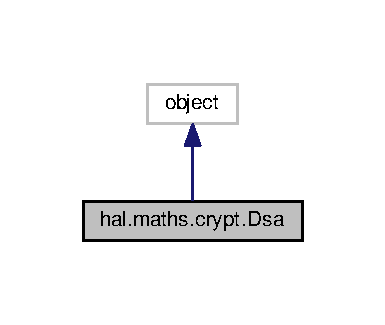
\includegraphics[width=185pt]{classhal_1_1maths_1_1crypt_1_1_dsa__inherit__graph}
\end{center}
\end{figure}


Collaboration diagram for hal.\+maths.\+crypt.\+Dsa\+:\nopagebreak
\begin{figure}[H]
\begin{center}
\leavevmode
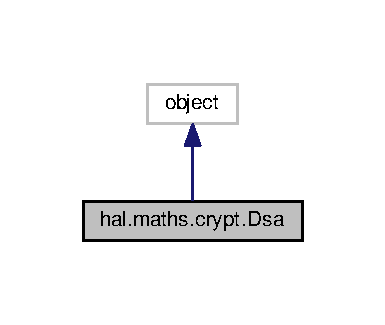
\includegraphics[width=185pt]{classhal_1_1maths_1_1crypt_1_1_dsa__coll__graph}
\end{center}
\end{figure}
\subsection*{Public Member Functions}
\begin{DoxyCompactItemize}
\item 
def {\bfseries \+\_\+\+\_\+init\+\_\+\+\_\+} (self, string)\hypertarget{classhal_1_1maths_1_1crypt_1_1_dsa_a127aadb2c49476c4ffc47537beb0a47f}{}\label{classhal_1_1maths_1_1crypt_1_1_dsa_a127aadb2c49476c4ffc47537beb0a47f}

\item 
def \hyperlink{classhal_1_1maths_1_1crypt_1_1_dsa_ab571cc724b6bd76e1001d9d449cb6c61}{hash} (self)
\end{DoxyCompactItemize}
\subsection*{Public Attributes}
\begin{DoxyCompactItemize}
\item 
{\bfseries plain}\hypertarget{classhal_1_1maths_1_1crypt_1_1_dsa_a8fddacfaa756e3400dd60e62edecae5d}{}\label{classhal_1_1maths_1_1crypt_1_1_dsa_a8fddacfaa756e3400dd60e62edecae5d}

\item 
{\bfseries hashed}\hypertarget{classhal_1_1maths_1_1crypt_1_1_dsa_af05db55c1f6ebca07b027397a8f494dd}{}\label{classhal_1_1maths_1_1crypt_1_1_dsa_af05db55c1f6ebca07b027397a8f494dd}

\end{DoxyCompactItemize}


\subsection{Detailed Description}
\begin{DoxyVerb}dsa hash \end{DoxyVerb}
 

\subsection{Member Function Documentation}
\index{hal\+::maths\+::crypt\+::\+Dsa@{hal\+::maths\+::crypt\+::\+Dsa}!hash@{hash}}
\index{hash@{hash}!hal\+::maths\+::crypt\+::\+Dsa@{hal\+::maths\+::crypt\+::\+Dsa}}
\subsubsection[{\texorpdfstring{hash(self)}{hash(self)}}]{\setlength{\rightskip}{0pt plus 5cm}def hal.\+maths.\+crypt.\+Dsa.\+hash (
\begin{DoxyParamCaption}
\item[{}]{self}
\end{DoxyParamCaption}
)}\hypertarget{classhal_1_1maths_1_1crypt_1_1_dsa_ab571cc724b6bd76e1001d9d449cb6c61}{}\label{classhal_1_1maths_1_1crypt_1_1_dsa_ab571cc724b6bd76e1001d9d449cb6c61}
\begin{DoxyVerb}:return: hash plaintext
\end{DoxyVerb}
 

The documentation for this class was generated from the following file\+:\begin{DoxyCompactItemize}
\item 
/home/stefano/\+Coding/\+Python/projects/pyhal/hal/maths/crypt.\+py\end{DoxyCompactItemize}

\hypertarget{classhal_1_1maths_1_1maths_1_1_eight_queen}{}\section{hal.\+maths.\+maths.\+Eight\+Queen Class Reference}
\label{classhal_1_1maths_1_1maths_1_1_eight_queen}\index{hal.\+maths.\+maths.\+Eight\+Queen@{hal.\+maths.\+maths.\+Eight\+Queen}}


Inheritance diagram for hal.\+maths.\+maths.\+Eight\+Queen\+:
\nopagebreak
\begin{figure}[H]
\begin{center}
\leavevmode
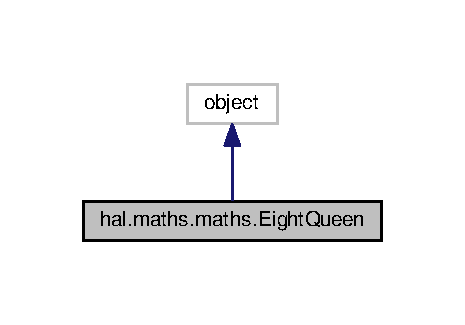
\includegraphics[width=223pt]{classhal_1_1maths_1_1maths_1_1_eight_queen__inherit__graph}
\end{center}
\end{figure}


Collaboration diagram for hal.\+maths.\+maths.\+Eight\+Queen\+:
\nopagebreak
\begin{figure}[H]
\begin{center}
\leavevmode
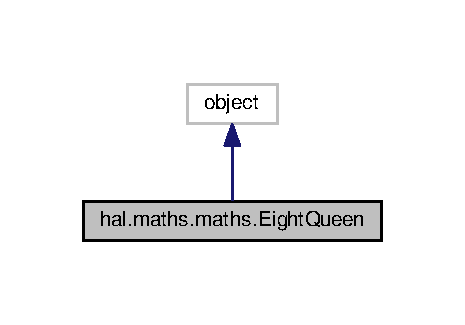
\includegraphics[width=223pt]{classhal_1_1maths_1_1maths_1_1_eight_queen__coll__graph}
\end{center}
\end{figure}
\subsection*{Public Member Functions}
\begin{DoxyCompactItemize}
\item 
def {\bfseries \+\_\+\+\_\+init\+\_\+\+\_\+} (self, board\+\_\+size)\hypertarget{classhal_1_1maths_1_1maths_1_1_eight_queen_a71642e4346629fda32e51c647c28fa3f}{}\label{classhal_1_1maths_1_1maths_1_1_eight_queen_a71642e4346629fda32e51c647c28fa3f}

\item 
def {\bfseries under\+\_\+attack} (self, col, queens)\hypertarget{classhal_1_1maths_1_1maths_1_1_eight_queen_a8e7e221caa5ac408c49d69116076595e}{}\label{classhal_1_1maths_1_1maths_1_1_eight_queen_a8e7e221caa5ac408c49d69116076595e}

\item 
def {\bfseries solve} (self, n)\hypertarget{classhal_1_1maths_1_1maths_1_1_eight_queen_a8147e8ea2dabfa44b3c8d13e04d7b529}{}\label{classhal_1_1maths_1_1maths_1_1_eight_queen_a8147e8ea2dabfa44b3c8d13e04d7b529}

\end{DoxyCompactItemize}
\subsection*{Public Attributes}
\begin{DoxyCompactItemize}
\item 
{\bfseries board\+\_\+size}\hypertarget{classhal_1_1maths_1_1maths_1_1_eight_queen_a8d242fe77a100b25c6ab6e861069623b}{}\label{classhal_1_1maths_1_1maths_1_1_eight_queen_a8d242fe77a100b25c6ab6e861069623b}

\end{DoxyCompactItemize}


\subsection{Detailed Description}
\begin{DoxyVerb}8 queen problem solver \end{DoxyVerb}
 

The documentation for this class was generated from the following file\+:\begin{DoxyCompactItemize}
\item 
hal/maths/maths.\+py\end{DoxyCompactItemize}

\hypertarget{classhal_1_1profile_1_1performance_1_1_eight_queen_test}{}\section{hal.\+profile.\+performance.\+Eight\+Queen\+Test Class Reference}
\label{classhal_1_1profile_1_1performance_1_1_eight_queen_test}\index{hal.\+profile.\+performance.\+Eight\+Queen\+Test@{hal.\+profile.\+performance.\+Eight\+Queen\+Test}}


Inheritance diagram for hal.\+profile.\+performance.\+Eight\+Queen\+Test\+:\nopagebreak
\begin{figure}[H]
\begin{center}
\leavevmode
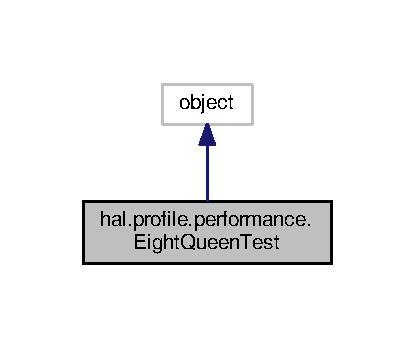
\includegraphics[width=199pt]{classhal_1_1profile_1_1performance_1_1_eight_queen_test__inherit__graph}
\end{center}
\end{figure}


Collaboration diagram for hal.\+profile.\+performance.\+Eight\+Queen\+Test\+:\nopagebreak
\begin{figure}[H]
\begin{center}
\leavevmode
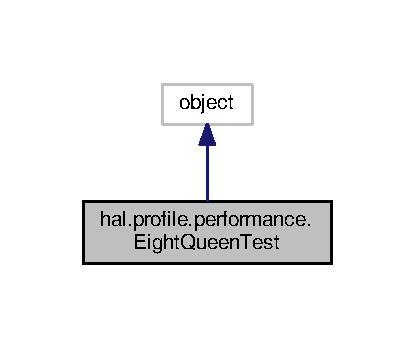
\includegraphics[width=199pt]{classhal_1_1profile_1_1performance_1_1_eight_queen_test__coll__graph}
\end{center}
\end{figure}
\subsection*{Public Member Functions}
\begin{DoxyCompactItemize}
\item 
def {\bfseries \+\_\+\+\_\+init\+\_\+\+\_\+} (self, size)\hypertarget{classhal_1_1profile_1_1performance_1_1_eight_queen_test_aff4c0640adbaf044ee1a2f1d20480647}{}\label{classhal_1_1profile_1_1performance_1_1_eight_queen_test_aff4c0640adbaf044ee1a2f1d20480647}

\item 
def \hyperlink{classhal_1_1profile_1_1performance_1_1_eight_queen_test_a39eed18e353b03f5ab738496826544f0}{update\+\_\+std\+\_\+out\+\_\+and\+\_\+log} (self, string)
\item 
def {\bfseries start} (self)\hypertarget{classhal_1_1profile_1_1performance_1_1_eight_queen_test_aae7444405fb2139e4261aa639e27892f}{}\label{classhal_1_1profile_1_1performance_1_1_eight_queen_test_aae7444405fb2139e4261aa639e27892f}

\end{DoxyCompactItemize}
\subsection*{Static Public Member Functions}
\begin{DoxyCompactItemize}
\item 
def \hyperlink{classhal_1_1profile_1_1performance_1_1_eight_queen_test_a981be709c0e10f0098a8c58af1929746}{welcome} ()
\item 
def \hyperlink{classhal_1_1profile_1_1performance_1_1_eight_queen_test_a570aa1a773c9d24cca31e6a42e852fd4}{introduction} ()
\item 
def \hyperlink{classhal_1_1profile_1_1performance_1_1_eight_queen_test_a1830ea92c280cbd39a65c7fc36176e89}{run\+\_\+test\+\_\+with\+\_\+size} (size)
\end{DoxyCompactItemize}
\subsection*{Public Attributes}
\begin{DoxyCompactItemize}
\item 
{\bfseries size}\hypertarget{classhal_1_1profile_1_1performance_1_1_eight_queen_test_afefe08b8ae5a8a787f867d97cc2d6ad4}{}\label{classhal_1_1profile_1_1performance_1_1_eight_queen_test_afefe08b8ae5a8a787f867d97cc2d6ad4}

\item 
{\bfseries benchmark}\hypertarget{classhal_1_1profile_1_1performance_1_1_eight_queen_test_a537a15f71e5641f883b9e54acd04d163}{}\label{classhal_1_1profile_1_1performance_1_1_eight_queen_test_a537a15f71e5641f883b9e54acd04d163}

\end{DoxyCompactItemize}


\subsection{Detailed Description}
\begin{DoxyVerb}Test CPU by solving eight-queen problem \end{DoxyVerb}
 

\subsection{Member Function Documentation}
\index{hal\+::profile\+::performance\+::\+Eight\+Queen\+Test@{hal\+::profile\+::performance\+::\+Eight\+Queen\+Test}!introduction@{introduction}}
\index{introduction@{introduction}!hal\+::profile\+::performance\+::\+Eight\+Queen\+Test@{hal\+::profile\+::performance\+::\+Eight\+Queen\+Test}}
\subsubsection[{\texorpdfstring{introduction()}{introduction()}}]{\setlength{\rightskip}{0pt plus 5cm}def hal.\+profile.\+performance.\+Eight\+Queen\+Test.\+introduction (
\begin{DoxyParamCaption}
{}
\end{DoxyParamCaption}
)\hspace{0.3cm}{\ttfamily [static]}}\hypertarget{classhal_1_1profile_1_1performance_1_1_eight_queen_test_a570aa1a773c9d24cca31e6a42e852fd4}{}\label{classhal_1_1profile_1_1performance_1_1_eight_queen_test_a570aa1a773c9d24cca31e6a42e852fd4}
\begin{DoxyVerb}:return: string
    Welcomes user to this test sessions
\end{DoxyVerb}
 \index{hal\+::profile\+::performance\+::\+Eight\+Queen\+Test@{hal\+::profile\+::performance\+::\+Eight\+Queen\+Test}!run\+\_\+test\+\_\+with\+\_\+size@{run\+\_\+test\+\_\+with\+\_\+size}}
\index{run\+\_\+test\+\_\+with\+\_\+size@{run\+\_\+test\+\_\+with\+\_\+size}!hal\+::profile\+::performance\+::\+Eight\+Queen\+Test@{hal\+::profile\+::performance\+::\+Eight\+Queen\+Test}}
\subsubsection[{\texorpdfstring{run\+\_\+test\+\_\+with\+\_\+size(size)}{run_test_with_size(size)}}]{\setlength{\rightskip}{0pt plus 5cm}def hal.\+profile.\+performance.\+Eight\+Queen\+Test.\+run\+\_\+test\+\_\+with\+\_\+size (
\begin{DoxyParamCaption}
\item[{}]{size}
\end{DoxyParamCaption}
)\hspace{0.3cm}{\ttfamily [static]}}\hypertarget{classhal_1_1profile_1_1performance_1_1_eight_queen_test_a1830ea92c280cbd39a65c7fc36176e89}{}\label{classhal_1_1profile_1_1performance_1_1_eight_queen_test_a1830ea92c280cbd39a65c7fc36176e89}
\begin{DoxyVerb}:param size: int
    Number of rows in grid
:return: int
    Time to solve problem with given size
\end{DoxyVerb}
 \index{hal\+::profile\+::performance\+::\+Eight\+Queen\+Test@{hal\+::profile\+::performance\+::\+Eight\+Queen\+Test}!update\+\_\+std\+\_\+out\+\_\+and\+\_\+log@{update\+\_\+std\+\_\+out\+\_\+and\+\_\+log}}
\index{update\+\_\+std\+\_\+out\+\_\+and\+\_\+log@{update\+\_\+std\+\_\+out\+\_\+and\+\_\+log}!hal\+::profile\+::performance\+::\+Eight\+Queen\+Test@{hal\+::profile\+::performance\+::\+Eight\+Queen\+Test}}
\subsubsection[{\texorpdfstring{update\+\_\+std\+\_\+out\+\_\+and\+\_\+log(self, string)}{update_std_out_and_log(self, string)}}]{\setlength{\rightskip}{0pt plus 5cm}def hal.\+profile.\+performance.\+Eight\+Queen\+Test.\+update\+\_\+std\+\_\+out\+\_\+and\+\_\+log (
\begin{DoxyParamCaption}
\item[{}]{self, }
\item[{}]{string}
\end{DoxyParamCaption}
)}\hypertarget{classhal_1_1profile_1_1performance_1_1_eight_queen_test_a39eed18e353b03f5ab738496826544f0}{}\label{classhal_1_1profile_1_1performance_1_1_eight_queen_test_a39eed18e353b03f5ab738496826544f0}
\begin{DoxyVerb}:param string: string
    Stuff to print
:return: void
    Prints to stdout and updates log
\end{DoxyVerb}
 \index{hal\+::profile\+::performance\+::\+Eight\+Queen\+Test@{hal\+::profile\+::performance\+::\+Eight\+Queen\+Test}!welcome@{welcome}}
\index{welcome@{welcome}!hal\+::profile\+::performance\+::\+Eight\+Queen\+Test@{hal\+::profile\+::performance\+::\+Eight\+Queen\+Test}}
\subsubsection[{\texorpdfstring{welcome()}{welcome()}}]{\setlength{\rightskip}{0pt plus 5cm}def hal.\+profile.\+performance.\+Eight\+Queen\+Test.\+welcome (
\begin{DoxyParamCaption}
{}
\end{DoxyParamCaption}
)\hspace{0.3cm}{\ttfamily [static]}}\hypertarget{classhal_1_1profile_1_1performance_1_1_eight_queen_test_a981be709c0e10f0098a8c58af1929746}{}\label{classhal_1_1profile_1_1performance_1_1_eight_queen_test_a981be709c0e10f0098a8c58af1929746}
\begin{DoxyVerb}:return: string
    Welcomes user to this test sessions
\end{DoxyVerb}
 

The documentation for this class was generated from the following file\+:\begin{DoxyCompactItemize}
\item 
/home/stefano/\+Coding/\+Python/projects/pyhal/hal/profile/performance.\+py\end{DoxyCompactItemize}

\hypertarget{classhal_1_1files_1_1models_1_1_file_system}{}\section{hal.\+files.\+models.\+File\+System Class Reference}
\label{classhal_1_1files_1_1models_1_1_file_system}\index{hal.\+files.\+models.\+File\+System@{hal.\+files.\+models.\+File\+System}}


Inheritance diagram for hal.\+files.\+models.\+File\+System\+:\nopagebreak
\begin{figure}[H]
\begin{center}
\leavevmode
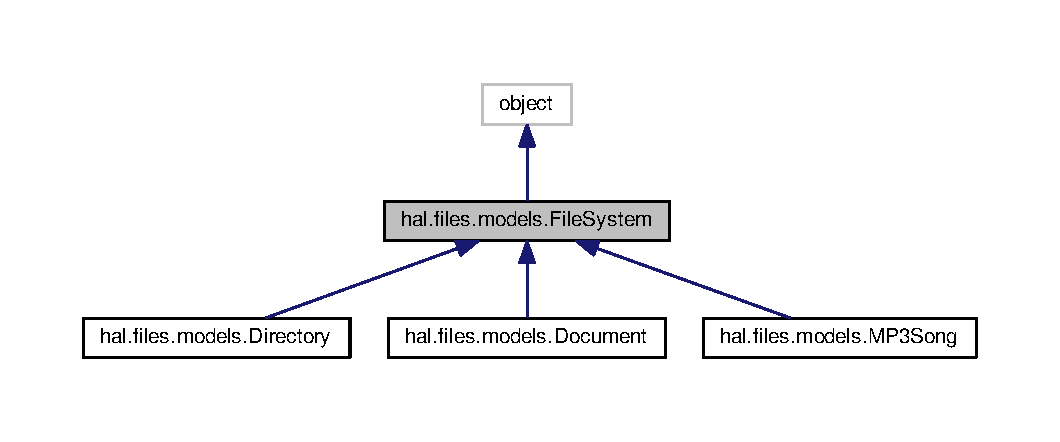
\includegraphics[width=350pt]{classhal_1_1files_1_1models_1_1_file_system__inherit__graph}
\end{center}
\end{figure}


Collaboration diagram for hal.\+files.\+models.\+File\+System\+:\nopagebreak
\begin{figure}[H]
\begin{center}
\leavevmode
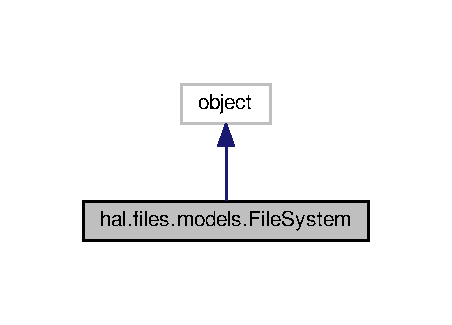
\includegraphics[width=217pt]{classhal_1_1files_1_1models_1_1_file_system__coll__graph}
\end{center}
\end{figure}
\subsection*{Public Member Functions}
\begin{DoxyCompactItemize}
\item 
def \hyperlink{classhal_1_1files_1_1models_1_1_file_system_a17bf22e8739c0abe81a1736115ff6778}{\+\_\+\+\_\+init\+\_\+\+\_\+} (self, path)
\item 
def \hyperlink{classhal_1_1files_1_1models_1_1_file_system_a7b176e08ad6531bcc9caa04c44df1944}{is\+\_\+archive\+\_\+mac} (self)
\item 
def \hyperlink{classhal_1_1files_1_1models_1_1_file_system_a073400419be263c865c0971136d2898b}{is\+\_\+russian} (self)
\item 
def \hyperlink{classhal_1_1files_1_1models_1_1_file_system_a98912c19e86d13c67b0a9bb70682026c}{trash} (self)
\item 
def \hyperlink{classhal_1_1files_1_1models_1_1_file_system_a3388d434e8ae2be2f2b7b9a227ac418e}{rename} (self, new\+\_\+path)
\end{DoxyCompactItemize}
\subsection*{Static Public Member Functions}
\begin{DoxyCompactItemize}
\item 
def \hyperlink{classhal_1_1files_1_1models_1_1_file_system_a7fe20d282e84a1ad292f7e04de6d335d}{fix\+\_\+raw\+\_\+path} (path)
\item 
def \hyperlink{classhal_1_1files_1_1models_1_1_file_system_af473fc3f0450ffe57c2484fd76d3a40d}{remove\+\_\+year} (name)
\item 
def \hyperlink{classhal_1_1files_1_1models_1_1_file_system_ab97d14ce121829510e40c3f052c176df}{remove\+\_\+brackets} (name)
\item 
def \hyperlink{classhal_1_1files_1_1models_1_1_file_system_a809f1abc2282567f89f809a510e7d665}{extract\+\_\+name\+\_\+max\+\_\+chars} (name, max\+\_\+chars=64, blank=\char`\"{} \char`\"{})
\item 
def \hyperlink{classhal_1_1files_1_1models_1_1_file_system_a81206c773e9176fb2c0537a731381b7a}{prettify} (name, bad\+\_\+chars=B\+A\+D\+\_\+\+C\+H\+A\+RS, r=\char`\"{} \char`\"{})
\item 
def \hyperlink{classhal_1_1files_1_1models_1_1_file_system_a60f66aeec22d00b67067f3527d06db74}{ls\+\_\+dir} (path, include\+\_\+hidden=False)
\item 
def \hyperlink{classhal_1_1files_1_1models_1_1_file_system_a2df7cb545b239ccb239b71f808ce5808}{ls\+\_\+recurse} (path, include\+\_\+hidden=False)
\item 
def \hyperlink{classhal_1_1files_1_1models_1_1_file_system_aaf2fadb1bb388e4b565da0db6823f4f5}{ls} (path, recurse, include\+\_\+hidden=False)
\end{DoxyCompactItemize}
\subsection*{Public Attributes}
\begin{DoxyCompactItemize}
\item 
{\bfseries path}\hypertarget{classhal_1_1files_1_1models_1_1_file_system_a261fa17468126979cedf206b69a1d071}{}\label{classhal_1_1files_1_1models_1_1_file_system_a261fa17468126979cedf206b69a1d071}

\end{DoxyCompactItemize}


\subsection{Constructor \& Destructor Documentation}
\index{hal\+::files\+::models\+::\+File\+System@{hal\+::files\+::models\+::\+File\+System}!\+\_\+\+\_\+init\+\_\+\+\_\+@{\+\_\+\+\_\+init\+\_\+\+\_\+}}
\index{\+\_\+\+\_\+init\+\_\+\+\_\+@{\+\_\+\+\_\+init\+\_\+\+\_\+}!hal\+::files\+::models\+::\+File\+System@{hal\+::files\+::models\+::\+File\+System}}
\subsubsection[{\texorpdfstring{\+\_\+\+\_\+init\+\_\+\+\_\+(self, path)}{__init__(self, path)}}]{\setlength{\rightskip}{0pt plus 5cm}def hal.\+files.\+models.\+File\+System.\+\_\+\+\_\+init\+\_\+\+\_\+ (
\begin{DoxyParamCaption}
\item[{}]{self, }
\item[{}]{path}
\end{DoxyParamCaption}
)}\hypertarget{classhal_1_1files_1_1models_1_1_file_system_a17bf22e8739c0abe81a1736115ff6778}{}\label{classhal_1_1files_1_1models_1_1_file_system_a17bf22e8739c0abe81a1736115ff6778}
\begin{DoxyVerb}:param path: string
    Path to file
\end{DoxyVerb}
 

\subsection{Member Function Documentation}
\index{hal\+::files\+::models\+::\+File\+System@{hal\+::files\+::models\+::\+File\+System}!extract\+\_\+name\+\_\+max\+\_\+chars@{extract\+\_\+name\+\_\+max\+\_\+chars}}
\index{extract\+\_\+name\+\_\+max\+\_\+chars@{extract\+\_\+name\+\_\+max\+\_\+chars}!hal\+::files\+::models\+::\+File\+System@{hal\+::files\+::models\+::\+File\+System}}
\subsubsection[{\texorpdfstring{extract\+\_\+name\+\_\+max\+\_\+chars(name, max\+\_\+chars=64, blank="" "")}{extract_name_max_chars(name, max_chars=64, blank=" ")}}]{\setlength{\rightskip}{0pt plus 5cm}def hal.\+files.\+models.\+File\+System.\+extract\+\_\+name\+\_\+max\+\_\+chars (
\begin{DoxyParamCaption}
\item[{}]{name, }
\item[{}]{max\+\_\+chars = {\ttfamily 64}, }
\item[{}]{blank = {\ttfamily \char`\"{}~\char`\"{}}}
\end{DoxyParamCaption}
)\hspace{0.3cm}{\ttfamily [static]}}\hypertarget{classhal_1_1files_1_1models_1_1_file_system_a809f1abc2282567f89f809a510e7d665}{}\label{classhal_1_1files_1_1models_1_1_file_system_a809f1abc2282567f89f809a510e7d665}
\begin{DoxyVerb}:param name: string
    Name to edit
:param max_chars: int
    Maximum chars of new name
:param blank: string
    Char that represents the blank between words.
:return: string
    Name edited to contain at most max_chars (truncate to nearest word)
\end{DoxyVerb}
 \index{hal\+::files\+::models\+::\+File\+System@{hal\+::files\+::models\+::\+File\+System}!fix\+\_\+raw\+\_\+path@{fix\+\_\+raw\+\_\+path}}
\index{fix\+\_\+raw\+\_\+path@{fix\+\_\+raw\+\_\+path}!hal\+::files\+::models\+::\+File\+System@{hal\+::files\+::models\+::\+File\+System}}
\subsubsection[{\texorpdfstring{fix\+\_\+raw\+\_\+path(path)}{fix_raw_path(path)}}]{\setlength{\rightskip}{0pt plus 5cm}def hal.\+files.\+models.\+File\+System.\+fix\+\_\+raw\+\_\+path (
\begin{DoxyParamCaption}
\item[{}]{path}
\end{DoxyParamCaption}
)\hspace{0.3cm}{\ttfamily [static]}}\hypertarget{classhal_1_1files_1_1models_1_1_file_system_a7fe20d282e84a1ad292f7e04de6d335d}{}\label{classhal_1_1files_1_1models_1_1_file_system_a7fe20d282e84a1ad292f7e04de6d335d}
\begin{DoxyVerb}:param path: string
    Path to fix
:return: string
    Right path
\end{DoxyVerb}
 \index{hal\+::files\+::models\+::\+File\+System@{hal\+::files\+::models\+::\+File\+System}!is\+\_\+archive\+\_\+mac@{is\+\_\+archive\+\_\+mac}}
\index{is\+\_\+archive\+\_\+mac@{is\+\_\+archive\+\_\+mac}!hal\+::files\+::models\+::\+File\+System@{hal\+::files\+::models\+::\+File\+System}}
\subsubsection[{\texorpdfstring{is\+\_\+archive\+\_\+mac(self)}{is_archive_mac(self)}}]{\setlength{\rightskip}{0pt plus 5cm}def hal.\+files.\+models.\+File\+System.\+is\+\_\+archive\+\_\+mac (
\begin{DoxyParamCaption}
\item[{}]{self}
\end{DoxyParamCaption}
)}\hypertarget{classhal_1_1files_1_1models_1_1_file_system_a7b176e08ad6531bcc9caa04c44df1944}{}\label{classhal_1_1files_1_1models_1_1_file_system_a7b176e08ad6531bcc9caa04c44df1944}
\begin{DoxyVerb}:return: True iff document is an MACOSX archive.
\end{DoxyVerb}
 \index{hal\+::files\+::models\+::\+File\+System@{hal\+::files\+::models\+::\+File\+System}!is\+\_\+russian@{is\+\_\+russian}}
\index{is\+\_\+russian@{is\+\_\+russian}!hal\+::files\+::models\+::\+File\+System@{hal\+::files\+::models\+::\+File\+System}}
\subsubsection[{\texorpdfstring{is\+\_\+russian(self)}{is_russian(self)}}]{\setlength{\rightskip}{0pt plus 5cm}def hal.\+files.\+models.\+File\+System.\+is\+\_\+russian (
\begin{DoxyParamCaption}
\item[{}]{self}
\end{DoxyParamCaption}
)}\hypertarget{classhal_1_1files_1_1models_1_1_file_system_a073400419be263c865c0971136d2898b}{}\label{classhal_1_1files_1_1models_1_1_file_system_a073400419be263c865c0971136d2898b}
\begin{DoxyVerb}:return: True iff document has a russian name.
\end{DoxyVerb}
 \index{hal\+::files\+::models\+::\+File\+System@{hal\+::files\+::models\+::\+File\+System}!ls@{ls}}
\index{ls@{ls}!hal\+::files\+::models\+::\+File\+System@{hal\+::files\+::models\+::\+File\+System}}
\subsubsection[{\texorpdfstring{ls(path, recurse, include\+\_\+hidden=\+False)}{ls(path, recurse, include_hidden=False)}}]{\setlength{\rightskip}{0pt plus 5cm}def hal.\+files.\+models.\+File\+System.\+ls (
\begin{DoxyParamCaption}
\item[{}]{path, }
\item[{}]{recurse, }
\item[{}]{include\+\_\+hidden = {\ttfamily False}}
\end{DoxyParamCaption}
)\hspace{0.3cm}{\ttfamily [static]}}\hypertarget{classhal_1_1files_1_1models_1_1_file_system_aaf2fadb1bb388e4b565da0db6823f4f5}{}\label{classhal_1_1files_1_1models_1_1_file_system_aaf2fadb1bb388e4b565da0db6823f4f5}
\begin{DoxyVerb}:param path: string
    Path to directory to get list of files and folders
:param recurse: bool
    Whether to recurse into subdirectories or not.
:param include_hidden: bool
    Whether to include hidden files in list.
:return: list
    List of paths in given directory recursively.
\end{DoxyVerb}
 \index{hal\+::files\+::models\+::\+File\+System@{hal\+::files\+::models\+::\+File\+System}!ls\+\_\+dir@{ls\+\_\+dir}}
\index{ls\+\_\+dir@{ls\+\_\+dir}!hal\+::files\+::models\+::\+File\+System@{hal\+::files\+::models\+::\+File\+System}}
\subsubsection[{\texorpdfstring{ls\+\_\+dir(path, include\+\_\+hidden=\+False)}{ls_dir(path, include_hidden=False)}}]{\setlength{\rightskip}{0pt plus 5cm}def hal.\+files.\+models.\+File\+System.\+ls\+\_\+dir (
\begin{DoxyParamCaption}
\item[{}]{path, }
\item[{}]{include\+\_\+hidden = {\ttfamily False}}
\end{DoxyParamCaption}
)\hspace{0.3cm}{\ttfamily [static]}}\hypertarget{classhal_1_1files_1_1models_1_1_file_system_a60f66aeec22d00b67067f3527d06db74}{}\label{classhal_1_1files_1_1models_1_1_file_system_a60f66aeec22d00b67067f3527d06db74}
\begin{DoxyVerb}:param path: string
    Path to directory to get list of files and folders
:param include_hidden: bool
    Whether to include hidden files in list.
:return: list
    List of paths in given directory.
\end{DoxyVerb}
 \index{hal\+::files\+::models\+::\+File\+System@{hal\+::files\+::models\+::\+File\+System}!ls\+\_\+recurse@{ls\+\_\+recurse}}
\index{ls\+\_\+recurse@{ls\+\_\+recurse}!hal\+::files\+::models\+::\+File\+System@{hal\+::files\+::models\+::\+File\+System}}
\subsubsection[{\texorpdfstring{ls\+\_\+recurse(path, include\+\_\+hidden=\+False)}{ls_recurse(path, include_hidden=False)}}]{\setlength{\rightskip}{0pt plus 5cm}def hal.\+files.\+models.\+File\+System.\+ls\+\_\+recurse (
\begin{DoxyParamCaption}
\item[{}]{path, }
\item[{}]{include\+\_\+hidden = {\ttfamily False}}
\end{DoxyParamCaption}
)\hspace{0.3cm}{\ttfamily [static]}}\hypertarget{classhal_1_1files_1_1models_1_1_file_system_a2df7cb545b239ccb239b71f808ce5808}{}\label{classhal_1_1files_1_1models_1_1_file_system_a2df7cb545b239ccb239b71f808ce5808}
\begin{DoxyVerb}:param path: string
    Path to directory to get list of files and folders
:param include_hidden: bool
    Whether to include hidden files in list.
:return: list
    List of paths in given directory recursively.
\end{DoxyVerb}
 \index{hal\+::files\+::models\+::\+File\+System@{hal\+::files\+::models\+::\+File\+System}!prettify@{prettify}}
\index{prettify@{prettify}!hal\+::files\+::models\+::\+File\+System@{hal\+::files\+::models\+::\+File\+System}}
\subsubsection[{\texorpdfstring{prettify(name, bad\+\_\+chars=\+B\+A\+D\+\_\+\+C\+H\+A\+R\+S, r="" "")}{prettify(name, bad_chars=BAD_CHARS, r=" ")}}]{\setlength{\rightskip}{0pt plus 5cm}def hal.\+files.\+models.\+File\+System.\+prettify (
\begin{DoxyParamCaption}
\item[{}]{name, }
\item[{}]{bad\+\_\+chars = {\ttfamily BAD\+\_\+CHARS}, }
\item[{}]{r = {\ttfamily \char`\"{}~\char`\"{}}}
\end{DoxyParamCaption}
)\hspace{0.3cm}{\ttfamily [static]}}\hypertarget{classhal_1_1files_1_1models_1_1_file_system_a81206c773e9176fb2c0537a731381b7a}{}\label{classhal_1_1files_1_1models_1_1_file_system_a81206c773e9176fb2c0537a731381b7a}
\begin{DoxyVerb}:param name: string
    Name to edit
:param bad_chars: []
    List of bad strings to remove
:param r: string
    Default blanks in name.
:return: string
    Prettier name from given one: replace bad chars with good ones.
\end{DoxyVerb}
 \index{hal\+::files\+::models\+::\+File\+System@{hal\+::files\+::models\+::\+File\+System}!remove\+\_\+brackets@{remove\+\_\+brackets}}
\index{remove\+\_\+brackets@{remove\+\_\+brackets}!hal\+::files\+::models\+::\+File\+System@{hal\+::files\+::models\+::\+File\+System}}
\subsubsection[{\texorpdfstring{remove\+\_\+brackets(name)}{remove_brackets(name)}}]{\setlength{\rightskip}{0pt plus 5cm}def hal.\+files.\+models.\+File\+System.\+remove\+\_\+brackets (
\begin{DoxyParamCaption}
\item[{}]{name}
\end{DoxyParamCaption}
)\hspace{0.3cm}{\ttfamily [static]}}\hypertarget{classhal_1_1files_1_1models_1_1_file_system_ab97d14ce121829510e40c3f052c176df}{}\label{classhal_1_1files_1_1models_1_1_file_system_ab97d14ce121829510e40c3f052c176df}
\begin{DoxyVerb}:param name: string
    Name to edit
:return: string
    Given string bu with no barckets.
\end{DoxyVerb}
 \index{hal\+::files\+::models\+::\+File\+System@{hal\+::files\+::models\+::\+File\+System}!remove\+\_\+year@{remove\+\_\+year}}
\index{remove\+\_\+year@{remove\+\_\+year}!hal\+::files\+::models\+::\+File\+System@{hal\+::files\+::models\+::\+File\+System}}
\subsubsection[{\texorpdfstring{remove\+\_\+year(name)}{remove_year(name)}}]{\setlength{\rightskip}{0pt plus 5cm}def hal.\+files.\+models.\+File\+System.\+remove\+\_\+year (
\begin{DoxyParamCaption}
\item[{}]{name}
\end{DoxyParamCaption}
)\hspace{0.3cm}{\ttfamily [static]}}\hypertarget{classhal_1_1files_1_1models_1_1_file_system_af473fc3f0450ffe57c2484fd76d3a40d}{}\label{classhal_1_1files_1_1models_1_1_file_system_af473fc3f0450ffe57c2484fd76d3a40d}
\begin{DoxyVerb}:param name: string
    Name to edit
:return: string
    Given string bu with no years.
\end{DoxyVerb}
 \index{hal\+::files\+::models\+::\+File\+System@{hal\+::files\+::models\+::\+File\+System}!rename@{rename}}
\index{rename@{rename}!hal\+::files\+::models\+::\+File\+System@{hal\+::files\+::models\+::\+File\+System}}
\subsubsection[{\texorpdfstring{rename(self, new\+\_\+path)}{rename(self, new_path)}}]{\setlength{\rightskip}{0pt plus 5cm}def hal.\+files.\+models.\+File\+System.\+rename (
\begin{DoxyParamCaption}
\item[{}]{self, }
\item[{}]{new\+\_\+path}
\end{DoxyParamCaption}
)}\hypertarget{classhal_1_1files_1_1models_1_1_file_system_a3388d434e8ae2be2f2b7b9a227ac418e}{}\label{classhal_1_1files_1_1models_1_1_file_system_a3388d434e8ae2be2f2b7b9a227ac418e}
\begin{DoxyVerb}:param new_path: string
    New path to use
:return: void
    Rename to new path
\end{DoxyVerb}
 \index{hal\+::files\+::models\+::\+File\+System@{hal\+::files\+::models\+::\+File\+System}!trash@{trash}}
\index{trash@{trash}!hal\+::files\+::models\+::\+File\+System@{hal\+::files\+::models\+::\+File\+System}}
\subsubsection[{\texorpdfstring{trash(self)}{trash(self)}}]{\setlength{\rightskip}{0pt plus 5cm}def hal.\+files.\+models.\+File\+System.\+trash (
\begin{DoxyParamCaption}
\item[{}]{self}
\end{DoxyParamCaption}
)}\hypertarget{classhal_1_1files_1_1models_1_1_file_system_a98912c19e86d13c67b0a9bb70682026c}{}\label{classhal_1_1files_1_1models_1_1_file_system_a98912c19e86d13c67b0a9bb70682026c}
\begin{DoxyVerb}:return: void
    Trash given file/folder
\end{DoxyVerb}
 

The documentation for this class was generated from the following file\+:\begin{DoxyCompactItemize}
\item 
/home/stefano/\+Coding/\+Python/projects/pyhal/hal/files/models.\+py\end{DoxyCompactItemize}

\hypertarget{classhal_1_1internet_1_1github_1_1_github_api}{}\section{hal.\+internet.\+github.\+Github\+Api Class Reference}
\label{classhal_1_1internet_1_1github_1_1_github_api}\index{hal.\+internet.\+github.\+Github\+Api@{hal.\+internet.\+github.\+Github\+Api}}


Inheritance diagram for hal.\+internet.\+github.\+Github\+Api\+:
% FIG 0


Collaboration diagram for hal.\+internet.\+github.\+Github\+Api\+:
% FIG 1
\subsection*{Public Member Functions}
\begin{DoxyCompactItemize}
\item 
def \hyperlink{classhal_1_1internet_1_1github_1_1_github_api_ad2f707e9a64cf97c85867af8aa4a8a2e}{\+\_\+\+\_\+init\+\_\+\+\_\+} (self, api\+\_\+type)
\end{DoxyCompactItemize}
\subsection*{Static Public Member Functions}
\begin{DoxyCompactItemize}
\item 
def \hyperlink{classhal_1_1internet_1_1github_1_1_github_api_ae2304c3d7d4a319174395e819163013b}{get\+\_\+trending\+\_\+daily} ()
\end{DoxyCompactItemize}
\subsection*{Additional Inherited Members}


\subsection{Detailed Description}
\begin{DoxyVerb}Wrapper for generic Github API \end{DoxyVerb}
 

\subsection{Constructor \& Destructor Documentation}
\index{hal\+::internet\+::github\+::\+Github\+Api@{hal\+::internet\+::github\+::\+Github\+Api}!\+\_\+\+\_\+init\+\_\+\+\_\+@{\+\_\+\+\_\+init\+\_\+\+\_\+}}
\index{\+\_\+\+\_\+init\+\_\+\+\_\+@{\+\_\+\+\_\+init\+\_\+\+\_\+}!hal\+::internet\+::github\+::\+Github\+Api@{hal\+::internet\+::github\+::\+Github\+Api}}
\subsubsection[{\texorpdfstring{\+\_\+\+\_\+init\+\_\+\+\_\+(self, api\+\_\+type)}{__init__(self, api_type)}}]{\setlength{\rightskip}{0pt plus 5cm}def hal.\+internet.\+github.\+Github\+Api.\+\_\+\+\_\+init\+\_\+\+\_\+ (
\begin{DoxyParamCaption}
\item[{}]{self, }
\item[{}]{api\+\_\+type}
\end{DoxyParamCaption}
)}\hypertarget{classhal_1_1internet_1_1github_1_1_github_api_ad2f707e9a64cf97c85867af8aa4a8a2e}{}\label{classhal_1_1internet_1_1github_1_1_github_api_ad2f707e9a64cf97c85867af8aa4a8a2e}
\begin{DoxyVerb}:param api_type: str
    Type of API to build
\end{DoxyVerb}
 

\subsection{Member Function Documentation}
\index{hal\+::internet\+::github\+::\+Github\+Api@{hal\+::internet\+::github\+::\+Github\+Api}!get\+\_\+trending\+\_\+daily@{get\+\_\+trending\+\_\+daily}}
\index{get\+\_\+trending\+\_\+daily@{get\+\_\+trending\+\_\+daily}!hal\+::internet\+::github\+::\+Github\+Api@{hal\+::internet\+::github\+::\+Github\+Api}}
\subsubsection[{\texorpdfstring{get\+\_\+trending\+\_\+daily()}{get_trending_daily()}}]{\setlength{\rightskip}{0pt plus 5cm}def hal.\+internet.\+github.\+Github\+Api.\+get\+\_\+trending\+\_\+daily (
\begin{DoxyParamCaption}
{}
\end{DoxyParamCaption}
)\hspace{0.3cm}{\ttfamily [static]}}\hypertarget{classhal_1_1internet_1_1github_1_1_github_api_ae2304c3d7d4a319174395e819163013b}{}\label{classhal_1_1internet_1_1github_1_1_github_api_ae2304c3d7d4a319174395e819163013b}
\begin{DoxyVerb}:return: []
    List of GithubUserRepository
\end{DoxyVerb}
 

The documentation for this class was generated from the following file\+:\begin{DoxyCompactItemize}
\item 
/home/stefano/\+Coding/\+Python/projects/pyhal/hal/internet/github.\+py\end{DoxyCompactItemize}

\hypertarget{classhal_1_1internet_1_1github_1_1_github_raw_api}{}\section{hal.\+internet.\+github.\+Github\+Raw\+Api Class Reference}
\label{classhal_1_1internet_1_1github_1_1_github_raw_api}\index{hal.\+internet.\+github.\+Github\+Raw\+Api@{hal.\+internet.\+github.\+Github\+Raw\+Api}}


Inheritance diagram for hal.\+internet.\+github.\+Github\+Raw\+Api\+:
% FIG 0


Collaboration diagram for hal.\+internet.\+github.\+Github\+Raw\+Api\+:
% FIG 1
\subsection*{Public Member Functions}
\begin{DoxyCompactItemize}
\item 
def \hyperlink{classhal_1_1internet_1_1github_1_1_github_raw_api_a583c2294eecab1cd68fb6b444a9798da}{\+\_\+\+\_\+init\+\_\+\+\_\+} (self, url=\+\_\+\+A\+P\+I\+\_\+\+U\+R\+L\+\_\+\+B\+A\+SE, get\+\_\+api\+\_\+content\+\_\+now=False)
\item 
def \hyperlink{classhal_1_1internet_1_1github_1_1_github_raw_api_ac4c10384fde8fae436937051cc590a7b}{\+\_\+\+\_\+getitem\+\_\+\+\_\+} (self, key)
\end{DoxyCompactItemize}
\subsection*{Public Attributes}
\begin{DoxyCompactItemize}
\item 
{\bfseries api\+\_\+url}\hypertarget{classhal_1_1internet_1_1github_1_1_github_raw_api_a33c22b5ac6f3420256d79920cfb75e03}{}\label{classhal_1_1internet_1_1github_1_1_github_raw_api_a33c22b5ac6f3420256d79920cfb75e03}

\item 
{\bfseries api\+\_\+content}\hypertarget{classhal_1_1internet_1_1github_1_1_github_raw_api_a43184819407483d8db495437ca4f2f77}{}\label{classhal_1_1internet_1_1github_1_1_github_raw_api_a43184819407483d8db495437ca4f2f77}

\end{DoxyCompactItemize}


\subsection{Detailed Description}
\begin{DoxyVerb}Wrapper for generic Github API \end{DoxyVerb}
 

\subsection{Constructor \& Destructor Documentation}
\index{hal\+::internet\+::github\+::\+Github\+Raw\+Api@{hal\+::internet\+::github\+::\+Github\+Raw\+Api}!\+\_\+\+\_\+init\+\_\+\+\_\+@{\+\_\+\+\_\+init\+\_\+\+\_\+}}
\index{\+\_\+\+\_\+init\+\_\+\+\_\+@{\+\_\+\+\_\+init\+\_\+\+\_\+}!hal\+::internet\+::github\+::\+Github\+Raw\+Api@{hal\+::internet\+::github\+::\+Github\+Raw\+Api}}
\subsubsection[{\texorpdfstring{\+\_\+\+\_\+init\+\_\+\+\_\+(self, url=\+\_\+\+A\+P\+I\+\_\+\+U\+R\+L\+\_\+\+B\+A\+S\+E, get\+\_\+api\+\_\+content\+\_\+now=\+False)}{__init__(self, url=_API_URL_BASE, get_api_content_now=False)}}]{\setlength{\rightskip}{0pt plus 5cm}def hal.\+internet.\+github.\+Github\+Raw\+Api.\+\_\+\+\_\+init\+\_\+\+\_\+ (
\begin{DoxyParamCaption}
\item[{}]{self, }
\item[{}]{url = {\ttfamily \+\_\+API\+\_\+URL\+\_\+BASE}, }
\item[{}]{get\+\_\+api\+\_\+content\+\_\+now = {\ttfamily False}}
\end{DoxyParamCaption}
)}\hypertarget{classhal_1_1internet_1_1github_1_1_github_raw_api_a583c2294eecab1cd68fb6b444a9798da}{}\label{classhal_1_1internet_1_1github_1_1_github_raw_api_a583c2294eecab1cd68fb6b444a9798da}
\begin{DoxyVerb}:param url: str
    Url of API content to get
:param get_api_content_now: bool
    True iff you want to get API content response when building object
\end{DoxyVerb}
 

\subsection{Member Function Documentation}
\index{hal\+::internet\+::github\+::\+Github\+Raw\+Api@{hal\+::internet\+::github\+::\+Github\+Raw\+Api}!\+\_\+\+\_\+getitem\+\_\+\+\_\+@{\+\_\+\+\_\+getitem\+\_\+\+\_\+}}
\index{\+\_\+\+\_\+getitem\+\_\+\+\_\+@{\+\_\+\+\_\+getitem\+\_\+\+\_\+}!hal\+::internet\+::github\+::\+Github\+Raw\+Api@{hal\+::internet\+::github\+::\+Github\+Raw\+Api}}
\subsubsection[{\texorpdfstring{\+\_\+\+\_\+getitem\+\_\+\+\_\+(self, key)}{__getitem__(self, key)}}]{\setlength{\rightskip}{0pt plus 5cm}def hal.\+internet.\+github.\+Github\+Raw\+Api.\+\_\+\+\_\+getitem\+\_\+\+\_\+ (
\begin{DoxyParamCaption}
\item[{}]{self, }
\item[{}]{key}
\end{DoxyParamCaption}
)}\hypertarget{classhal_1_1internet_1_1github_1_1_github_raw_api_ac4c10384fde8fae436937051cc590a7b}{}\label{classhal_1_1internet_1_1github_1_1_github_raw_api_ac4c10384fde8fae436937051cc590a7b}
\begin{DoxyVerb}:param key: str
    Dictionary key to find specific user field
:return: str
    Dictionary value of given key
\end{DoxyVerb}
 

The documentation for this class was generated from the following file\+:\begin{DoxyCompactItemize}
\item 
/home/stefano/\+Coding/\+Python/projects/pyhal/hal/internet/github.\+py\end{DoxyCompactItemize}

\hypertarget{classhal_1_1internet_1_1github_1_1_github_user}{}\section{hal.\+internet.\+github.\+Github\+User Class Reference}
\label{classhal_1_1internet_1_1github_1_1_github_user}\index{hal.\+internet.\+github.\+Github\+User@{hal.\+internet.\+github.\+Github\+User}}


Inheritance diagram for hal.\+internet.\+github.\+Github\+User\+:
% FIG 0


Collaboration diagram for hal.\+internet.\+github.\+Github\+User\+:
% FIG 1
\subsection*{Public Member Functions}
\begin{DoxyCompactItemize}
\item 
def \hyperlink{classhal_1_1internet_1_1github_1_1_github_user_a045563a8b0c55793d7a054a38ac8e6e7}{\+\_\+\+\_\+init\+\_\+\+\_\+} (self, username)
\item 
def \hyperlink{classhal_1_1internet_1_1github_1_1_github_user_a61ee4bb9d16a50058a8d5e125ef5197f}{get\+\_\+repos} (self)
\item 
def \hyperlink{classhal_1_1internet_1_1github_1_1_github_user_a4affc82985348023676461d9ee29d513}{get\+\_\+starred\+\_\+repos} (self)
\item 
def \hyperlink{classhal_1_1internet_1_1github_1_1_github_user_a15a4fec1eb59b1227c7167ef2b45eb49}{get\+\_\+trending\+\_\+daily\+\_\+not\+\_\+starred} (self)
\end{DoxyCompactItemize}
\subsection*{Public Attributes}
\begin{DoxyCompactItemize}
\item 
{\bfseries username}\hypertarget{classhal_1_1internet_1_1github_1_1_github_user_ad7989a82d32e1a582e5847e87cacb2c0}{}\label{classhal_1_1internet_1_1github_1_1_github_user_ad7989a82d32e1a582e5847e87cacb2c0}

\end{DoxyCompactItemize}
\subsection*{Additional Inherited Members}


\subsection{Detailed Description}
\begin{DoxyVerb}Model of a generic Github user profile \end{DoxyVerb}
 

\subsection{Constructor \& Destructor Documentation}
\index{hal\+::internet\+::github\+::\+Github\+User@{hal\+::internet\+::github\+::\+Github\+User}!\+\_\+\+\_\+init\+\_\+\+\_\+@{\+\_\+\+\_\+init\+\_\+\+\_\+}}
\index{\+\_\+\+\_\+init\+\_\+\+\_\+@{\+\_\+\+\_\+init\+\_\+\+\_\+}!hal\+::internet\+::github\+::\+Github\+User@{hal\+::internet\+::github\+::\+Github\+User}}
\subsubsection[{\texorpdfstring{\+\_\+\+\_\+init\+\_\+\+\_\+(self, username)}{__init__(self, username)}}]{\setlength{\rightskip}{0pt plus 5cm}def hal.\+internet.\+github.\+Github\+User.\+\_\+\+\_\+init\+\_\+\+\_\+ (
\begin{DoxyParamCaption}
\item[{}]{self, }
\item[{}]{username}
\end{DoxyParamCaption}
)}\hypertarget{classhal_1_1internet_1_1github_1_1_github_user_a045563a8b0c55793d7a054a38ac8e6e7}{}\label{classhal_1_1internet_1_1github_1_1_github_user_a045563a8b0c55793d7a054a38ac8e6e7}
\begin{DoxyVerb}:param username: str
    Username of user
\end{DoxyVerb}
 

\subsection{Member Function Documentation}
\index{hal\+::internet\+::github\+::\+Github\+User@{hal\+::internet\+::github\+::\+Github\+User}!get\+\_\+repos@{get\+\_\+repos}}
\index{get\+\_\+repos@{get\+\_\+repos}!hal\+::internet\+::github\+::\+Github\+User@{hal\+::internet\+::github\+::\+Github\+User}}
\subsubsection[{\texorpdfstring{get\+\_\+repos(self)}{get_repos(self)}}]{\setlength{\rightskip}{0pt plus 5cm}def hal.\+internet.\+github.\+Github\+User.\+get\+\_\+repos (
\begin{DoxyParamCaption}
\item[{}]{self}
\end{DoxyParamCaption}
)}\hypertarget{classhal_1_1internet_1_1github_1_1_github_user_a61ee4bb9d16a50058a8d5e125ef5197f}{}\label{classhal_1_1internet_1_1github_1_1_github_user_a61ee4bb9d16a50058a8d5e125ef5197f}
\begin{DoxyVerb}:return: [] of GithubUserRepository
    List of user repositories
\end{DoxyVerb}
 \index{hal\+::internet\+::github\+::\+Github\+User@{hal\+::internet\+::github\+::\+Github\+User}!get\+\_\+starred\+\_\+repos@{get\+\_\+starred\+\_\+repos}}
\index{get\+\_\+starred\+\_\+repos@{get\+\_\+starred\+\_\+repos}!hal\+::internet\+::github\+::\+Github\+User@{hal\+::internet\+::github\+::\+Github\+User}}
\subsubsection[{\texorpdfstring{get\+\_\+starred\+\_\+repos(self)}{get_starred_repos(self)}}]{\setlength{\rightskip}{0pt plus 5cm}def hal.\+internet.\+github.\+Github\+User.\+get\+\_\+starred\+\_\+repos (
\begin{DoxyParamCaption}
\item[{}]{self}
\end{DoxyParamCaption}
)}\hypertarget{classhal_1_1internet_1_1github_1_1_github_user_a4affc82985348023676461d9ee29d513}{}\label{classhal_1_1internet_1_1github_1_1_github_user_a4affc82985348023676461d9ee29d513}
\begin{DoxyVerb}:return: [] of GithubUserRepository
    List of starred repositories
\end{DoxyVerb}
 \index{hal\+::internet\+::github\+::\+Github\+User@{hal\+::internet\+::github\+::\+Github\+User}!get\+\_\+trending\+\_\+daily\+\_\+not\+\_\+starred@{get\+\_\+trending\+\_\+daily\+\_\+not\+\_\+starred}}
\index{get\+\_\+trending\+\_\+daily\+\_\+not\+\_\+starred@{get\+\_\+trending\+\_\+daily\+\_\+not\+\_\+starred}!hal\+::internet\+::github\+::\+Github\+User@{hal\+::internet\+::github\+::\+Github\+User}}
\subsubsection[{\texorpdfstring{get\+\_\+trending\+\_\+daily\+\_\+not\+\_\+starred(self)}{get_trending_daily_not_starred(self)}}]{\setlength{\rightskip}{0pt plus 5cm}def hal.\+internet.\+github.\+Github\+User.\+get\+\_\+trending\+\_\+daily\+\_\+not\+\_\+starred (
\begin{DoxyParamCaption}
\item[{}]{self}
\end{DoxyParamCaption}
)}\hypertarget{classhal_1_1internet_1_1github_1_1_github_user_a15a4fec1eb59b1227c7167ef2b45eb49}{}\label{classhal_1_1internet_1_1github_1_1_github_user_a15a4fec1eb59b1227c7167ef2b45eb49}
\begin{DoxyVerb}:return: []
    List of daily-trending repositories which are not starred by user
\end{DoxyVerb}
 

The documentation for this class was generated from the following file\+:\begin{DoxyCompactItemize}
\item 
/home/stefano/\+Coding/\+Python/projects/pyhal/hal/internet/github.\+py\end{DoxyCompactItemize}

\hypertarget{classhal_1_1internet_1_1github_1_1_github_user_repository}{}\section{hal.\+internet.\+github.\+Github\+User\+Repository Class Reference}
\label{classhal_1_1internet_1_1github_1_1_github_user_repository}\index{hal.\+internet.\+github.\+Github\+User\+Repository@{hal.\+internet.\+github.\+Github\+User\+Repository}}


Inheritance diagram for hal.\+internet.\+github.\+Github\+User\+Repository\+:
% FIG 0


Collaboration diagram for hal.\+internet.\+github.\+Github\+User\+Repository\+:
% FIG 1
\subsection*{Public Member Functions}
\begin{DoxyCompactItemize}
\item 
def \hyperlink{classhal_1_1internet_1_1github_1_1_github_user_repository_a79694718986eddd6ac6b67cc83a8ee49}{\+\_\+\+\_\+init\+\_\+\+\_\+} (self, username, repository\+\_\+name)
\item 
def {\bfseries \+\_\+\+\_\+eq\+\_\+\+\_\+} (self, other)\hypertarget{classhal_1_1internet_1_1github_1_1_github_user_repository_a06a2484ebac5b3ae523bae66dd27df1a}{}\label{classhal_1_1internet_1_1github_1_1_github_user_repository_a06a2484ebac5b3ae523bae66dd27df1a}

\end{DoxyCompactItemize}
\subsection*{Public Attributes}
\begin{DoxyCompactItemize}
\item 
{\bfseries username}\hypertarget{classhal_1_1internet_1_1github_1_1_github_user_repository_abac96e3d18bbc70cf346ef71cb824327}{}\label{classhal_1_1internet_1_1github_1_1_github_user_repository_abac96e3d18bbc70cf346ef71cb824327}

\item 
{\bfseries repository\+\_\+name}\hypertarget{classhal_1_1internet_1_1github_1_1_github_user_repository_a1458f4d8974574d088e46a0ff1c65fca}{}\label{classhal_1_1internet_1_1github_1_1_github_user_repository_a1458f4d8974574d088e46a0ff1c65fca}

\end{DoxyCompactItemize}
\subsection*{Additional Inherited Members}


\subsection{Detailed Description}
\begin{DoxyVerb}Model of a generic Github user repository \end{DoxyVerb}
 

\subsection{Constructor \& Destructor Documentation}
\index{hal\+::internet\+::github\+::\+Github\+User\+Repository@{hal\+::internet\+::github\+::\+Github\+User\+Repository}!\+\_\+\+\_\+init\+\_\+\+\_\+@{\+\_\+\+\_\+init\+\_\+\+\_\+}}
\index{\+\_\+\+\_\+init\+\_\+\+\_\+@{\+\_\+\+\_\+init\+\_\+\+\_\+}!hal\+::internet\+::github\+::\+Github\+User\+Repository@{hal\+::internet\+::github\+::\+Github\+User\+Repository}}
\subsubsection[{\texorpdfstring{\+\_\+\+\_\+init\+\_\+\+\_\+(self, username, repository\+\_\+name)}{__init__(self, username, repository_name)}}]{\setlength{\rightskip}{0pt plus 5cm}def hal.\+internet.\+github.\+Github\+User\+Repository.\+\_\+\+\_\+init\+\_\+\+\_\+ (
\begin{DoxyParamCaption}
\item[{}]{self, }
\item[{}]{username, }
\item[{}]{repository\+\_\+name}
\end{DoxyParamCaption}
)}\hypertarget{classhal_1_1internet_1_1github_1_1_github_user_repository_a79694718986eddd6ac6b67cc83a8ee49}{}\label{classhal_1_1internet_1_1github_1_1_github_user_repository_a79694718986eddd6ac6b67cc83a8ee49}
\begin{DoxyVerb}:param username: str
    Username of user
:param repository_name: str
    Name of repository
\end{DoxyVerb}
 

The documentation for this class was generated from the following file\+:\begin{DoxyCompactItemize}
\item 
/home/stefano/\+Coding/\+Python/projects/pyhal/hal/internet/github.\+py\end{DoxyCompactItemize}

\hypertarget{classhal_1_1maths_1_1crypt_1_1_h_m_a_c}{}\section{hal.\+maths.\+crypt.\+H\+M\+AC Class Reference}
\label{classhal_1_1maths_1_1crypt_1_1_h_m_a_c}\index{hal.\+maths.\+crypt.\+H\+M\+AC@{hal.\+maths.\+crypt.\+H\+M\+AC}}


Inheritance diagram for hal.\+maths.\+crypt.\+H\+M\+AC\+:
\nopagebreak
\begin{figure}[H]
\begin{center}
\leavevmode
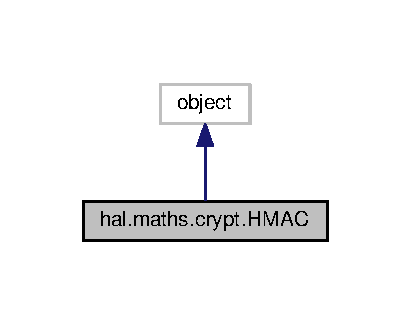
\includegraphics[width=197pt]{classhal_1_1maths_1_1crypt_1_1_h_m_a_c__inherit__graph}
\end{center}
\end{figure}


Collaboration diagram for hal.\+maths.\+crypt.\+H\+M\+AC\+:
\nopagebreak
\begin{figure}[H]
\begin{center}
\leavevmode
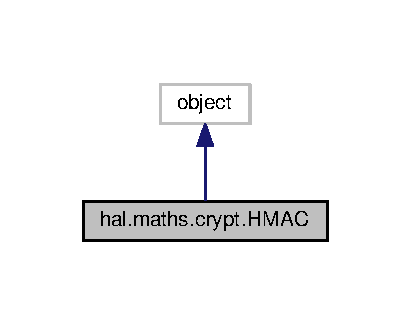
\includegraphics[width=197pt]{classhal_1_1maths_1_1crypt_1_1_h_m_a_c__coll__graph}
\end{center}
\end{figure}
\subsection*{Public Member Functions}
\begin{DoxyCompactItemize}
\item 
def {\bfseries \+\_\+\+\_\+init\+\_\+\+\_\+} (self, string, key)\hypertarget{classhal_1_1maths_1_1crypt_1_1_h_m_a_c_a0186db40c61b717b1ecc0d353272ee14}{}\label{classhal_1_1maths_1_1crypt_1_1_h_m_a_c_a0186db40c61b717b1ecc0d353272ee14}

\item 
def \hyperlink{classhal_1_1maths_1_1crypt_1_1_h_m_a_c_a6c5f1e283f7cb24eddffdda46734e71d}{hash} (self)
\end{DoxyCompactItemize}
\subsection*{Public Attributes}
\begin{DoxyCompactItemize}
\item 
{\bfseries plain}\hypertarget{classhal_1_1maths_1_1crypt_1_1_h_m_a_c_ab910c0e7eb0da6d054812871b920414a}{}\label{classhal_1_1maths_1_1crypt_1_1_h_m_a_c_ab910c0e7eb0da6d054812871b920414a}

\item 
{\bfseries key}\hypertarget{classhal_1_1maths_1_1crypt_1_1_h_m_a_c_a4416aa9252b26f8bf3a401e6d57d44d2}{}\label{classhal_1_1maths_1_1crypt_1_1_h_m_a_c_a4416aa9252b26f8bf3a401e6d57d44d2}

\item 
{\bfseries hashed}\hypertarget{classhal_1_1maths_1_1crypt_1_1_h_m_a_c_aaba6b2465c286591e7c6acf7007c4a32}{}\label{classhal_1_1maths_1_1crypt_1_1_h_m_a_c_aaba6b2465c286591e7c6acf7007c4a32}

\end{DoxyCompactItemize}


\subsection{Detailed Description}
\begin{DoxyVerb}hmac hash \end{DoxyVerb}
 

\subsection{Member Function Documentation}
\index{hal\+::maths\+::crypt\+::\+H\+M\+AC@{hal\+::maths\+::crypt\+::\+H\+M\+AC}!hash@{hash}}
\index{hash@{hash}!hal\+::maths\+::crypt\+::\+H\+M\+AC@{hal\+::maths\+::crypt\+::\+H\+M\+AC}}
\subsubsection[{\texorpdfstring{hash(self)}{hash(self)}}]{\setlength{\rightskip}{0pt plus 5cm}def hal.\+maths.\+crypt.\+H\+M\+A\+C.\+hash (
\begin{DoxyParamCaption}
\item[{}]{self}
\end{DoxyParamCaption}
)}\hypertarget{classhal_1_1maths_1_1crypt_1_1_h_m_a_c_a6c5f1e283f7cb24eddffdda46734e71d}{}\label{classhal_1_1maths_1_1crypt_1_1_h_m_a_c_a6c5f1e283f7cb24eddffdda46734e71d}
\begin{DoxyVerb}:return: hash plaintext
\end{DoxyVerb}
 

The documentation for this class was generated from the following file\+:\begin{DoxyCompactItemize}
\item 
hal/maths/crypt.\+py\end{DoxyCompactItemize}

\hypertarget{classhal_1_1internet_1_1parser_1_1_html_table}{}\section{hal.\+internet.\+parser.\+Html\+Table Class Reference}
\label{classhal_1_1internet_1_1parser_1_1_html_table}\index{hal.\+internet.\+parser.\+Html\+Table@{hal.\+internet.\+parser.\+Html\+Table}}


Inheritance diagram for hal.\+internet.\+parser.\+Html\+Table\+:\nopagebreak
\begin{figure}[H]
\begin{center}
\leavevmode
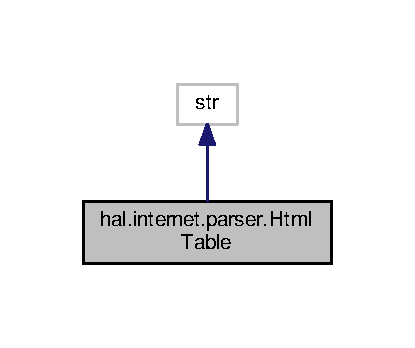
\includegraphics[width=199pt]{classhal_1_1internet_1_1parser_1_1_html_table__inherit__graph}
\end{center}
\end{figure}


Collaboration diagram for hal.\+internet.\+parser.\+Html\+Table\+:\nopagebreak
\begin{figure}[H]
\begin{center}
\leavevmode
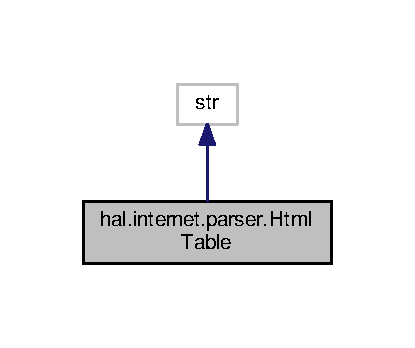
\includegraphics[width=199pt]{classhal_1_1internet_1_1parser_1_1_html_table__coll__graph}
\end{center}
\end{figure}
\subsection*{Public Member Functions}
\begin{DoxyCompactItemize}
\item 
def \hyperlink{classhal_1_1internet_1_1parser_1_1_html_table_a5bcf5b773113fd62eb6b5319372c5e6b}{\+\_\+\+\_\+init\+\_\+\+\_\+} (self, html\+\_\+source)
\item 
def \hyperlink{classhal_1_1internet_1_1parser_1_1_html_table_addcc7238344dce5f6f71426ae03ce362}{parse} (self)
\end{DoxyCompactItemize}
\subsection*{Public Attributes}
\begin{DoxyCompactItemize}
\item 
{\bfseries source}\hypertarget{classhal_1_1internet_1_1parser_1_1_html_table_a537aef3b34a0596a6f7cdf042e6f3089}{}\label{classhal_1_1internet_1_1parser_1_1_html_table_a537aef3b34a0596a6f7cdf042e6f3089}

\item 
{\bfseries soup}\hypertarget{classhal_1_1internet_1_1parser_1_1_html_table_a71408991172cb88eba0ef2ae375746ba}{}\label{classhal_1_1internet_1_1parser_1_1_html_table_a71408991172cb88eba0ef2ae375746ba}

\end{DoxyCompactItemize}


\subsection{Detailed Description}
\begin{DoxyVerb}Table written in HTML language \end{DoxyVerb}
 

\subsection{Constructor \& Destructor Documentation}
\index{hal\+::internet\+::parser\+::\+Html\+Table@{hal\+::internet\+::parser\+::\+Html\+Table}!\+\_\+\+\_\+init\+\_\+\+\_\+@{\+\_\+\+\_\+init\+\_\+\+\_\+}}
\index{\+\_\+\+\_\+init\+\_\+\+\_\+@{\+\_\+\+\_\+init\+\_\+\+\_\+}!hal\+::internet\+::parser\+::\+Html\+Table@{hal\+::internet\+::parser\+::\+Html\+Table}}
\subsubsection[{\texorpdfstring{\+\_\+\+\_\+init\+\_\+\+\_\+(self, html\+\_\+source)}{__init__(self, html_source)}}]{\setlength{\rightskip}{0pt plus 5cm}def hal.\+internet.\+parser.\+Html\+Table.\+\_\+\+\_\+init\+\_\+\+\_\+ (
\begin{DoxyParamCaption}
\item[{}]{self, }
\item[{}]{html\+\_\+source}
\end{DoxyParamCaption}
)}\hypertarget{classhal_1_1internet_1_1parser_1_1_html_table_a5bcf5b773113fd62eb6b5319372c5e6b}{}\label{classhal_1_1internet_1_1parser_1_1_html_table_a5bcf5b773113fd62eb6b5319372c5e6b}
\begin{DoxyVerb}:param html_source: string
    Html source of table
\end{DoxyVerb}
 

\subsection{Member Function Documentation}
\index{hal\+::internet\+::parser\+::\+Html\+Table@{hal\+::internet\+::parser\+::\+Html\+Table}!parse@{parse}}
\index{parse@{parse}!hal\+::internet\+::parser\+::\+Html\+Table@{hal\+::internet\+::parser\+::\+Html\+Table}}
\subsubsection[{\texorpdfstring{parse(self)}{parse(self)}}]{\setlength{\rightskip}{0pt plus 5cm}def hal.\+internet.\+parser.\+Html\+Table.\+parse (
\begin{DoxyParamCaption}
\item[{}]{self}
\end{DoxyParamCaption}
)}\hypertarget{classhal_1_1internet_1_1parser_1_1_html_table_addcc7238344dce5f6f71426ae03ce362}{}\label{classhal_1_1internet_1_1parser_1_1_html_table_addcc7238344dce5f6f71426ae03ce362}
\begin{DoxyVerb}:return: list of list
    List of list of values in table
\end{DoxyVerb}
 

The documentation for this class was generated from the following file\+:\begin{DoxyCompactItemize}
\item 
/home/stefano/\+Coding/\+Python/projects/pyhal/hal/internet/parser.\+py\end{DoxyCompactItemize}

\hypertarget{classhal_1_1maths_1_1crypt_1_1_i_d_e_a}{}\section{hal.\+maths.\+crypt.\+I\+D\+EA Class Reference}
\label{classhal_1_1maths_1_1crypt_1_1_i_d_e_a}\index{hal.\+maths.\+crypt.\+I\+D\+EA@{hal.\+maths.\+crypt.\+I\+D\+EA}}


Inheritance diagram for hal.\+maths.\+crypt.\+I\+D\+EA\+:
\nopagebreak
\begin{figure}[H]
\begin{center}
\leavevmode
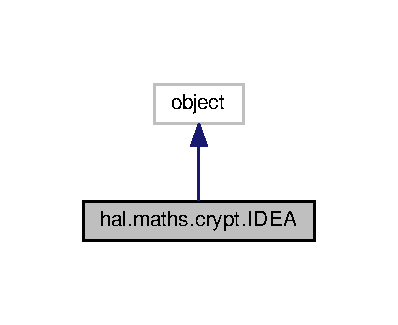
\includegraphics[width=191pt]{classhal_1_1maths_1_1crypt_1_1_i_d_e_a__inherit__graph}
\end{center}
\end{figure}


Collaboration diagram for hal.\+maths.\+crypt.\+I\+D\+EA\+:
\nopagebreak
\begin{figure}[H]
\begin{center}
\leavevmode
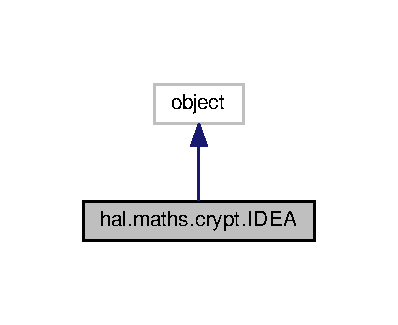
\includegraphics[width=191pt]{classhal_1_1maths_1_1crypt_1_1_i_d_e_a__coll__graph}
\end{center}
\end{figure}
\subsection*{Public Member Functions}
\begin{DoxyCompactItemize}
\item 
def {\bfseries \+\_\+\+\_\+init\+\_\+\+\_\+} (self, string, key)\hypertarget{classhal_1_1maths_1_1crypt_1_1_i_d_e_a_aeef99d9276abb6b2bd57d001c909dce6}{}\label{classhal_1_1maths_1_1crypt_1_1_i_d_e_a_aeef99d9276abb6b2bd57d001c909dce6}

\item 
def \hyperlink{classhal_1_1maths_1_1crypt_1_1_i_d_e_a_a35ca1846d9e5373e9c8ded2515926a75}{hash} (self)
\item 
def \hyperlink{classhal_1_1maths_1_1crypt_1_1_i_d_e_a_affd2617aac36358891d86f2cb1fc39c4}{change\+\_\+key} (self, key)
\item 
def \hyperlink{classhal_1_1maths_1_1crypt_1_1_i_d_e_a_a8950639a4067643433ae9db631d3c8d0}{encrypt} (self)
\end{DoxyCompactItemize}
\subsection*{Public Attributes}
\begin{DoxyCompactItemize}
\item 
{\bfseries plain}\hypertarget{classhal_1_1maths_1_1crypt_1_1_i_d_e_a_a3e7cfa1f3b0c243b2b7804b3c08e84bd}{}\label{classhal_1_1maths_1_1crypt_1_1_i_d_e_a_a3e7cfa1f3b0c243b2b7804b3c08e84bd}

\item 
{\bfseries hashed}\hypertarget{classhal_1_1maths_1_1crypt_1_1_i_d_e_a_a0c8e325b0c159234ac90d9e32006fbc8}{}\label{classhal_1_1maths_1_1crypt_1_1_i_d_e_a_a0c8e325b0c159234ac90d9e32006fbc8}

\end{DoxyCompactItemize}


\subsection{Detailed Description}
\begin{DoxyVerb}IDEA hash \end{DoxyVerb}
 

\subsection{Member Function Documentation}
\index{hal\+::maths\+::crypt\+::\+I\+D\+EA@{hal\+::maths\+::crypt\+::\+I\+D\+EA}!change\+\_\+key@{change\+\_\+key}}
\index{change\+\_\+key@{change\+\_\+key}!hal\+::maths\+::crypt\+::\+I\+D\+EA@{hal\+::maths\+::crypt\+::\+I\+D\+EA}}
\subsubsection[{\texorpdfstring{change\+\_\+key(self, key)}{change_key(self, key)}}]{\setlength{\rightskip}{0pt plus 5cm}def hal.\+maths.\+crypt.\+I\+D\+E\+A.\+change\+\_\+key (
\begin{DoxyParamCaption}
\item[{}]{self, }
\item[{}]{key}
\end{DoxyParamCaption}
)}\hypertarget{classhal_1_1maths_1_1crypt_1_1_i_d_e_a_affd2617aac36358891d86f2cb1fc39c4}{}\label{classhal_1_1maths_1_1crypt_1_1_i_d_e_a_affd2617aac36358891d86f2cb1fc39c4}
\begin{DoxyVerb}:param key: new key
:return: change key
\end{DoxyVerb}
 \index{hal\+::maths\+::crypt\+::\+I\+D\+EA@{hal\+::maths\+::crypt\+::\+I\+D\+EA}!encrypt@{encrypt}}
\index{encrypt@{encrypt}!hal\+::maths\+::crypt\+::\+I\+D\+EA@{hal\+::maths\+::crypt\+::\+I\+D\+EA}}
\subsubsection[{\texorpdfstring{encrypt(self)}{encrypt(self)}}]{\setlength{\rightskip}{0pt plus 5cm}def hal.\+maths.\+crypt.\+I\+D\+E\+A.\+encrypt (
\begin{DoxyParamCaption}
\item[{}]{self}
\end{DoxyParamCaption}
)}\hypertarget{classhal_1_1maths_1_1crypt_1_1_i_d_e_a_a8950639a4067643433ae9db631d3c8d0}{}\label{classhal_1_1maths_1_1crypt_1_1_i_d_e_a_a8950639a4067643433ae9db631d3c8d0}
\begin{DoxyVerb}:return: encrypt with key
\end{DoxyVerb}
 \index{hal\+::maths\+::crypt\+::\+I\+D\+EA@{hal\+::maths\+::crypt\+::\+I\+D\+EA}!hash@{hash}}
\index{hash@{hash}!hal\+::maths\+::crypt\+::\+I\+D\+EA@{hal\+::maths\+::crypt\+::\+I\+D\+EA}}
\subsubsection[{\texorpdfstring{hash(self)}{hash(self)}}]{\setlength{\rightskip}{0pt plus 5cm}def hal.\+maths.\+crypt.\+I\+D\+E\+A.\+hash (
\begin{DoxyParamCaption}
\item[{}]{self}
\end{DoxyParamCaption}
)}\hypertarget{classhal_1_1maths_1_1crypt_1_1_i_d_e_a_a35ca1846d9e5373e9c8ded2515926a75}{}\label{classhal_1_1maths_1_1crypt_1_1_i_d_e_a_a35ca1846d9e5373e9c8ded2515926a75}
\begin{DoxyVerb}:return: IDEA hash
\end{DoxyVerb}
 

The documentation for this class was generated from the following file\+:\begin{DoxyCompactItemize}
\item 
hal/maths/crypt.\+py\end{DoxyCompactItemize}

\hypertarget{classhal_1_1maths_1_1maths_1_1_integer}{}\section{hal.\+maths.\+maths.\+Integer Class Reference}
\label{classhal_1_1maths_1_1maths_1_1_integer}\index{hal.\+maths.\+maths.\+Integer@{hal.\+maths.\+maths.\+Integer}}


Inheritance diagram for hal.\+maths.\+maths.\+Integer\+:\nopagebreak
\begin{figure}[H]
\begin{center}
\leavevmode
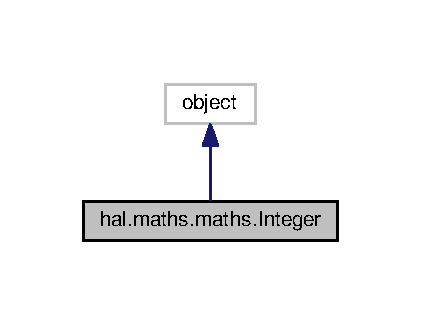
\includegraphics[width=202pt]{classhal_1_1maths_1_1maths_1_1_integer__inherit__graph}
\end{center}
\end{figure}


Collaboration diagram for hal.\+maths.\+maths.\+Integer\+:\nopagebreak
\begin{figure}[H]
\begin{center}
\leavevmode
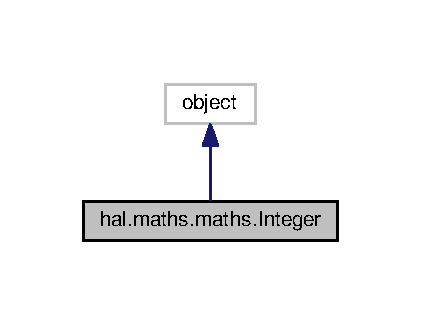
\includegraphics[width=202pt]{classhal_1_1maths_1_1maths_1_1_integer__coll__graph}
\end{center}
\end{figure}
\subsection*{Public Member Functions}
\begin{DoxyCompactItemize}
\item 
def {\bfseries \+\_\+\+\_\+init\+\_\+\+\_\+} (self, string)\hypertarget{classhal_1_1maths_1_1maths_1_1_integer_ab02daf8f7df66b9739514805740d2e29}{}\label{classhal_1_1maths_1_1maths_1_1_integer_ab02daf8f7df66b9739514805740d2e29}

\item 
def \hyperlink{classhal_1_1maths_1_1maths_1_1_integer_a5833e790dc98122d0e5d0e92fb5bee49}{is\+\_\+naive\+\_\+prime} (self)
\item 
def \hyperlink{classhal_1_1maths_1_1maths_1_1_integer_a813e392f81a6c01f87a9ef8d1c8c1250}{is\+\_\+probably\+\_\+prime} (self)
\item 
def \hyperlink{classhal_1_1maths_1_1maths_1_1_integer_a3cd7d69cc1e8bb8271e61bbeba6d2a50}{test\+\_\+miller\+\_\+rabin} (self, precision)
\end{DoxyCompactItemize}
\subsection*{Public Attributes}
\begin{DoxyCompactItemize}
\item 
{\bfseries to\+\_\+int}\hypertarget{classhal_1_1maths_1_1maths_1_1_integer_aef52e227e80e9dc90779d0d8f202dbc6}{}\label{classhal_1_1maths_1_1maths_1_1_integer_aef52e227e80e9dc90779d0d8f202dbc6}

\item 
{\bfseries to\+\_\+string}\hypertarget{classhal_1_1maths_1_1maths_1_1_integer_a18958bf743811b233e9524cbaf355138}{}\label{classhal_1_1maths_1_1maths_1_1_integer_a18958bf743811b233e9524cbaf355138}

\end{DoxyCompactItemize}


\subsection{Detailed Description}
\begin{DoxyVerb}Big int std python won't recognize \end{DoxyVerb}
 

\subsection{Member Function Documentation}
\index{hal\+::maths\+::maths\+::\+Integer@{hal\+::maths\+::maths\+::\+Integer}!is\+\_\+naive\+\_\+prime@{is\+\_\+naive\+\_\+prime}}
\index{is\+\_\+naive\+\_\+prime@{is\+\_\+naive\+\_\+prime}!hal\+::maths\+::maths\+::\+Integer@{hal\+::maths\+::maths\+::\+Integer}}
\subsubsection[{\texorpdfstring{is\+\_\+naive\+\_\+prime(self)}{is_naive_prime(self)}}]{\setlength{\rightskip}{0pt plus 5cm}def hal.\+maths.\+maths.\+Integer.\+is\+\_\+naive\+\_\+prime (
\begin{DoxyParamCaption}
\item[{}]{self}
\end{DoxyParamCaption}
)}\hypertarget{classhal_1_1maths_1_1maths_1_1_integer_a5833e790dc98122d0e5d0e92fb5bee49}{}\label{classhal_1_1maths_1_1maths_1_1_integer_a5833e790dc98122d0e5d0e92fb5bee49}
\begin{DoxyVerb}:return: bool
    Checks if prime in very naive way
\end{DoxyVerb}
 \index{hal\+::maths\+::maths\+::\+Integer@{hal\+::maths\+::maths\+::\+Integer}!is\+\_\+probably\+\_\+prime@{is\+\_\+probably\+\_\+prime}}
\index{is\+\_\+probably\+\_\+prime@{is\+\_\+probably\+\_\+prime}!hal\+::maths\+::maths\+::\+Integer@{hal\+::maths\+::maths\+::\+Integer}}
\subsubsection[{\texorpdfstring{is\+\_\+probably\+\_\+prime(self)}{is_probably_prime(self)}}]{\setlength{\rightskip}{0pt plus 5cm}def hal.\+maths.\+maths.\+Integer.\+is\+\_\+probably\+\_\+prime (
\begin{DoxyParamCaption}
\item[{}]{self}
\end{DoxyParamCaption}
)}\hypertarget{classhal_1_1maths_1_1maths_1_1_integer_a813e392f81a6c01f87a9ef8d1c8c1250}{}\label{classhal_1_1maths_1_1maths_1_1_integer_a813e392f81a6c01f87a9ef8d1c8c1250}
\begin{DoxyVerb}:return: test with miller-rabin
\end{DoxyVerb}
 \index{hal\+::maths\+::maths\+::\+Integer@{hal\+::maths\+::maths\+::\+Integer}!test\+\_\+miller\+\_\+rabin@{test\+\_\+miller\+\_\+rabin}}
\index{test\+\_\+miller\+\_\+rabin@{test\+\_\+miller\+\_\+rabin}!hal\+::maths\+::maths\+::\+Integer@{hal\+::maths\+::maths\+::\+Integer}}
\subsubsection[{\texorpdfstring{test\+\_\+miller\+\_\+rabin(self, precision)}{test_miller_rabin(self, precision)}}]{\setlength{\rightskip}{0pt plus 5cm}def hal.\+maths.\+maths.\+Integer.\+test\+\_\+miller\+\_\+rabin (
\begin{DoxyParamCaption}
\item[{}]{self, }
\item[{}]{precision}
\end{DoxyParamCaption}
)}\hypertarget{classhal_1_1maths_1_1maths_1_1_integer_a3cd7d69cc1e8bb8271e61bbeba6d2a50}{}\label{classhal_1_1maths_1_1maths_1_1_integer_a3cd7d69cc1e8bb8271e61bbeba6d2a50}
\begin{DoxyVerb}:param precision: number of rounds to perform (higher -> better
precision)
:return: True iff probably prime
\end{DoxyVerb}
 

The documentation for this class was generated from the following file\+:\begin{DoxyCompactItemize}
\item 
/home/stefano/\+Coding/\+Python/projects/pyhal/hal/maths/maths.\+py\end{DoxyCompactItemize}

\hypertarget{classhal_1_1maths_1_1crypt_1_1_m_d5}{}\section{hal.\+maths.\+crypt.\+M\+D5 Class Reference}
\label{classhal_1_1maths_1_1crypt_1_1_m_d5}\index{hal.\+maths.\+crypt.\+M\+D5@{hal.\+maths.\+crypt.\+M\+D5}}


Inheritance diagram for hal.\+maths.\+crypt.\+M\+D5\+:
\nopagebreak
\begin{figure}[H]
\begin{center}
\leavevmode
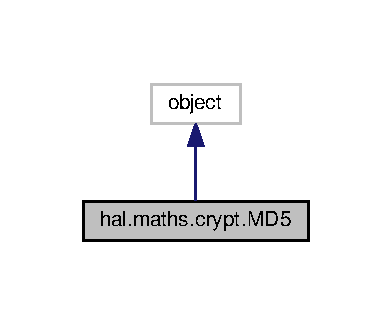
\includegraphics[width=188pt]{classhal_1_1maths_1_1crypt_1_1_m_d5__inherit__graph}
\end{center}
\end{figure}


Collaboration diagram for hal.\+maths.\+crypt.\+M\+D5\+:
\nopagebreak
\begin{figure}[H]
\begin{center}
\leavevmode
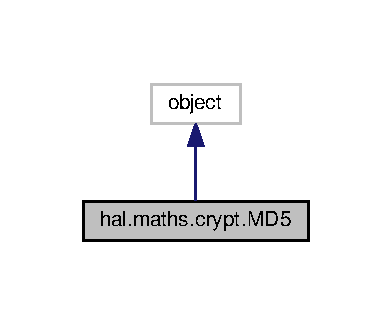
\includegraphics[width=188pt]{classhal_1_1maths_1_1crypt_1_1_m_d5__coll__graph}
\end{center}
\end{figure}
\subsection*{Public Member Functions}
\begin{DoxyCompactItemize}
\item 
def {\bfseries \+\_\+\+\_\+init\+\_\+\+\_\+} (self, string)\hypertarget{classhal_1_1maths_1_1crypt_1_1_m_d5_a904093421d68e73ab12f6d00f3e0beff}{}\label{classhal_1_1maths_1_1crypt_1_1_m_d5_a904093421d68e73ab12f6d00f3e0beff}

\item 
def \hyperlink{classhal_1_1maths_1_1crypt_1_1_m_d5_a5f2fcd9c5019f5ace7f70f7a6b514123}{hash} (self)
\end{DoxyCompactItemize}
\subsection*{Public Attributes}
\begin{DoxyCompactItemize}
\item 
{\bfseries plain}\hypertarget{classhal_1_1maths_1_1crypt_1_1_m_d5_aa822e9fbe6057d9aa720551bdba468e6}{}\label{classhal_1_1maths_1_1crypt_1_1_m_d5_aa822e9fbe6057d9aa720551bdba468e6}

\item 
{\bfseries hashed}\hypertarget{classhal_1_1maths_1_1crypt_1_1_m_d5_a7f9b85649d89714b340a6dfb424681a2}{}\label{classhal_1_1maths_1_1crypt_1_1_m_d5_a7f9b85649d89714b340a6dfb424681a2}

\end{DoxyCompactItemize}


\subsection{Detailed Description}
\begin{DoxyVerb}md5 hash \end{DoxyVerb}
 

\subsection{Member Function Documentation}
\index{hal\+::maths\+::crypt\+::\+M\+D5@{hal\+::maths\+::crypt\+::\+M\+D5}!hash@{hash}}
\index{hash@{hash}!hal\+::maths\+::crypt\+::\+M\+D5@{hal\+::maths\+::crypt\+::\+M\+D5}}
\subsubsection[{\texorpdfstring{hash(self)}{hash(self)}}]{\setlength{\rightskip}{0pt plus 5cm}def hal.\+maths.\+crypt.\+M\+D5.\+hash (
\begin{DoxyParamCaption}
\item[{}]{self}
\end{DoxyParamCaption}
)}\hypertarget{classhal_1_1maths_1_1crypt_1_1_m_d5_a5f2fcd9c5019f5ace7f70f7a6b514123}{}\label{classhal_1_1maths_1_1crypt_1_1_m_d5_a5f2fcd9c5019f5ace7f70f7a6b514123}
\begin{DoxyVerb}:return: hash plaintext
\end{DoxyVerb}
 

The documentation for this class was generated from the following file\+:\begin{DoxyCompactItemize}
\item 
hal/maths/crypt.\+py\end{DoxyCompactItemize}

\hypertarget{classhal_1_1maths_1_1crypt_1_1_m_d6}{}\section{hal.\+maths.\+crypt.\+M\+D6 Class Reference}
\label{classhal_1_1maths_1_1crypt_1_1_m_d6}\index{hal.\+maths.\+crypt.\+M\+D6@{hal.\+maths.\+crypt.\+M\+D6}}


Inheritance diagram for hal.\+maths.\+crypt.\+M\+D6\+:
\nopagebreak
\begin{figure}[H]
\begin{center}
\leavevmode
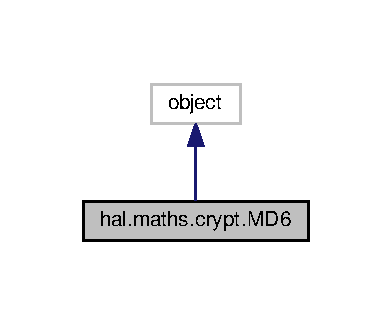
\includegraphics[width=188pt]{classhal_1_1maths_1_1crypt_1_1_m_d6__inherit__graph}
\end{center}
\end{figure}


Collaboration diagram for hal.\+maths.\+crypt.\+M\+D6\+:
\nopagebreak
\begin{figure}[H]
\begin{center}
\leavevmode
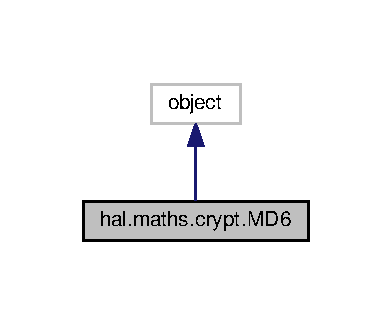
\includegraphics[width=188pt]{classhal_1_1maths_1_1crypt_1_1_m_d6__coll__graph}
\end{center}
\end{figure}
\subsection*{Public Member Functions}
\begin{DoxyCompactItemize}
\item 
def {\bfseries \+\_\+\+\_\+init\+\_\+\+\_\+} (self, string, size)\hypertarget{classhal_1_1maths_1_1crypt_1_1_m_d6_a44aaff6ac5a1369c30c6515e36f3e4f2}{}\label{classhal_1_1maths_1_1crypt_1_1_m_d6_a44aaff6ac5a1369c30c6515e36f3e4f2}

\item 
def \hyperlink{classhal_1_1maths_1_1crypt_1_1_m_d6_ad3e597a2acb6d2e2ff3dbccdde536ab1}{hash} (self)
\item 
def \hyperlink{classhal_1_1maths_1_1crypt_1_1_m_d6_abe7af5abf04e41a31b3c901124aa1114}{hex} (self, data, size)
\item 
def \hyperlink{classhal_1_1maths_1_1crypt_1_1_m_d6_a325f687cdf1081ae62d54638a5774293}{raw} (self, data, size)
\end{DoxyCompactItemize}
\subsection*{Public Attributes}
\begin{DoxyCompactItemize}
\item 
{\bfseries plain}\hypertarget{classhal_1_1maths_1_1crypt_1_1_m_d6_a278814da97344037e49882218a3e5f99}{}\label{classhal_1_1maths_1_1crypt_1_1_m_d6_a278814da97344037e49882218a3e5f99}

\item 
{\bfseries size}\hypertarget{classhal_1_1maths_1_1crypt_1_1_m_d6_ac536bb3b4e1a4099845865e51e31291f}{}\label{classhal_1_1maths_1_1crypt_1_1_m_d6_ac536bb3b4e1a4099845865e51e31291f}

\item 
{\bfseries hashed}\hypertarget{classhal_1_1maths_1_1crypt_1_1_m_d6_a4f2445ec801202f1eefed4c428778ea8}{}\label{classhal_1_1maths_1_1crypt_1_1_m_d6_a4f2445ec801202f1eefed4c428778ea8}

\end{DoxyCompactItemize}
\subsection*{Static Public Attributes}
\begin{DoxyCompactItemize}
\item 
list {\bfseries A\+L\+L\+O\+W\+E\+D\+\_\+\+S\+I\+ZE} = \mbox{[}64, 128, 224, 256, 384, 512\mbox{]}\hypertarget{classhal_1_1maths_1_1crypt_1_1_m_d6_a54b930b58adc82ff6fb00b7ec03b9194}{}\label{classhal_1_1maths_1_1crypt_1_1_m_d6_a54b930b58adc82ff6fb00b7ec03b9194}

\end{DoxyCompactItemize}


\subsection{Detailed Description}
\begin{DoxyVerb}md6 hash \end{DoxyVerb}
 

\subsection{Member Function Documentation}
\index{hal\+::maths\+::crypt\+::\+M\+D6@{hal\+::maths\+::crypt\+::\+M\+D6}!hash@{hash}}
\index{hash@{hash}!hal\+::maths\+::crypt\+::\+M\+D6@{hal\+::maths\+::crypt\+::\+M\+D6}}
\subsubsection[{\texorpdfstring{hash(self)}{hash(self)}}]{\setlength{\rightskip}{0pt plus 5cm}def hal.\+maths.\+crypt.\+M\+D6.\+hash (
\begin{DoxyParamCaption}
\item[{}]{self}
\end{DoxyParamCaption}
)}\hypertarget{classhal_1_1maths_1_1crypt_1_1_m_d6_ad3e597a2acb6d2e2ff3dbccdde536ab1}{}\label{classhal_1_1maths_1_1crypt_1_1_m_d6_ad3e597a2acb6d2e2ff3dbccdde536ab1}
\begin{DoxyVerb}:return: return md6 hash
\end{DoxyVerb}
 \index{hal\+::maths\+::crypt\+::\+M\+D6@{hal\+::maths\+::crypt\+::\+M\+D6}!hex@{hex}}
\index{hex@{hex}!hal\+::maths\+::crypt\+::\+M\+D6@{hal\+::maths\+::crypt\+::\+M\+D6}}
\subsubsection[{\texorpdfstring{hex(self, data, size)}{hex(self, data, size)}}]{\setlength{\rightskip}{0pt plus 5cm}def hal.\+maths.\+crypt.\+M\+D6.\+hex (
\begin{DoxyParamCaption}
\item[{}]{self, }
\item[{}]{data, }
\item[{}]{size}
\end{DoxyParamCaption}
)}\hypertarget{classhal_1_1maths_1_1crypt_1_1_m_d6_abe7af5abf04e41a31b3c901124aa1114}{}\label{classhal_1_1maths_1_1crypt_1_1_m_d6_abe7af5abf04e41a31b3c901124aa1114}
\begin{DoxyVerb}:param data: plaintext
:param size: bytes
:return: hex representation
\end{DoxyVerb}
 \index{hal\+::maths\+::crypt\+::\+M\+D6@{hal\+::maths\+::crypt\+::\+M\+D6}!raw@{raw}}
\index{raw@{raw}!hal\+::maths\+::crypt\+::\+M\+D6@{hal\+::maths\+::crypt\+::\+M\+D6}}
\subsubsection[{\texorpdfstring{raw(self, data, size)}{raw(self, data, size)}}]{\setlength{\rightskip}{0pt plus 5cm}def hal.\+maths.\+crypt.\+M\+D6.\+raw (
\begin{DoxyParamCaption}
\item[{}]{self, }
\item[{}]{data, }
\item[{}]{size}
\end{DoxyParamCaption}
)}\hypertarget{classhal_1_1maths_1_1crypt_1_1_m_d6_a325f687cdf1081ae62d54638a5774293}{}\label{classhal_1_1maths_1_1crypt_1_1_m_d6_a325f687cdf1081ae62d54638a5774293}
\begin{DoxyVerb}:param data: plaintext
:param size: bytes
:return: raw representation
\end{DoxyVerb}
 

The documentation for this class was generated from the following file\+:\begin{DoxyCompactItemize}
\item 
hal/maths/crypt.\+py\end{DoxyCompactItemize}

\hypertarget{classhal_1_1files_1_1models_1_1_m_p3_song}{}\section{hal.\+files.\+models.\+M\+P3\+Song Class Reference}
\label{classhal_1_1files_1_1models_1_1_m_p3_song}\index{hal.\+files.\+models.\+M\+P3\+Song@{hal.\+files.\+models.\+M\+P3\+Song}}


Inheritance diagram for hal.\+files.\+models.\+M\+P3\+Song\+:\nopagebreak
\begin{figure}[H]
\begin{center}
\leavevmode
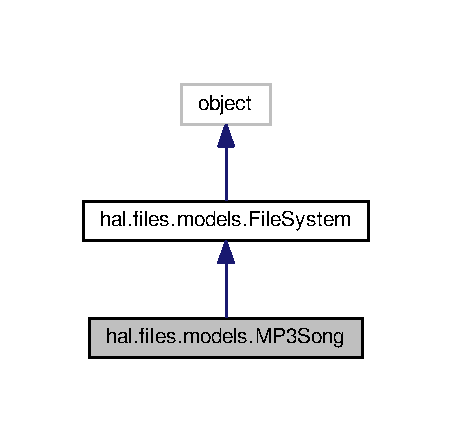
\includegraphics[width=217pt]{classhal_1_1files_1_1models_1_1_m_p3_song__inherit__graph}
\end{center}
\end{figure}


Collaboration diagram for hal.\+files.\+models.\+M\+P3\+Song\+:\nopagebreak
\begin{figure}[H]
\begin{center}
\leavevmode
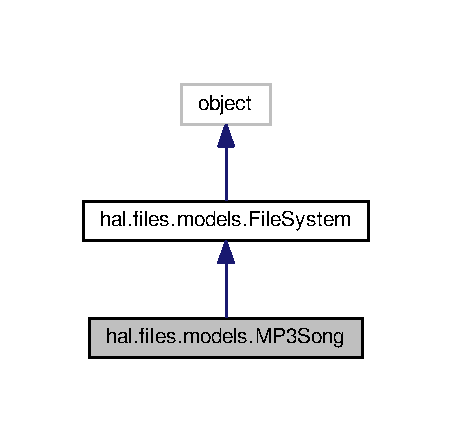
\includegraphics[width=217pt]{classhal_1_1files_1_1models_1_1_m_p3_song__coll__graph}
\end{center}
\end{figure}
\subsection*{Public Member Functions}
\begin{DoxyCompactItemize}
\item 
def {\bfseries \+\_\+\+\_\+init\+\_\+\+\_\+} (self, path)\hypertarget{classhal_1_1files_1_1models_1_1_m_p3_song_a4f37efc2f666bf142bb1ed2370244fef}{}\label{classhal_1_1files_1_1models_1_1_m_p3_song_a4f37efc2f666bf142bb1ed2370244fef}

\item 
def {\bfseries set\+\_\+name} (self, name)\hypertarget{classhal_1_1files_1_1models_1_1_m_p3_song_ae4f958b7afa7212cff8470163854a0ed}{}\label{classhal_1_1files_1_1models_1_1_m_p3_song_ae4f958b7afa7212cff8470163854a0ed}

\item 
def {\bfseries set\+\_\+artist} (self, artist)\hypertarget{classhal_1_1files_1_1models_1_1_m_p3_song_abecb2c34045dbd2133e898114198d518}{}\label{classhal_1_1files_1_1models_1_1_m_p3_song_abecb2c34045dbd2133e898114198d518}

\item 
def {\bfseries set\+\_\+album} (self, album)\hypertarget{classhal_1_1files_1_1models_1_1_m_p3_song_afda62b2b1519b7bc65e8cd98d8f2e2bf}{}\label{classhal_1_1files_1_1models_1_1_m_p3_song_afda62b2b1519b7bc65e8cd98d8f2e2bf}

\item 
def {\bfseries set\+\_\+nr\+\_\+track} (self, nr\+\_\+track)\hypertarget{classhal_1_1files_1_1models_1_1_m_p3_song_a6b456dde38763b13fb10266b7910b63f}{}\label{classhal_1_1files_1_1models_1_1_m_p3_song_a6b456dde38763b13fb10266b7910b63f}

\item 
def {\bfseries set\+\_\+year} (self, year)\hypertarget{classhal_1_1files_1_1models_1_1_m_p3_song_ac14c40460b53a47979a58864409a366c}{}\label{classhal_1_1files_1_1models_1_1_m_p3_song_ac14c40460b53a47979a58864409a366c}

\end{DoxyCompactItemize}
\subsection*{Public Attributes}
\begin{DoxyCompactItemize}
\item 
{\bfseries song}\hypertarget{classhal_1_1files_1_1models_1_1_m_p3_song_a767b9af9e2e01ce942a44cfa7cda2653}{}\label{classhal_1_1files_1_1models_1_1_m_p3_song_a767b9af9e2e01ce942a44cfa7cda2653}

\item 
{\bfseries tags}\hypertarget{classhal_1_1files_1_1models_1_1_m_p3_song_a57a2d42a3326e55f553c1a79678dd6b5}{}\label{classhal_1_1files_1_1models_1_1_m_p3_song_a57a2d42a3326e55f553c1a79678dd6b5}

\end{DoxyCompactItemize}
\subsection*{Additional Inherited Members}


\subsection{Detailed Description}
\begin{DoxyVerb}mp3 song \end{DoxyVerb}
 

The documentation for this class was generated from the following file\+:\begin{DoxyCompactItemize}
\item 
/home/stefano/\+Coding/\+Python/projects/pyhal/hal/files/models.\+py\end{DoxyCompactItemize}

\hypertarget{classhal_1_1ml_1_1data_1_1parser_1_1_parser}{}\section{hal.\+ml.\+data.\+parser.\+Parser Class Reference}
\label{classhal_1_1ml_1_1data_1_1parser_1_1_parser}\index{hal.\+ml.\+data.\+parser.\+Parser@{hal.\+ml.\+data.\+parser.\+Parser}}


Inheritance diagram for hal.\+ml.\+data.\+parser.\+Parser\+:\nopagebreak
\begin{figure}[H]
\begin{center}
\leavevmode
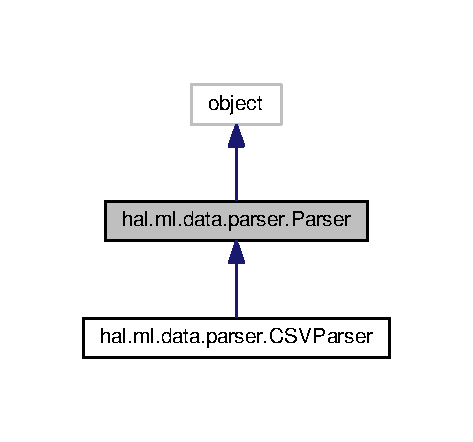
\includegraphics[width=227pt]{classhal_1_1ml_1_1data_1_1parser_1_1_parser__inherit__graph}
\end{center}
\end{figure}


Collaboration diagram for hal.\+ml.\+data.\+parser.\+Parser\+:\nopagebreak
\begin{figure}[H]
\begin{center}
\leavevmode
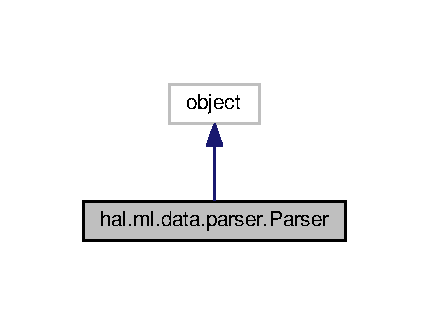
\includegraphics[width=206pt]{classhal_1_1ml_1_1data_1_1parser_1_1_parser__coll__graph}
\end{center}
\end{figure}
\subsection*{Public Member Functions}
\begin{DoxyCompactItemize}
\item 
def \hyperlink{classhal_1_1ml_1_1data_1_1parser_1_1_parser_adc7a4812823d9c636eb8977c6d450e6a}{\+\_\+\+\_\+init\+\_\+\+\_\+} (self, database\+\_\+file)
\item 
def \hyperlink{classhal_1_1ml_1_1data_1_1parser_1_1_parser_aaf10b0c434100a1c3effd5e5ee0ee2a3}{get\+\_\+lines} (self)
\end{DoxyCompactItemize}
\subsection*{Public Attributes}
\begin{DoxyCompactItemize}
\item 
{\bfseries database\+\_\+file}\hypertarget{classhal_1_1ml_1_1data_1_1parser_1_1_parser_a6c29e08c2a9938a625004389ef18a281}{}\label{classhal_1_1ml_1_1data_1_1parser_1_1_parser_a6c29e08c2a9938a625004389ef18a281}

\item 
{\bfseries lines}\hypertarget{classhal_1_1ml_1_1data_1_1parser_1_1_parser_a7409c542f418415aeb0c073be705fc58}{}\label{classhal_1_1ml_1_1data_1_1parser_1_1_parser_a7409c542f418415aeb0c073be705fc58}

\end{DoxyCompactItemize}


\subsection{Detailed Description}
\begin{DoxyVerb}Mother of all data-files parsers \end{DoxyVerb}
 

\subsection{Constructor \& Destructor Documentation}
\index{hal\+::ml\+::data\+::parser\+::\+Parser@{hal\+::ml\+::data\+::parser\+::\+Parser}!\+\_\+\+\_\+init\+\_\+\+\_\+@{\+\_\+\+\_\+init\+\_\+\+\_\+}}
\index{\+\_\+\+\_\+init\+\_\+\+\_\+@{\+\_\+\+\_\+init\+\_\+\+\_\+}!hal\+::ml\+::data\+::parser\+::\+Parser@{hal\+::ml\+::data\+::parser\+::\+Parser}}
\subsubsection[{\texorpdfstring{\+\_\+\+\_\+init\+\_\+\+\_\+(self, database\+\_\+file)}{__init__(self, database_file)}}]{\setlength{\rightskip}{0pt plus 5cm}def hal.\+ml.\+data.\+parser.\+Parser.\+\_\+\+\_\+init\+\_\+\+\_\+ (
\begin{DoxyParamCaption}
\item[{}]{self, }
\item[{}]{database\+\_\+file}
\end{DoxyParamCaption}
)}\hypertarget{classhal_1_1ml_1_1data_1_1parser_1_1_parser_adc7a4812823d9c636eb8977c6d450e6a}{}\label{classhal_1_1ml_1_1data_1_1parser_1_1_parser_adc7a4812823d9c636eb8977c6d450e6a}
\begin{DoxyVerb}:param database_file: a raw .csv file that contains any data
about anything \end{DoxyVerb}
 

\subsection{Member Function Documentation}
\index{hal\+::ml\+::data\+::parser\+::\+Parser@{hal\+::ml\+::data\+::parser\+::\+Parser}!get\+\_\+lines@{get\+\_\+lines}}
\index{get\+\_\+lines@{get\+\_\+lines}!hal\+::ml\+::data\+::parser\+::\+Parser@{hal\+::ml\+::data\+::parser\+::\+Parser}}
\subsubsection[{\texorpdfstring{get\+\_\+lines(self)}{get_lines(self)}}]{\setlength{\rightskip}{0pt plus 5cm}def hal.\+ml.\+data.\+parser.\+Parser.\+get\+\_\+lines (
\begin{DoxyParamCaption}
\item[{}]{self}
\end{DoxyParamCaption}
)}\hypertarget{classhal_1_1ml_1_1data_1_1parser_1_1_parser_aaf10b0c434100a1c3effd5e5ee0ee2a3}{}\label{classhal_1_1ml_1_1data_1_1parser_1_1_parser_aaf10b0c434100a1c3effd5e5ee0ee2a3}
\begin{DoxyVerb}:return: [] of str
    Lines in file
\end{DoxyVerb}
 

The documentation for this class was generated from the following file\+:\begin{DoxyCompactItemize}
\item 
/home/stefano/\+Coding/\+Python/projects/pyhal/hal/ml/data/parser.\+py\end{DoxyCompactItemize}

\hypertarget{classhal_1_1maths_1_1plotter_1_1_plot2d}{}\section{hal.\+maths.\+plotter.\+Plot2d Class Reference}
\label{classhal_1_1maths_1_1plotter_1_1_plot2d}\index{hal.\+maths.\+plotter.\+Plot2d@{hal.\+maths.\+plotter.\+Plot2d}}


Inheritance diagram for hal.\+maths.\+plotter.\+Plot2d\+:
\nopagebreak
\begin{figure}[H]
\begin{center}
\leavevmode
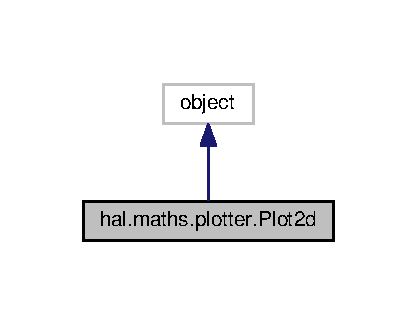
\includegraphics[width=200pt]{classhal_1_1maths_1_1plotter_1_1_plot2d__inherit__graph}
\end{center}
\end{figure}


Collaboration diagram for hal.\+maths.\+plotter.\+Plot2d\+:
\nopagebreak
\begin{figure}[H]
\begin{center}
\leavevmode
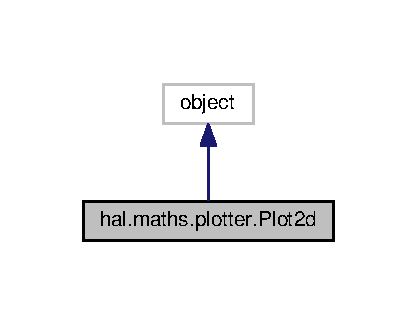
\includegraphics[width=200pt]{classhal_1_1maths_1_1plotter_1_1_plot2d__coll__graph}
\end{center}
\end{figure}
\subsection*{Public Member Functions}
\begin{DoxyCompactItemize}
\item 
def \hyperlink{classhal_1_1maths_1_1plotter_1_1_plot2d_a60f7295d6cad1639e30c6b0407a2b983}{param} (self, functionx, functiony, min, max, points)
\item 
def \hyperlink{classhal_1_1maths_1_1plotter_1_1_plot2d_aa340a489f84fc82aa7c69a868ebd11c3}{plot} (self, function, min, max, points)
\end{DoxyCompactItemize}
\subsection*{Static Public Member Functions}
\begin{DoxyCompactItemize}
\item 
def \hyperlink{classhal_1_1maths_1_1plotter_1_1_plot2d_adff2970c2337d309b1943479d216d2f6}{scatter} (vectorx, vectory)
\end{DoxyCompactItemize}


\subsection{Detailed Description}
\begin{DoxyVerb}2d plot \end{DoxyVerb}
 

\subsection{Member Function Documentation}
\index{hal\+::maths\+::plotter\+::\+Plot2d@{hal\+::maths\+::plotter\+::\+Plot2d}!param@{param}}
\index{param@{param}!hal\+::maths\+::plotter\+::\+Plot2d@{hal\+::maths\+::plotter\+::\+Plot2d}}
\subsubsection[{\texorpdfstring{param(self, functionx, functiony, min, max, points)}{param(self, functionx, functiony, min, max, points)}}]{\setlength{\rightskip}{0pt plus 5cm}def hal.\+maths.\+plotter.\+Plot2d.\+param (
\begin{DoxyParamCaption}
\item[{}]{self, }
\item[{}]{functionx, }
\item[{}]{functiony, }
\item[{}]{min, }
\item[{}]{max, }
\item[{}]{points}
\end{DoxyParamCaption}
)}\hypertarget{classhal_1_1maths_1_1plotter_1_1_plot2d_a60f7295d6cad1639e30c6b0407a2b983}{}\label{classhal_1_1maths_1_1plotter_1_1_plot2d_a60f7295d6cad1639e30c6b0407a2b983}
\begin{DoxyVerb}:param functionx: function in x value
:param functiony: function in y value
::param min: minimum value
:param max: maximum value
:param points: number of points to display
:return: 2d parametric graph of given function from min to max
\end{DoxyVerb}
 \index{hal\+::maths\+::plotter\+::\+Plot2d@{hal\+::maths\+::plotter\+::\+Plot2d}!plot@{plot}}
\index{plot@{plot}!hal\+::maths\+::plotter\+::\+Plot2d@{hal\+::maths\+::plotter\+::\+Plot2d}}
\subsubsection[{\texorpdfstring{plot(self, function, min, max, points)}{plot(self, function, min, max, points)}}]{\setlength{\rightskip}{0pt plus 5cm}def hal.\+maths.\+plotter.\+Plot2d.\+plot (
\begin{DoxyParamCaption}
\item[{}]{self, }
\item[{}]{function, }
\item[{}]{min, }
\item[{}]{max, }
\item[{}]{points}
\end{DoxyParamCaption}
)}\hypertarget{classhal_1_1maths_1_1plotter_1_1_plot2d_aa340a489f84fc82aa7c69a868ebd11c3}{}\label{classhal_1_1maths_1_1plotter_1_1_plot2d_aa340a489f84fc82aa7c69a868ebd11c3}
\begin{DoxyVerb}:param function: function to plot
:param min: minimum value
:param max: maximum value
:param points: number of points
:return: plot 2d function
\end{DoxyVerb}
 \index{hal\+::maths\+::plotter\+::\+Plot2d@{hal\+::maths\+::plotter\+::\+Plot2d}!scatter@{scatter}}
\index{scatter@{scatter}!hal\+::maths\+::plotter\+::\+Plot2d@{hal\+::maths\+::plotter\+::\+Plot2d}}
\subsubsection[{\texorpdfstring{scatter(vectorx, vectory)}{scatter(vectorx, vectory)}}]{\setlength{\rightskip}{0pt plus 5cm}def hal.\+maths.\+plotter.\+Plot2d.\+scatter (
\begin{DoxyParamCaption}
\item[{}]{vectorx, }
\item[{}]{vectory}
\end{DoxyParamCaption}
)\hspace{0.3cm}{\ttfamily [static]}}\hypertarget{classhal_1_1maths_1_1plotter_1_1_plot2d_adff2970c2337d309b1943479d216d2f6}{}\label{classhal_1_1maths_1_1plotter_1_1_plot2d_adff2970c2337d309b1943479d216d2f6}
\begin{DoxyVerb}:param vectorx: vector in x axis
:param vectory: vector in y axis
:return: 2d scatter plot
\end{DoxyVerb}
 

The documentation for this class was generated from the following file\+:\begin{DoxyCompactItemize}
\item 
hal/maths/plotter.\+py\end{DoxyCompactItemize}

\hypertarget{classhal_1_1maths_1_1plotter_1_1_plot3d}{}\section{hal.\+maths.\+plotter.\+Plot3d Class Reference}
\label{classhal_1_1maths_1_1plotter_1_1_plot3d}\index{hal.\+maths.\+plotter.\+Plot3d@{hal.\+maths.\+plotter.\+Plot3d}}


Inheritance diagram for hal.\+maths.\+plotter.\+Plot3d\+:\nopagebreak
\begin{figure}[H]
\begin{center}
\leavevmode
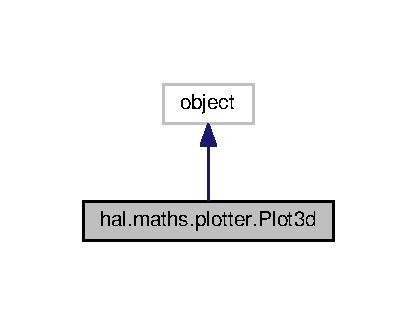
\includegraphics[width=200pt]{classhal_1_1maths_1_1plotter_1_1_plot3d__inherit__graph}
\end{center}
\end{figure}


Collaboration diagram for hal.\+maths.\+plotter.\+Plot3d\+:\nopagebreak
\begin{figure}[H]
\begin{center}
\leavevmode
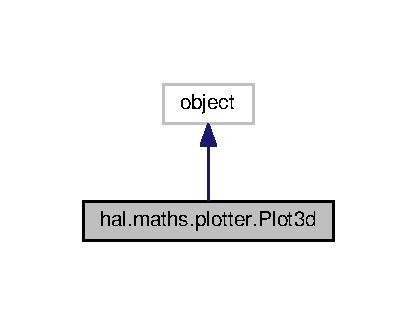
\includegraphics[width=200pt]{classhal_1_1maths_1_1plotter_1_1_plot3d__coll__graph}
\end{center}
\end{figure}
\subsection*{Public Member Functions}
\begin{DoxyCompactItemize}
\item 
def \hyperlink{classhal_1_1maths_1_1plotter_1_1_plot3d_ad17823fc8ceb91fa2c602c45f8eae70e}{param} (self, functionx, functiony, functionz, min, max, points)
\item 
def \hyperlink{classhal_1_1maths_1_1plotter_1_1_plot3d_a1e249de9ab5dac1acc94f82bada6deb0}{plot} (self, function, minx, maxx, pointsx, miny, maxy, pointsy)
\end{DoxyCompactItemize}
\subsection*{Static Public Member Functions}
\begin{DoxyCompactItemize}
\item 
def \hyperlink{classhal_1_1maths_1_1plotter_1_1_plot3d_ac426f777196d1c85ae841e59ea43ad89}{scatter} (vectorx, vectory, vectorz)
\end{DoxyCompactItemize}


\subsection{Member Function Documentation}
\index{hal\+::maths\+::plotter\+::\+Plot3d@{hal\+::maths\+::plotter\+::\+Plot3d}!param@{param}}
\index{param@{param}!hal\+::maths\+::plotter\+::\+Plot3d@{hal\+::maths\+::plotter\+::\+Plot3d}}
\subsubsection[{\texorpdfstring{param(self, functionx, functiony, functionz, min, max, points)}{param(self, functionx, functiony, functionz, min, max, points)}}]{\setlength{\rightskip}{0pt plus 5cm}def hal.\+maths.\+plotter.\+Plot3d.\+param (
\begin{DoxyParamCaption}
\item[{}]{self, }
\item[{}]{functionx, }
\item[{}]{functiony, }
\item[{}]{functionz, }
\item[{}]{min, }
\item[{}]{max, }
\item[{}]{points}
\end{DoxyParamCaption}
)}\hypertarget{classhal_1_1maths_1_1plotter_1_1_plot3d_ad17823fc8ceb91fa2c602c45f8eae70e}{}\label{classhal_1_1maths_1_1plotter_1_1_plot3d_ad17823fc8ceb91fa2c602c45f8eae70e}
\begin{DoxyVerb}:param functionx: function in x
:param functiony: function in y
:param functionz: function in z
:param min: minimum
:param max: maximum
:param points: number of points
:return: 3d parametric graph of given function from min to max
\end{DoxyVerb}
 \index{hal\+::maths\+::plotter\+::\+Plot3d@{hal\+::maths\+::plotter\+::\+Plot3d}!plot@{plot}}
\index{plot@{plot}!hal\+::maths\+::plotter\+::\+Plot3d@{hal\+::maths\+::plotter\+::\+Plot3d}}
\subsubsection[{\texorpdfstring{plot(self, function, minx, maxx, pointsx, miny, maxy, pointsy)}{plot(self, function, minx, maxx, pointsx, miny, maxy, pointsy)}}]{\setlength{\rightskip}{0pt plus 5cm}def hal.\+maths.\+plotter.\+Plot3d.\+plot (
\begin{DoxyParamCaption}
\item[{}]{self, }
\item[{}]{function, }
\item[{}]{minx, }
\item[{}]{maxx, }
\item[{}]{pointsx, }
\item[{}]{miny, }
\item[{}]{maxy, }
\item[{}]{pointsy}
\end{DoxyParamCaption}
)}\hypertarget{classhal_1_1maths_1_1plotter_1_1_plot3d_a1e249de9ab5dac1acc94f82bada6deb0}{}\label{classhal_1_1maths_1_1plotter_1_1_plot3d_a1e249de9ab5dac1acc94f82bada6deb0}
\begin{DoxyVerb}:param function: function to plot
:param minx: minimum of x-values
:param maxx: maximum of x-values
:param pointsx: points in x axis
:param miny: minimum of y-values
:param maxy: maximum of y-values
:param pointsy: points in y axis
:return: plot 3d function
\end{DoxyVerb}
 \index{hal\+::maths\+::plotter\+::\+Plot3d@{hal\+::maths\+::plotter\+::\+Plot3d}!scatter@{scatter}}
\index{scatter@{scatter}!hal\+::maths\+::plotter\+::\+Plot3d@{hal\+::maths\+::plotter\+::\+Plot3d}}
\subsubsection[{\texorpdfstring{scatter(vectorx, vectory, vectorz)}{scatter(vectorx, vectory, vectorz)}}]{\setlength{\rightskip}{0pt plus 5cm}def hal.\+maths.\+plotter.\+Plot3d.\+scatter (
\begin{DoxyParamCaption}
\item[{}]{vectorx, }
\item[{}]{vectory, }
\item[{}]{vectorz}
\end{DoxyParamCaption}
)\hspace{0.3cm}{\ttfamily [static]}}\hypertarget{classhal_1_1maths_1_1plotter_1_1_plot3d_ac426f777196d1c85ae841e59ea43ad89}{}\label{classhal_1_1maths_1_1plotter_1_1_plot3d_ac426f777196d1c85ae841e59ea43ad89}
\begin{DoxyVerb}:param vectorx: vector in x axis
:param vectory: vector in y axis
:param vectorz: vector in z axis
:return: plot 3d scattered points
\end{DoxyVerb}
 

The documentation for this class was generated from the following file\+:\begin{DoxyCompactItemize}
\item 
/home/stefano/\+Coding/\+Python/projects/pyhal/hal/maths/plotter.\+py\end{DoxyCompactItemize}

\hypertarget{classhal_1_1maths_1_1plotter_1_1_plot4d}{}\section{hal.\+maths.\+plotter.\+Plot4d Class Reference}
\label{classhal_1_1maths_1_1plotter_1_1_plot4d}\index{hal.\+maths.\+plotter.\+Plot4d@{hal.\+maths.\+plotter.\+Plot4d}}


Inheritance diagram for hal.\+maths.\+plotter.\+Plot4d\+:\nopagebreak
\begin{figure}[H]
\begin{center}
\leavevmode
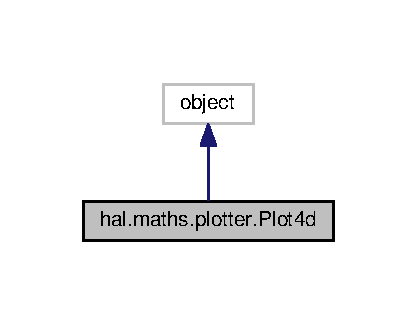
\includegraphics[width=200pt]{classhal_1_1maths_1_1plotter_1_1_plot4d__inherit__graph}
\end{center}
\end{figure}


Collaboration diagram for hal.\+maths.\+plotter.\+Plot4d\+:\nopagebreak
\begin{figure}[H]
\begin{center}
\leavevmode
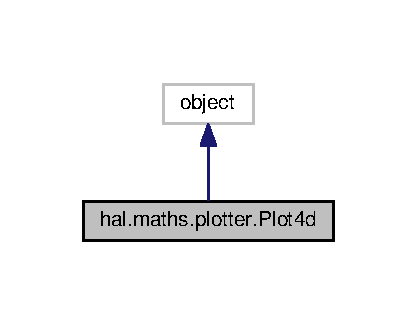
\includegraphics[width=200pt]{classhal_1_1maths_1_1plotter_1_1_plot4d__coll__graph}
\end{center}
\end{figure}
\subsection*{Public Member Functions}
\begin{DoxyCompactItemize}
\item 
def \hyperlink{classhal_1_1maths_1_1plotter_1_1_plot4d_a90b39427c236100f8c080e08e2222f2d}{param} (self, functionx, functiony, functionz, functionw, min, max, points)
\item 
def \hyperlink{classhal_1_1maths_1_1plotter_1_1_plot4d_aa776ce05b0f159953ea817402aa9e280}{plot} (self, function, minx, maxx, miny, maxy, minz, maxz, precision, kind)
\end{DoxyCompactItemize}
\subsection*{Static Public Member Functions}
\begin{DoxyCompactItemize}
\item 
def \hyperlink{classhal_1_1maths_1_1plotter_1_1_plot4d_a1f822a4cfb97006651da35cb2f5e55d1}{scatter} (vectorx, vectory, vectorz, vectorw)
\end{DoxyCompactItemize}


\subsection{Member Function Documentation}
\index{hal\+::maths\+::plotter\+::\+Plot4d@{hal\+::maths\+::plotter\+::\+Plot4d}!param@{param}}
\index{param@{param}!hal\+::maths\+::plotter\+::\+Plot4d@{hal\+::maths\+::plotter\+::\+Plot4d}}
\subsubsection[{\texorpdfstring{param(self, functionx, functiony, functionz, functionw, min, max, points)}{param(self, functionx, functiony, functionz, functionw, min, max, points)}}]{\setlength{\rightskip}{0pt plus 5cm}def hal.\+maths.\+plotter.\+Plot4d.\+param (
\begin{DoxyParamCaption}
\item[{}]{self, }
\item[{}]{functionx, }
\item[{}]{functiony, }
\item[{}]{functionz, }
\item[{}]{functionw, }
\item[{}]{min, }
\item[{}]{max, }
\item[{}]{points}
\end{DoxyParamCaption}
)}\hypertarget{classhal_1_1maths_1_1plotter_1_1_plot4d_a90b39427c236100f8c080e08e2222f2d}{}\label{classhal_1_1maths_1_1plotter_1_1_plot4d_a90b39427c236100f8c080e08e2222f2d}
\begin{DoxyVerb}:param functionx: function in x
:param functiony: function in y
:param functionz: function in z
:param functionw: function in w
:param min: minimum
:param max: maximum
:param points: number of points
:return: 4d parametric graph of given function from min to max
\end{DoxyVerb}
 \index{hal\+::maths\+::plotter\+::\+Plot4d@{hal\+::maths\+::plotter\+::\+Plot4d}!plot@{plot}}
\index{plot@{plot}!hal\+::maths\+::plotter\+::\+Plot4d@{hal\+::maths\+::plotter\+::\+Plot4d}}
\subsubsection[{\texorpdfstring{plot(self, function, minx, maxx, miny, maxy, minz, maxz, precision, kind)}{plot(self, function, minx, maxx, miny, maxy, minz, maxz, precision, kind)}}]{\setlength{\rightskip}{0pt plus 5cm}def hal.\+maths.\+plotter.\+Plot4d.\+plot (
\begin{DoxyParamCaption}
\item[{}]{self, }
\item[{}]{function, }
\item[{}]{minx, }
\item[{}]{maxx, }
\item[{}]{miny, }
\item[{}]{maxy, }
\item[{}]{minz, }
\item[{}]{maxz, }
\item[{}]{precision, }
\item[{}]{kind}
\end{DoxyParamCaption}
)}\hypertarget{classhal_1_1maths_1_1plotter_1_1_plot4d_aa776ce05b0f159953ea817402aa9e280}{}\label{classhal_1_1maths_1_1plotter_1_1_plot4d_aa776ce05b0f159953ea817402aa9e280}
\begin{DoxyVerb}:param function: function to plot
:param minx: minimum of x-values
:param maxx: maximum of x-values
:param miny: minimum of y-values
:param maxy: maximum of y-values
:param minz: minimum of z-values
:param maxz: maximum of z-values
:param precision: precision
:param kind: slice: x cont -> 3d plot with y,z variables in plane and w as "z"-axis
     contour: x cont -> 3d plot with y,z variables in plane and w colored
:return: plot 4d function
\end{DoxyVerb}
 \index{hal\+::maths\+::plotter\+::\+Plot4d@{hal\+::maths\+::plotter\+::\+Plot4d}!scatter@{scatter}}
\index{scatter@{scatter}!hal\+::maths\+::plotter\+::\+Plot4d@{hal\+::maths\+::plotter\+::\+Plot4d}}
\subsubsection[{\texorpdfstring{scatter(vectorx, vectory, vectorz, vectorw)}{scatter(vectorx, vectory, vectorz, vectorw)}}]{\setlength{\rightskip}{0pt plus 5cm}def hal.\+maths.\+plotter.\+Plot4d.\+scatter (
\begin{DoxyParamCaption}
\item[{}]{vectorx, }
\item[{}]{vectory, }
\item[{}]{vectorz, }
\item[{}]{vectorw}
\end{DoxyParamCaption}
)\hspace{0.3cm}{\ttfamily [static]}}\hypertarget{classhal_1_1maths_1_1plotter_1_1_plot4d_a1f822a4cfb97006651da35cb2f5e55d1}{}\label{classhal_1_1maths_1_1plotter_1_1_plot4d_a1f822a4cfb97006651da35cb2f5e55d1}
\begin{DoxyVerb}:param vectorx: vector in x axis
:param vectory: vector in y axis
:param vectorz: vector in z axis
:param vectorw: vector in w axis
:return: plot 4d scattered points
\end{DoxyVerb}
 

The documentation for this class was generated from the following file\+:\begin{DoxyCompactItemize}
\item 
/home/stefano/\+Coding/\+Python/projects/pyhal/hal/maths/plotter.\+py\end{DoxyCompactItemize}

\hypertarget{classhal_1_1internet_1_1engines_1_1_search_engine}{}\section{hal.\+internet.\+engines.\+Search\+Engine Class Reference}
\label{classhal_1_1internet_1_1engines_1_1_search_engine}\index{hal.\+internet.\+engines.\+Search\+Engine@{hal.\+internet.\+engines.\+Search\+Engine}}


Inheritance diagram for hal.\+internet.\+engines.\+Search\+Engine\+:\nopagebreak
\begin{figure}[H]
\begin{center}
\leavevmode
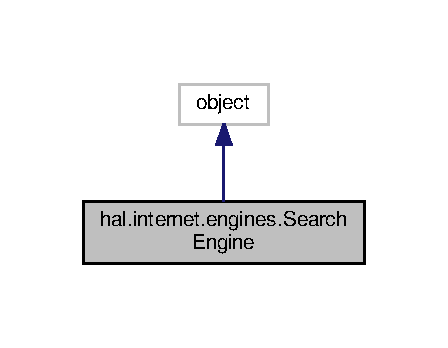
\includegraphics[width=215pt]{classhal_1_1internet_1_1engines_1_1_search_engine__inherit__graph}
\end{center}
\end{figure}


Collaboration diagram for hal.\+internet.\+engines.\+Search\+Engine\+:\nopagebreak
\begin{figure}[H]
\begin{center}
\leavevmode
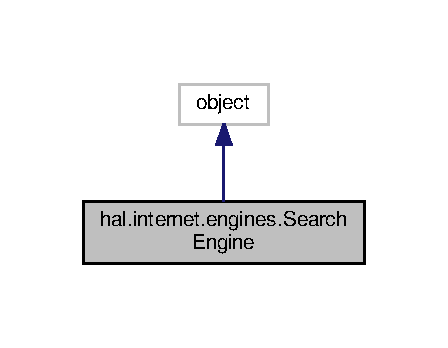
\includegraphics[width=215pt]{classhal_1_1internet_1_1engines_1_1_search_engine__coll__graph}
\end{center}
\end{figure}
\subsection*{Public Member Functions}
\begin{DoxyCompactItemize}
\item 
def \hyperlink{classhal_1_1internet_1_1engines_1_1_search_engine_afa48d729c2ecd0ba30a56544dd3951ea}{\+\_\+\+\_\+init\+\_\+\+\_\+} (self, url, blank\+\_\+replace=\char`\"{}+\char`\"{})
\item 
def \hyperlink{classhal_1_1internet_1_1engines_1_1_search_engine_afde9fa1646b6057ecd94746132c9b7c1}{parse\+\_\+query} (self, query)
\item 
def \hyperlink{classhal_1_1internet_1_1engines_1_1_search_engine_a05d68c392a6d698cd59df41927ddbc90}{get\+\_\+search\+\_\+page} (self, query, using\+\_\+tor=False)
\end{DoxyCompactItemize}
\subsection*{Public Attributes}
\begin{DoxyCompactItemize}
\item 
{\bfseries url}\hypertarget{classhal_1_1internet_1_1engines_1_1_search_engine_a2b16e6f92de3d9dd64d1c51efbd8717d}{}\label{classhal_1_1internet_1_1engines_1_1_search_engine_a2b16e6f92de3d9dd64d1c51efbd8717d}

\item 
{\bfseries web\+\_\+page}\hypertarget{classhal_1_1internet_1_1engines_1_1_search_engine_abb2f49a429aa664261c55de3a953b7ce}{}\label{classhal_1_1internet_1_1engines_1_1_search_engine_abb2f49a429aa664261c55de3a953b7ce}

\item 
{\bfseries domain}\hypertarget{classhal_1_1internet_1_1engines_1_1_search_engine_a96f97387f7a035a12cb1509288b5401a}{}\label{classhal_1_1internet_1_1engines_1_1_search_engine_a96f97387f7a035a12cb1509288b5401a}

\item 
{\bfseries blank\+\_\+replace}\hypertarget{classhal_1_1internet_1_1engines_1_1_search_engine_a28184626d85a0e6a0af8f3a2e381cf7f}{}\label{classhal_1_1internet_1_1engines_1_1_search_engine_a28184626d85a0e6a0af8f3a2e381cf7f}

\end{DoxyCompactItemize}


\subsection{Detailed Description}
\begin{DoxyVerb}Internet general search engine \end{DoxyVerb}
 

\subsection{Constructor \& Destructor Documentation}
\index{hal\+::internet\+::engines\+::\+Search\+Engine@{hal\+::internet\+::engines\+::\+Search\+Engine}!\+\_\+\+\_\+init\+\_\+\+\_\+@{\+\_\+\+\_\+init\+\_\+\+\_\+}}
\index{\+\_\+\+\_\+init\+\_\+\+\_\+@{\+\_\+\+\_\+init\+\_\+\+\_\+}!hal\+::internet\+::engines\+::\+Search\+Engine@{hal\+::internet\+::engines\+::\+Search\+Engine}}
\subsubsection[{\texorpdfstring{\+\_\+\+\_\+init\+\_\+\+\_\+(self, url, blank\+\_\+replace=""+"")}{__init__(self, url, blank_replace="+")}}]{\setlength{\rightskip}{0pt plus 5cm}def hal.\+internet.\+engines.\+Search\+Engine.\+\_\+\+\_\+init\+\_\+\+\_\+ (
\begin{DoxyParamCaption}
\item[{}]{self, }
\item[{}]{url, }
\item[{}]{blank\+\_\+replace = {\ttfamily \char`\"{}+\char`\"{}}}
\end{DoxyParamCaption}
)}\hypertarget{classhal_1_1internet_1_1engines_1_1_search_engine_afa48d729c2ecd0ba30a56544dd3951ea}{}\label{classhal_1_1internet_1_1engines_1_1_search_engine_afa48d729c2ecd0ba30a56544dd3951ea}
\begin{DoxyVerb}:param url: string
    Url of search engine used in all query.
:param blank_replace:
    Every search engine has to replace blanks in query
\end{DoxyVerb}
 

\subsection{Member Function Documentation}
\index{hal\+::internet\+::engines\+::\+Search\+Engine@{hal\+::internet\+::engines\+::\+Search\+Engine}!get\+\_\+search\+\_\+page@{get\+\_\+search\+\_\+page}}
\index{get\+\_\+search\+\_\+page@{get\+\_\+search\+\_\+page}!hal\+::internet\+::engines\+::\+Search\+Engine@{hal\+::internet\+::engines\+::\+Search\+Engine}}
\subsubsection[{\texorpdfstring{get\+\_\+search\+\_\+page(self, query, using\+\_\+tor=\+False)}{get_search_page(self, query, using_tor=False)}}]{\setlength{\rightskip}{0pt plus 5cm}def hal.\+internet.\+engines.\+Search\+Engine.\+get\+\_\+search\+\_\+page (
\begin{DoxyParamCaption}
\item[{}]{self, }
\item[{}]{query, }
\item[{}]{using\+\_\+tor = {\ttfamily False}}
\end{DoxyParamCaption}
)}\hypertarget{classhal_1_1internet_1_1engines_1_1_search_engine_a05d68c392a6d698cd59df41927ddbc90}{}\label{classhal_1_1internet_1_1engines_1_1_search_engine_a05d68c392a6d698cd59df41927ddbc90}
\begin{DoxyVerb}:param query: string
    Query to search engine.
:param using_tor: bool
    Whether use tor or not to fetch web pages
:return: string
    Get HTML source of search page of given query.
\end{DoxyVerb}
 \index{hal\+::internet\+::engines\+::\+Search\+Engine@{hal\+::internet\+::engines\+::\+Search\+Engine}!parse\+\_\+query@{parse\+\_\+query}}
\index{parse\+\_\+query@{parse\+\_\+query}!hal\+::internet\+::engines\+::\+Search\+Engine@{hal\+::internet\+::engines\+::\+Search\+Engine}}
\subsubsection[{\texorpdfstring{parse\+\_\+query(self, query)}{parse_query(self, query)}}]{\setlength{\rightskip}{0pt plus 5cm}def hal.\+internet.\+engines.\+Search\+Engine.\+parse\+\_\+query (
\begin{DoxyParamCaption}
\item[{}]{self, }
\item[{}]{query}
\end{DoxyParamCaption}
)}\hypertarget{classhal_1_1internet_1_1engines_1_1_search_engine_afde9fa1646b6057ecd94746132c9b7c1}{}\label{classhal_1_1internet_1_1engines_1_1_search_engine_afde9fa1646b6057ecd94746132c9b7c1}
\begin{DoxyVerb}:param query: string
    Query to search engine.
:return: string
    Parse given query in order to meet search criteria of search engine
\end{DoxyVerb}
 

The documentation for this class was generated from the following file\+:\begin{DoxyCompactItemize}
\item 
/home/stefano/\+Coding/\+Python/projects/pyhal/hal/internet/engines.\+py\end{DoxyCompactItemize}

\hypertarget{classhal_1_1internet_1_1engines_1_1_search_engine_result}{}\section{hal.\+internet.\+engines.\+Search\+Engine\+Result Class Reference}
\label{classhal_1_1internet_1_1engines_1_1_search_engine_result}\index{hal.\+internet.\+engines.\+Search\+Engine\+Result@{hal.\+internet.\+engines.\+Search\+Engine\+Result}}


Inheritance diagram for hal.\+internet.\+engines.\+Search\+Engine\+Result\+:
\nopagebreak
\begin{figure}[H]
\begin{center}
\leavevmode
\includegraphics[width=215pt]{classhal_1_1internet_1_1engines_1_1_search_engine_result__inherit__graph}
\end{center}
\end{figure}


Collaboration diagram for hal.\+internet.\+engines.\+Search\+Engine\+Result\+:
\nopagebreak
\begin{figure}[H]
\begin{center}
\leavevmode
\includegraphics[width=215pt]{classhal_1_1internet_1_1engines_1_1_search_engine_result__coll__graph}
\end{center}
\end{figure}
\subsection*{Public Member Functions}
\begin{DoxyCompactItemize}
\item 
def {\bfseries \+\_\+\+\_\+init\+\_\+\+\_\+} (self, title, link, description=\char`\"{}\char`\"{})\hypertarget{classhal_1_1internet_1_1engines_1_1_search_engine_result_aafeb2e635cb5a9b381d5535c714d11c2}{}\label{classhal_1_1internet_1_1engines_1_1_search_engine_result_aafeb2e635cb5a9b381d5535c714d11c2}

\item 
def {\bfseries \+\_\+\+\_\+str\+\_\+\+\_\+} (self)\hypertarget{classhal_1_1internet_1_1engines_1_1_search_engine_result_aa65111d2c02c5e1d9d2b135d60eaeeac}{}\label{classhal_1_1internet_1_1engines_1_1_search_engine_result_aa65111d2c02c5e1d9d2b135d60eaeeac}

\end{DoxyCompactItemize}
\subsection*{Public Attributes}
\begin{DoxyCompactItemize}
\item 
{\bfseries title}\hypertarget{classhal_1_1internet_1_1engines_1_1_search_engine_result_ad5bf472925c771cddddc1ec8008cc6b2}{}\label{classhal_1_1internet_1_1engines_1_1_search_engine_result_ad5bf472925c771cddddc1ec8008cc6b2}

\item 
{\bfseries link}\hypertarget{classhal_1_1internet_1_1engines_1_1_search_engine_result_a87fd88d4579dd7be2fed559386cc58e8}{}\label{classhal_1_1internet_1_1engines_1_1_search_engine_result_a87fd88d4579dd7be2fed559386cc58e8}

\item 
{\bfseries description}\hypertarget{classhal_1_1internet_1_1engines_1_1_search_engine_result_a055578b70da89ea3248abb6aa27d92df}{}\label{classhal_1_1internet_1_1engines_1_1_search_engine_result_a055578b70da89ea3248abb6aa27d92df}

\end{DoxyCompactItemize}


The documentation for this class was generated from the following file\+:\begin{DoxyCompactItemize}
\item 
hal/internet/engines.\+py\end{DoxyCompactItemize}

\hypertarget{classhal_1_1internet_1_1selenium_1_1_selenium_form}{}\section{hal.\+internet.\+selenium.\+Selenium\+Form Class Reference}
\label{classhal_1_1internet_1_1selenium_1_1_selenium_form}\index{hal.\+internet.\+selenium.\+Selenium\+Form@{hal.\+internet.\+selenium.\+Selenium\+Form}}
\subsection*{Static Public Member Functions}
\begin{DoxyCompactItemize}
\item 
def \hyperlink{classhal_1_1internet_1_1selenium_1_1_selenium_form_a9523968c9daa9a96f9a7b7ddd358904b}{fill\+\_\+form\+\_\+field} (browser, field\+\_\+name, field\+\_\+value)
\item 
def \hyperlink{classhal_1_1internet_1_1selenium_1_1_selenium_form_aa73bb0384f074f2d1b07f78c7bfb6867}{fill\+\_\+login\+\_\+form} (browser, username, username\+\_\+field, userpassword, userpassword\+\_\+field)
\item 
def \hyperlink{classhal_1_1internet_1_1selenium_1_1_selenium_form_a7648cf31df2f596b9af4f9b9583f2bdb}{submit\+\_\+form} (browser, button\+\_\+name)
\end{DoxyCompactItemize}


\subsection{Detailed Description}
\begin{DoxyVerb}Great and simple static methods to deal with selenium webdrivers. \end{DoxyVerb}
 

\subsection{Member Function Documentation}
\index{hal\+::internet\+::selenium\+::\+Selenium\+Form@{hal\+::internet\+::selenium\+::\+Selenium\+Form}!fill\+\_\+form\+\_\+field@{fill\+\_\+form\+\_\+field}}
\index{fill\+\_\+form\+\_\+field@{fill\+\_\+form\+\_\+field}!hal\+::internet\+::selenium\+::\+Selenium\+Form@{hal\+::internet\+::selenium\+::\+Selenium\+Form}}
\subsubsection[{\texorpdfstring{fill\+\_\+form\+\_\+field(browser, field\+\_\+name, field\+\_\+value)}{fill_form_field(browser, field_name, field_value)}}]{\setlength{\rightskip}{0pt plus 5cm}def hal.\+internet.\+selenium.\+Selenium\+Form.\+fill\+\_\+form\+\_\+field (
\begin{DoxyParamCaption}
\item[{}]{browser, }
\item[{}]{field\+\_\+name, }
\item[{}]{field\+\_\+value}
\end{DoxyParamCaption}
)\hspace{0.3cm}{\ttfamily [static]}}\hypertarget{classhal_1_1internet_1_1selenium_1_1_selenium_form_a9523968c9daa9a96f9a7b7ddd358904b}{}\label{classhal_1_1internet_1_1selenium_1_1_selenium_form_a9523968c9daa9a96f9a7b7ddd358904b}
\begin{DoxyVerb}:param browser: webdriver
    Browser to use to submit form.
:param field_name :string
    Name of field to fill
:param field_value: string
    Value with which to fill field.
:return: void
    Fill given field wiht given value.
\end{DoxyVerb}
 \index{hal\+::internet\+::selenium\+::\+Selenium\+Form@{hal\+::internet\+::selenium\+::\+Selenium\+Form}!fill\+\_\+login\+\_\+form@{fill\+\_\+login\+\_\+form}}
\index{fill\+\_\+login\+\_\+form@{fill\+\_\+login\+\_\+form}!hal\+::internet\+::selenium\+::\+Selenium\+Form@{hal\+::internet\+::selenium\+::\+Selenium\+Form}}
\subsubsection[{\texorpdfstring{fill\+\_\+login\+\_\+form(browser, username, username\+\_\+field, userpassword, userpassword\+\_\+field)}{fill_login_form(browser, username, username_field, userpassword, userpassword_field)}}]{\setlength{\rightskip}{0pt plus 5cm}def hal.\+internet.\+selenium.\+Selenium\+Form.\+fill\+\_\+login\+\_\+form (
\begin{DoxyParamCaption}
\item[{}]{browser, }
\item[{}]{username, }
\item[{}]{username\+\_\+field, }
\item[{}]{userpassword, }
\item[{}]{userpassword\+\_\+field}
\end{DoxyParamCaption}
)\hspace{0.3cm}{\ttfamily [static]}}\hypertarget{classhal_1_1internet_1_1selenium_1_1_selenium_form_aa73bb0384f074f2d1b07f78c7bfb6867}{}\label{classhal_1_1internet_1_1selenium_1_1_selenium_form_aa73bb0384f074f2d1b07f78c7bfb6867}
\begin{DoxyVerb}:param browser: webdriver
    Browser to use to submit form.
:param username: string
    Username of user to login.
:param username_field: string
    Name of field to fill with username.
:param userpassword: string
    Password of user to login.
:param userpassword_field: string
    Name of field to fill with userpassword.
:return: void
    Form filled with given information.
\end{DoxyVerb}
 \index{hal\+::internet\+::selenium\+::\+Selenium\+Form@{hal\+::internet\+::selenium\+::\+Selenium\+Form}!submit\+\_\+form@{submit\+\_\+form}}
\index{submit\+\_\+form@{submit\+\_\+form}!hal\+::internet\+::selenium\+::\+Selenium\+Form@{hal\+::internet\+::selenium\+::\+Selenium\+Form}}
\subsubsection[{\texorpdfstring{submit\+\_\+form(browser, button\+\_\+name)}{submit_form(browser, button_name)}}]{\setlength{\rightskip}{0pt plus 5cm}def hal.\+internet.\+selenium.\+Selenium\+Form.\+submit\+\_\+form (
\begin{DoxyParamCaption}
\item[{}]{browser, }
\item[{}]{button\+\_\+name}
\end{DoxyParamCaption}
)\hspace{0.3cm}{\ttfamily [static]}}\hypertarget{classhal_1_1internet_1_1selenium_1_1_selenium_form_a7648cf31df2f596b9af4f9b9583f2bdb}{}\label{classhal_1_1internet_1_1selenium_1_1_selenium_form_a7648cf31df2f596b9af4f9b9583f2bdb}
\begin{DoxyVerb}:param browser: webdriver
    Browser to use to submit form.
:param button_name: string
    Name of button to press to submit form
:return: void
    Submit form.
\end{DoxyVerb}
 

The documentation for this class was generated from the following file\+:\begin{DoxyCompactItemize}
\item 
hal/internet/selenium.\+py\end{DoxyCompactItemize}

\hypertarget{classhal_1_1maths_1_1crypt_1_1_s_h_a}{}\section{hal.\+maths.\+crypt.\+S\+HA Class Reference}
\label{classhal_1_1maths_1_1crypt_1_1_s_h_a}\index{hal.\+maths.\+crypt.\+S\+HA@{hal.\+maths.\+crypt.\+S\+HA}}


Inheritance diagram for hal.\+maths.\+crypt.\+S\+HA\+:\nopagebreak
\begin{figure}[H]
\begin{center}
\leavevmode
\includegraphics[width=188pt]{classhal_1_1maths_1_1crypt_1_1_s_h_a__inherit__graph}
\end{center}
\end{figure}


Collaboration diagram for hal.\+maths.\+crypt.\+S\+HA\+:\nopagebreak
\begin{figure}[H]
\begin{center}
\leavevmode
\includegraphics[width=188pt]{classhal_1_1maths_1_1crypt_1_1_s_h_a__coll__graph}
\end{center}
\end{figure}
\subsection*{Public Member Functions}
\begin{DoxyCompactItemize}
\item 
def {\bfseries \+\_\+\+\_\+init\+\_\+\+\_\+} (self, string, size, salt=None)\hypertarget{classhal_1_1maths_1_1crypt_1_1_s_h_a_accde1fc65395f7ecd7869fa7a71961f1}{}\label{classhal_1_1maths_1_1crypt_1_1_s_h_a_accde1fc65395f7ecd7869fa7a71961f1}

\item 
def \hyperlink{classhal_1_1maths_1_1crypt_1_1_s_h_a_a4434870473a585d5382945a8cef6c7c3}{hash} (self)
\item 
def \hyperlink{classhal_1_1maths_1_1crypt_1_1_s_h_a_a87af3f937c0cfed513ea0720c4814246}{hash\+\_\+sha1} (self)
\item 
def \hyperlink{classhal_1_1maths_1_1crypt_1_1_s_h_a_ad258fade71cc488adc9e5cbcfaf7fc9c}{hash\+\_\+sha224} (self)
\item 
def \hyperlink{classhal_1_1maths_1_1crypt_1_1_s_h_a_aa2c42ae578cf76dc73cfd443fc931605}{hash\+\_\+sha256} (self)
\item 
def \hyperlink{classhal_1_1maths_1_1crypt_1_1_s_h_a_af0a05dbeeb0ec1f6530aa8c99937b44f}{hash\+\_\+sha384} (self)
\item 
def \hyperlink{classhal_1_1maths_1_1crypt_1_1_s_h_a_ad799ad40338287efb2a6f539954d35e9}{hash\+\_\+sha512} (self)
\item 
def \hyperlink{classhal_1_1maths_1_1crypt_1_1_s_h_a_a9ebefcb7012b2b306cd6b70feb646d8c}{hash\+\_\+shasalted} (self)
\end{DoxyCompactItemize}
\subsection*{Public Attributes}
\begin{DoxyCompactItemize}
\item 
{\bfseries plain}\hypertarget{classhal_1_1maths_1_1crypt_1_1_s_h_a_ad683af29f5abcb0607b3152750ed2848}{}\label{classhal_1_1maths_1_1crypt_1_1_s_h_a_ad683af29f5abcb0607b3152750ed2848}

\item 
{\bfseries size}\hypertarget{classhal_1_1maths_1_1crypt_1_1_s_h_a_a039dcc420e588091d5bf74037882ec31}{}\label{classhal_1_1maths_1_1crypt_1_1_s_h_a_a039dcc420e588091d5bf74037882ec31}

\item 
{\bfseries salt}\hypertarget{classhal_1_1maths_1_1crypt_1_1_s_h_a_ad0916d65406b116f81a23754a3ca3c79}{}\label{classhal_1_1maths_1_1crypt_1_1_s_h_a_ad0916d65406b116f81a23754a3ca3c79}

\item 
{\bfseries hashed}\hypertarget{classhal_1_1maths_1_1crypt_1_1_s_h_a_a633832075c61a928b02a9a9c0fa133eb}{}\label{classhal_1_1maths_1_1crypt_1_1_s_h_a_a633832075c61a928b02a9a9c0fa133eb}

\end{DoxyCompactItemize}
\subsection*{Static Public Attributes}
\begin{DoxyCompactItemize}
\item 
list {\bfseries A\+L\+L\+O\+W\+E\+D\+\_\+\+S\+I\+ZE} = \mbox{[}1, 224, 256, 384, 512\mbox{]}\hypertarget{classhal_1_1maths_1_1crypt_1_1_s_h_a_ac548ef72156aee09835369f224ba1349}{}\label{classhal_1_1maths_1_1crypt_1_1_s_h_a_ac548ef72156aee09835369f224ba1349}

\end{DoxyCompactItemize}


\subsection{Detailed Description}
\begin{DoxyVerb}general SHA hash \end{DoxyVerb}
 

\subsection{Member Function Documentation}
\index{hal\+::maths\+::crypt\+::\+S\+HA@{hal\+::maths\+::crypt\+::\+S\+HA}!hash@{hash}}
\index{hash@{hash}!hal\+::maths\+::crypt\+::\+S\+HA@{hal\+::maths\+::crypt\+::\+S\+HA}}
\subsubsection[{\texorpdfstring{hash(self)}{hash(self)}}]{\setlength{\rightskip}{0pt plus 5cm}def hal.\+maths.\+crypt.\+S\+H\+A.\+hash (
\begin{DoxyParamCaption}
\item[{}]{self}
\end{DoxyParamCaption}
)}\hypertarget{classhal_1_1maths_1_1crypt_1_1_s_h_a_a4434870473a585d5382945a8cef6c7c3}{}\label{classhal_1_1maths_1_1crypt_1_1_s_h_a_a4434870473a585d5382945a8cef6c7c3}
\begin{DoxyVerb}:return: hash of given size
\end{DoxyVerb}
 \index{hal\+::maths\+::crypt\+::\+S\+HA@{hal\+::maths\+::crypt\+::\+S\+HA}!hash\+\_\+sha1@{hash\+\_\+sha1}}
\index{hash\+\_\+sha1@{hash\+\_\+sha1}!hal\+::maths\+::crypt\+::\+S\+HA@{hal\+::maths\+::crypt\+::\+S\+HA}}
\subsubsection[{\texorpdfstring{hash\+\_\+sha1(self)}{hash_sha1(self)}}]{\setlength{\rightskip}{0pt plus 5cm}def hal.\+maths.\+crypt.\+S\+H\+A.\+hash\+\_\+sha1 (
\begin{DoxyParamCaption}
\item[{}]{self}
\end{DoxyParamCaption}
)}\hypertarget{classhal_1_1maths_1_1crypt_1_1_s_h_a_a87af3f937c0cfed513ea0720c4814246}{}\label{classhal_1_1maths_1_1crypt_1_1_s_h_a_a87af3f937c0cfed513ea0720c4814246}
\begin{DoxyVerb}:return: sha1 hash
\end{DoxyVerb}
 \index{hal\+::maths\+::crypt\+::\+S\+HA@{hal\+::maths\+::crypt\+::\+S\+HA}!hash\+\_\+sha224@{hash\+\_\+sha224}}
\index{hash\+\_\+sha224@{hash\+\_\+sha224}!hal\+::maths\+::crypt\+::\+S\+HA@{hal\+::maths\+::crypt\+::\+S\+HA}}
\subsubsection[{\texorpdfstring{hash\+\_\+sha224(self)}{hash_sha224(self)}}]{\setlength{\rightskip}{0pt plus 5cm}def hal.\+maths.\+crypt.\+S\+H\+A.\+hash\+\_\+sha224 (
\begin{DoxyParamCaption}
\item[{}]{self}
\end{DoxyParamCaption}
)}\hypertarget{classhal_1_1maths_1_1crypt_1_1_s_h_a_ad258fade71cc488adc9e5cbcfaf7fc9c}{}\label{classhal_1_1maths_1_1crypt_1_1_s_h_a_ad258fade71cc488adc9e5cbcfaf7fc9c}
\begin{DoxyVerb}:return: sha224 hash
\end{DoxyVerb}
 \index{hal\+::maths\+::crypt\+::\+S\+HA@{hal\+::maths\+::crypt\+::\+S\+HA}!hash\+\_\+sha256@{hash\+\_\+sha256}}
\index{hash\+\_\+sha256@{hash\+\_\+sha256}!hal\+::maths\+::crypt\+::\+S\+HA@{hal\+::maths\+::crypt\+::\+S\+HA}}
\subsubsection[{\texorpdfstring{hash\+\_\+sha256(self)}{hash_sha256(self)}}]{\setlength{\rightskip}{0pt plus 5cm}def hal.\+maths.\+crypt.\+S\+H\+A.\+hash\+\_\+sha256 (
\begin{DoxyParamCaption}
\item[{}]{self}
\end{DoxyParamCaption}
)}\hypertarget{classhal_1_1maths_1_1crypt_1_1_s_h_a_aa2c42ae578cf76dc73cfd443fc931605}{}\label{classhal_1_1maths_1_1crypt_1_1_s_h_a_aa2c42ae578cf76dc73cfd443fc931605}
\begin{DoxyVerb}:return: sha256 hash
\end{DoxyVerb}
 \index{hal\+::maths\+::crypt\+::\+S\+HA@{hal\+::maths\+::crypt\+::\+S\+HA}!hash\+\_\+sha384@{hash\+\_\+sha384}}
\index{hash\+\_\+sha384@{hash\+\_\+sha384}!hal\+::maths\+::crypt\+::\+S\+HA@{hal\+::maths\+::crypt\+::\+S\+HA}}
\subsubsection[{\texorpdfstring{hash\+\_\+sha384(self)}{hash_sha384(self)}}]{\setlength{\rightskip}{0pt plus 5cm}def hal.\+maths.\+crypt.\+S\+H\+A.\+hash\+\_\+sha384 (
\begin{DoxyParamCaption}
\item[{}]{self}
\end{DoxyParamCaption}
)}\hypertarget{classhal_1_1maths_1_1crypt_1_1_s_h_a_af0a05dbeeb0ec1f6530aa8c99937b44f}{}\label{classhal_1_1maths_1_1crypt_1_1_s_h_a_af0a05dbeeb0ec1f6530aa8c99937b44f}
\begin{DoxyVerb}:return: sha384 hash
\end{DoxyVerb}
 \index{hal\+::maths\+::crypt\+::\+S\+HA@{hal\+::maths\+::crypt\+::\+S\+HA}!hash\+\_\+sha512@{hash\+\_\+sha512}}
\index{hash\+\_\+sha512@{hash\+\_\+sha512}!hal\+::maths\+::crypt\+::\+S\+HA@{hal\+::maths\+::crypt\+::\+S\+HA}}
\subsubsection[{\texorpdfstring{hash\+\_\+sha512(self)}{hash_sha512(self)}}]{\setlength{\rightskip}{0pt plus 5cm}def hal.\+maths.\+crypt.\+S\+H\+A.\+hash\+\_\+sha512 (
\begin{DoxyParamCaption}
\item[{}]{self}
\end{DoxyParamCaption}
)}\hypertarget{classhal_1_1maths_1_1crypt_1_1_s_h_a_ad799ad40338287efb2a6f539954d35e9}{}\label{classhal_1_1maths_1_1crypt_1_1_s_h_a_ad799ad40338287efb2a6f539954d35e9}
\begin{DoxyVerb}:return: sha512 hash
\end{DoxyVerb}
 \index{hal\+::maths\+::crypt\+::\+S\+HA@{hal\+::maths\+::crypt\+::\+S\+HA}!hash\+\_\+shasalted@{hash\+\_\+shasalted}}
\index{hash\+\_\+shasalted@{hash\+\_\+shasalted}!hal\+::maths\+::crypt\+::\+S\+HA@{hal\+::maths\+::crypt\+::\+S\+HA}}
\subsubsection[{\texorpdfstring{hash\+\_\+shasalted(self)}{hash_shasalted(self)}}]{\setlength{\rightskip}{0pt plus 5cm}def hal.\+maths.\+crypt.\+S\+H\+A.\+hash\+\_\+shasalted (
\begin{DoxyParamCaption}
\item[{}]{self}
\end{DoxyParamCaption}
)}\hypertarget{classhal_1_1maths_1_1crypt_1_1_s_h_a_a9ebefcb7012b2b306cd6b70feb646d8c}{}\label{classhal_1_1maths_1_1crypt_1_1_s_h_a_a9ebefcb7012b2b306cd6b70feb646d8c}
\begin{DoxyVerb}:return: sha512 hash
\end{DoxyVerb}
 

The documentation for this class was generated from the following file\+:\begin{DoxyCompactItemize}
\item 
/home/stefano/\+Coding/\+Python/projects/pyhal/hal/maths/crypt.\+py\end{DoxyCompactItemize}

\hypertarget{classhal_1_1internet_1_1web_1_1_webpage}{}\section{hal.\+internet.\+web.\+Webpage Class Reference}
\label{classhal_1_1internet_1_1web_1_1_webpage}\index{hal.\+internet.\+web.\+Webpage@{hal.\+internet.\+web.\+Webpage}}


Inheritance diagram for hal.\+internet.\+web.\+Webpage\+:\nopagebreak
\begin{figure}[H]
\begin{center}
\leavevmode
\includegraphics[width=210pt]{classhal_1_1internet_1_1web_1_1_webpage__inherit__graph}
\end{center}
\end{figure}


Collaboration diagram for hal.\+internet.\+web.\+Webpage\+:\nopagebreak
\begin{figure}[H]
\begin{center}
\leavevmode
\includegraphics[width=210pt]{classhal_1_1internet_1_1web_1_1_webpage__coll__graph}
\end{center}
\end{figure}
\subsection*{Public Member Functions}
\begin{DoxyCompactItemize}
\item 
def \hyperlink{classhal_1_1internet_1_1web_1_1_webpage_abdd82419586ce1fab58d0d594a4780f8}{\+\_\+\+\_\+init\+\_\+\+\_\+} (self, url, using\+\_\+tor=False)
\item 
def \hyperlink{classhal_1_1internet_1_1web_1_1_webpage_a8a5f45d640b9a433fdd4ab4956141ed0}{get\+\_\+scheme} (self)
\item 
def \hyperlink{classhal_1_1internet_1_1web_1_1_webpage_ad3059e24c2ea962b13944209e086b1c8}{get\+\_\+hostname} (self)
\item 
def \hyperlink{classhal_1_1internet_1_1web_1_1_webpage_a1879c8695e4e1c7c0155d24100fbbbc0}{get\+\_\+domain} (self)
\item 
def \hyperlink{classhal_1_1internet_1_1web_1_1_webpage_ad813eba8e41c06f110311ada3ae86f2c}{get\+\_\+html\+\_\+source} (self, tor=False)
\item 
def \hyperlink{classhal_1_1internet_1_1web_1_1_webpage_a73b639e5eaa4506a653c9a4792f7dead}{get\+\_\+links} (self, recall, timeout)
\item 
def \hyperlink{classhal_1_1internet_1_1web_1_1_webpage_ae3904bbb1924178180ca32e922bbbeb5}{open\+\_\+in\+\_\+browser} (self, times)
\end{DoxyCompactItemize}
\subsection*{Static Public Member Functions}
\begin{DoxyCompactItemize}
\item 
def \hyperlink{classhal_1_1internet_1_1web_1_1_webpage_af6e3dcd4dbebe8e1b196fded24e4025e}{parse\+\_\+url} (raw\+\_\+url)
\end{DoxyCompactItemize}
\subsection*{Public Attributes}
\begin{DoxyCompactItemize}
\item 
{\bfseries url}\hypertarget{classhal_1_1internet_1_1web_1_1_webpage_a9daf360debee3008329bcd28c0e578ed}{}\label{classhal_1_1internet_1_1web_1_1_webpage_a9daf360debee3008329bcd28c0e578ed}

\item 
{\bfseries domain}\hypertarget{classhal_1_1internet_1_1web_1_1_webpage_a0440d1bfe5d1a8e510d8ac3254731846}{}\label{classhal_1_1internet_1_1web_1_1_webpage_a0440d1bfe5d1a8e510d8ac3254731846}

\item 
{\bfseries using\+\_\+tor}\hypertarget{classhal_1_1internet_1_1web_1_1_webpage_a7320808ec3b5ad1a2b8f30dd10d50229}{}\label{classhal_1_1internet_1_1web_1_1_webpage_a7320808ec3b5ad1a2b8f30dd10d50229}

\item 
{\bfseries source}\hypertarget{classhal_1_1internet_1_1web_1_1_webpage_ae44cb4f2581c38185f08f1f9be1c7f1f}{}\label{classhal_1_1internet_1_1web_1_1_webpage_ae44cb4f2581c38185f08f1f9be1c7f1f}

\item 
{\bfseries soup}\hypertarget{classhal_1_1internet_1_1web_1_1_webpage_a03808ba06bc15af222b922960cf2232a}{}\label{classhal_1_1internet_1_1web_1_1_webpage_a03808ba06bc15af222b922960cf2232a}

\end{DoxyCompactItemize}


\subsection{Detailed Description}
\begin{DoxyVerb}representation of URL (web page)\end{DoxyVerb}
 

\subsection{Constructor \& Destructor Documentation}
\index{hal\+::internet\+::web\+::\+Webpage@{hal\+::internet\+::web\+::\+Webpage}!\+\_\+\+\_\+init\+\_\+\+\_\+@{\+\_\+\+\_\+init\+\_\+\+\_\+}}
\index{\+\_\+\+\_\+init\+\_\+\+\_\+@{\+\_\+\+\_\+init\+\_\+\+\_\+}!hal\+::internet\+::web\+::\+Webpage@{hal\+::internet\+::web\+::\+Webpage}}
\subsubsection[{\texorpdfstring{\+\_\+\+\_\+init\+\_\+\+\_\+(self, url, using\+\_\+tor=\+False)}{__init__(self, url, using_tor=False)}}]{\setlength{\rightskip}{0pt plus 5cm}def hal.\+internet.\+web.\+Webpage.\+\_\+\+\_\+init\+\_\+\+\_\+ (
\begin{DoxyParamCaption}
\item[{}]{self, }
\item[{}]{url, }
\item[{}]{using\+\_\+tor = {\ttfamily False}}
\end{DoxyParamCaption}
)}\hypertarget{classhal_1_1internet_1_1web_1_1_webpage_abdd82419586ce1fab58d0d594a4780f8}{}\label{classhal_1_1internet_1_1web_1_1_webpage_abdd82419586ce1fab58d0d594a4780f8}
\begin{DoxyVerb}:param url: string
    Url of webpage
:param using_tor: bool
    Whether using tor or not to fetch source page
\end{DoxyVerb}
 

\subsection{Member Function Documentation}
\index{hal\+::internet\+::web\+::\+Webpage@{hal\+::internet\+::web\+::\+Webpage}!get\+\_\+domain@{get\+\_\+domain}}
\index{get\+\_\+domain@{get\+\_\+domain}!hal\+::internet\+::web\+::\+Webpage@{hal\+::internet\+::web\+::\+Webpage}}
\subsubsection[{\texorpdfstring{get\+\_\+domain(self)}{get_domain(self)}}]{\setlength{\rightskip}{0pt plus 5cm}def hal.\+internet.\+web.\+Webpage.\+get\+\_\+domain (
\begin{DoxyParamCaption}
\item[{}]{self}
\end{DoxyParamCaption}
)}\hypertarget{classhal_1_1internet_1_1web_1_1_webpage_a1879c8695e4e1c7c0155d24100fbbbc0}{}\label{classhal_1_1internet_1_1web_1_1_webpage_a1879c8695e4e1c7c0155d24100fbbbc0}
\begin{DoxyVerb}:return: get domain from given url
\end{DoxyVerb}
 \index{hal\+::internet\+::web\+::\+Webpage@{hal\+::internet\+::web\+::\+Webpage}!get\+\_\+hostname@{get\+\_\+hostname}}
\index{get\+\_\+hostname@{get\+\_\+hostname}!hal\+::internet\+::web\+::\+Webpage@{hal\+::internet\+::web\+::\+Webpage}}
\subsubsection[{\texorpdfstring{get\+\_\+hostname(self)}{get_hostname(self)}}]{\setlength{\rightskip}{0pt plus 5cm}def hal.\+internet.\+web.\+Webpage.\+get\+\_\+hostname (
\begin{DoxyParamCaption}
\item[{}]{self}
\end{DoxyParamCaption}
)}\hypertarget{classhal_1_1internet_1_1web_1_1_webpage_ad3059e24c2ea962b13944209e086b1c8}{}\label{classhal_1_1internet_1_1web_1_1_webpage_ad3059e24c2ea962b13944209e086b1c8}
\begin{DoxyVerb}:return: extract hostname from given url
\end{DoxyVerb}
 \index{hal\+::internet\+::web\+::\+Webpage@{hal\+::internet\+::web\+::\+Webpage}!get\+\_\+html\+\_\+source@{get\+\_\+html\+\_\+source}}
\index{get\+\_\+html\+\_\+source@{get\+\_\+html\+\_\+source}!hal\+::internet\+::web\+::\+Webpage@{hal\+::internet\+::web\+::\+Webpage}}
\subsubsection[{\texorpdfstring{get\+\_\+html\+\_\+source(self, tor=\+False)}{get_html_source(self, tor=False)}}]{\setlength{\rightskip}{0pt plus 5cm}def hal.\+internet.\+web.\+Webpage.\+get\+\_\+html\+\_\+source (
\begin{DoxyParamCaption}
\item[{}]{self, }
\item[{}]{tor = {\ttfamily False}}
\end{DoxyParamCaption}
)}\hypertarget{classhal_1_1internet_1_1web_1_1_webpage_ad813eba8e41c06f110311ada3ae86f2c}{}\label{classhal_1_1internet_1_1web_1_1_webpage_ad813eba8e41c06f110311ada3ae86f2c}
\begin{DoxyVerb}:return: BeautifulSoup to parse
\end{DoxyVerb}
 \index{hal\+::internet\+::web\+::\+Webpage@{hal\+::internet\+::web\+::\+Webpage}!get\+\_\+links@{get\+\_\+links}}
\index{get\+\_\+links@{get\+\_\+links}!hal\+::internet\+::web\+::\+Webpage@{hal\+::internet\+::web\+::\+Webpage}}
\subsubsection[{\texorpdfstring{get\+\_\+links(self, recall, timeout)}{get_links(self, recall, timeout)}}]{\setlength{\rightskip}{0pt plus 5cm}def hal.\+internet.\+web.\+Webpage.\+get\+\_\+links (
\begin{DoxyParamCaption}
\item[{}]{self, }
\item[{}]{recall, }
\item[{}]{timeout}
\end{DoxyParamCaption}
)}\hypertarget{classhal_1_1internet_1_1web_1_1_webpage_a73b639e5eaa4506a653c9a4792f7dead}{}\label{classhal_1_1internet_1_1web_1_1_webpage_a73b639e5eaa4506a653c9a4792f7dead}
\begin{DoxyVerb}:param recall: max time to attempt to fetch url
:param timeout: max time (s) to wait for web_page response
:return: array of out_links
\end{DoxyVerb}
 \index{hal\+::internet\+::web\+::\+Webpage@{hal\+::internet\+::web\+::\+Webpage}!get\+\_\+scheme@{get\+\_\+scheme}}
\index{get\+\_\+scheme@{get\+\_\+scheme}!hal\+::internet\+::web\+::\+Webpage@{hal\+::internet\+::web\+::\+Webpage}}
\subsubsection[{\texorpdfstring{get\+\_\+scheme(self)}{get_scheme(self)}}]{\setlength{\rightskip}{0pt plus 5cm}def hal.\+internet.\+web.\+Webpage.\+get\+\_\+scheme (
\begin{DoxyParamCaption}
\item[{}]{self}
\end{DoxyParamCaption}
)}\hypertarget{classhal_1_1internet_1_1web_1_1_webpage_a8a5f45d640b9a433fdd4ab4956141ed0}{}\label{classhal_1_1internet_1_1web_1_1_webpage_a8a5f45d640b9a433fdd4ab4956141ed0}
\begin{DoxyVerb}:return: get scheme (HTTP, HTTPS, FTP ..) from given url
\end{DoxyVerb}
 \index{hal\+::internet\+::web\+::\+Webpage@{hal\+::internet\+::web\+::\+Webpage}!open\+\_\+in\+\_\+browser@{open\+\_\+in\+\_\+browser}}
\index{open\+\_\+in\+\_\+browser@{open\+\_\+in\+\_\+browser}!hal\+::internet\+::web\+::\+Webpage@{hal\+::internet\+::web\+::\+Webpage}}
\subsubsection[{\texorpdfstring{open\+\_\+in\+\_\+browser(self, times)}{open_in_browser(self, times)}}]{\setlength{\rightskip}{0pt plus 5cm}def hal.\+internet.\+web.\+Webpage.\+open\+\_\+in\+\_\+browser (
\begin{DoxyParamCaption}
\item[{}]{self, }
\item[{}]{times}
\end{DoxyParamCaption}
)}\hypertarget{classhal_1_1internet_1_1web_1_1_webpage_ae3904bbb1924178180ca32e922bbbeb5}{}\label{classhal_1_1internet_1_1web_1_1_webpage_ae3904bbb1924178180ca32e922bbbeb5}
\begin{DoxyVerb}:param times: int
    Times to open webpage in browser
:return: void
    Open a wendrive and go to webpage
\end{DoxyVerb}
 \index{hal\+::internet\+::web\+::\+Webpage@{hal\+::internet\+::web\+::\+Webpage}!parse\+\_\+url@{parse\+\_\+url}}
\index{parse\+\_\+url@{parse\+\_\+url}!hal\+::internet\+::web\+::\+Webpage@{hal\+::internet\+::web\+::\+Webpage}}
\subsubsection[{\texorpdfstring{parse\+\_\+url(raw\+\_\+url)}{parse_url(raw_url)}}]{\setlength{\rightskip}{0pt plus 5cm}def hal.\+internet.\+web.\+Webpage.\+parse\+\_\+url (
\begin{DoxyParamCaption}
\item[{}]{raw\+\_\+url}
\end{DoxyParamCaption}
)\hspace{0.3cm}{\ttfamily [static]}}\hypertarget{classhal_1_1internet_1_1web_1_1_webpage_af6e3dcd4dbebe8e1b196fded24e4025e}{}\label{classhal_1_1internet_1_1web_1_1_webpage_af6e3dcd4dbebe8e1b196fded24e4025e}
\begin{DoxyVerb}:param raw_url: url to parse
:return: parses correctly url
\end{DoxyVerb}
 

The documentation for this class was generated from the following file\+:\begin{DoxyCompactItemize}
\item 
/home/stefano/\+Coding/\+Python/projects/pyhal/hal/internet/web.\+py\end{DoxyCompactItemize}

%--- End generated contents ---

% Index
\backmatter
\newpage
\phantomsection
\clearemptydoublepage
\addcontentsline{toc}{chapter}{Index}
\printindex

\end{document}
